%==============================================================================
% Documentation (pdflatex --interaction=nonstopmode this_file.spad
% Note: ensure that the code above is between \iffalse ... )if false\fi.
%==============================================================================
\documentclass[12pt,a4paper]{article}
\usepackage[utf8]{inputenc}
\usepackage[english]{babel}
\usepackage{amsmath}
\usepackage{amsfonts}
\usepackage{amssymb}
\usepackage{makeidx}
\usepackage{graphicx}
\usepackage{listings}
\usepackage{color}
\usepackage{epstopdf}

\definecolor{dkgreen}{rgb}{0,0.6,0}
\definecolor{gray}{rgb}{0.5,0.5,0.5}
\definecolor{mauve}{rgb}{0.58,0,0.82}
\definecolor{orange}{rgb}{1.0,0.44,0}

\lstdefinelanguage{SPAD}
{keywords={if,then,else,for,in,repeat},
keywords=[2]{Fraction, Integer, Polynomial, Expression, Float, 
             DoubleFloat, SurfaceComplex, CellMap, 
             List},
keywords=[3]{cellMap, bdry, tangentSpace, normalSpace, normalField,
             metricTensor},
keywordstyle=[2]\color{red},
keywordstyle=[3]\color{orange},
sensitive=true,%
alsoletter={\$},%
comment=[l]{--},%
string=[b]",%
string=[b]'%
}

\lstset{frame=tb,
  language=SPAD,
  aboveskip=3mm,
  belowskip=3mm,
  showstringspaces=false,
  columns=flexible,
  basicstyle={\small\ttfamily},
  numbers=none,
  numberstyle=\tiny\color{gray},
  keywordstyle=\color{blue},
  commentstyle=\color{dkgreen},
  stringstyle=\color{mauve},
  breaklines=true,
  breakatwhitespace=true,
  tabsize=3
}
\author{Kurt Pagani \\ {\tt nilqed@gmail.com}}
\date{\today}
\title{SurfaceComplex \\ {\small\tt Domain: SCMPLX}}
%
\newcommand{\CAD}{{\tt CAD}}
\newcommand{\QE}{{\tt QE}}
\newcommand{\RR}[1]{\mathbb{R}^{#1}}
\newcommand{\QQ}[1]{\mathbb{Q}^{#1}}
\newcommand{\ZZ}[1]{\mathbb{Z}^{#1}}
\newcommand{\KK}[1]{\mathbb{K}^{#1}}
\newcommand{\spadfun}[1]{\textcolor{magenta}{\tt #1}}
\newcommand{\spadbold}[1]{{\tt\bf #1}}
\newcommand{\type}[1]{\textcolor{blue}{\tt\tiny #1}}
\newtheorem{definition}{Definition}
%
\begin{document}
\maketitle
%
\begin{abstract}
This manual decribes the FriCAS domains {\bf CellMap} and 
{\bf SurfaceComplex}. These domains provide methods to compute
various differential geometric objects of so called $p$-surfaces
in ${\RR n}$, a notion which is used by Walter Rudin in his famous
{\it Principles of Mathematical Analysis}. 
\end{abstract}
%
\section{Introduction}
%
Dealing with manifolds or similar geometric structures in a scientific
computing system like FriCAS requires a great deal of abstraction as well
as some simplifications compared to the usual mathematical definitions of
such objects. It makes not much sense to speak of open sets, charts,
diffeomorphisms and other topological properties in this context. Of 
course, it is not impossible to mimic such terms in FriCAS, however,
it would be of little use since most of them were not computable
anyway. Since we already have differential forms and jet bundles at
hand, we are looking for {\it dual} objects, so that we will be able
to integrate differential forms over {\it surfaces} for example, that
is to have some form of {\em Stokes theorem}:
\begin{displaymath}
  \int_{M} d\,\omega = \int_{\partial M} \omega
\end{displaymath}   
The identity above holds for a wide range of objects $M$ and $\omega$,
and is - roughly speaking - the basis of geometric integration 
\cite{GIT} and/or geometric measure theory \cite{GMT}. The generalization
of Stokes theorem in those theories looks like
\begin{displaymath}
    \langle M,d\, \omega\rangle = \langle \partial M, \omega \rangle,
\end{displaymath}  
where the pairing $\langle\cdot,\cdot\rangle$ usually denotes a bilinear
mapping between so called {\em chains} and {\em co-chains}. In the 
approach \cite{GIT} by Whitney (and recently by Harrison \cite{JH}) the
chains $M$ are built by geometric primitives (e.g. polyhedral chains)
forming normed linear spaces (for various norms like {\em sharp} or
{\em flat}) whose duals are the corresponding Banach space of co-chains,
where it is not clear a priori that they represent differential forms 
(this can be shown under certain conditions and is a highly non-trivial
task). The other approach (as described by Federer \cite{GMT}) starts
from smooth differential forms and looks at the dual space, well known
as {\em DeRham Currents}. The whole theory is more or less a fruitful
generalization of Laurent Schwartz's concept of {\em distributions}.
In this context Stokes theorem holds by definition:
\begin{displaymath}
      T(d\,\omega) = \partial T (\omega),
\end{displaymath}
for all smooth forms and all currents (comparable to the derivatives
of distributions $T'(\varphi)=-T(\varphi')$). This means $\partial$ is
a linear operator (usually called {\em boundary operator}) which is
loosely speaking the transpose of the differential operator $d$.

Here we will follow along the lines of the latter approach, that is we
are going to deal with objects which might be seen as DeRham currents
in a wider sense, though we only consider {\em nice} objects (currents
form a really huge space and many elements look quite bizarre) which
have some relation to differential geometry.

There is, however, {\bf one notable difference} to the literature cited 
inasmuch as a differential form here is considered as an element of 
the graded algebra
\begin{displaymath}
  \bigoplus_{p=0}^n {\bf\Omega}^p(\RR n),
\end{displaymath}
whereas usually only homogeneous forms $\in\bf\Omega^p$
\footnote{$\Omega$ is a synonym for e.g. $\mathcal{D,E}$ etc.} 
are meant. This descends from the already existing domain 
{\em DeRhamComplex} on the one hand and computational convenience of 
such inhomogeneous forms on the other. So we have for instance
\begin{displaymath}
   \omega(x) = a(x)\,d\,x_1+b(x)\, dx_1\wedge dx_2,
\end{displaymath} 
which is neither a $1$-form nor a $2$-form but just a form. If we 
speak of a $p$-form we always mean a homogeneous form otherwise we
just speak of a {\em form}. This also is a reason why we speak of
a {\em complex}.
%
\section{$p-$Surfaces}
From a computational point of view it seems very convenient to follow
the method in (\cite{PMA},chapter 10) how differential forms are 
introduced. We will not copy here parts of that theory but merely
state the most important definitions on which the {\em code} will be
based.
%
\begin{definition}
A subset of ${\RR p}$ of the form
  \begin{displaymath}
    \{\left(x_1,\ldots,x_p\right)\in {\RR p}: 
       a_i \leq x_i \leq b_i, i=1,\ldots,p\}
  \end{displaymath} 
is called a $\bf p-${\bf cell}.
\end{definition}
%
Usually $p>1$ and $a_i<b_i$, but we will allow $p=0$ and $a_j=b_j$ as
a degenerate case (we will come back to this later on).
%
\begin{definition}
Suppose $E$ is an open set in $\RR n$. A $\bf p-${\bf surface} in $E$
is a $\mathcal{C}^1-$mapping $\Phi$ from a compact set $D\subset\RR p$
into $\RR n$.

$D$ is called the parameter domain of $\Phi$.
\end{definition}
%
In the following we will tacitly assume that $D$ is some $p-$cell. 
This entails no loss of generality as pointed out in \cite{PMA} too. 
One important thing we will cite (\cite{PMA}, def. 10.10) here is:
\begin{verse}
We stress that $p-$surfaces in $E$ are defined to be mappings into $E$, 
not subsets of $E$. This agrees with our earlier definition of curves 
(Definition 6.26). In fact, $1-$surfaces are precisely the same as 
continuously differentiable curves. 
\end{verse}
%
In FriCAS there is no $\RR n$, not to speak of an open set $E$. Instead
of we will use the (pseudo-) Field {\em Expression R}, where is a 
{\em Ring} with some additional properties (usually $R=\mathbb Z)$.
Therefore points in $\RR n$ would correspond to
\begin{lstlisting}
x:List Expression Integer:=[x[1],...,x[n]]
-- or
y:Vector Expression Integer:=[y[1],...,y[n]]
-- x <-> easy convertibe 
\end{lstlisting}
and $p-$cells will be represented by a list of segments
\begin{lstlisting}
Q:List Segment Expression Integer:=[a[1]..b[1],...,a[p]..b[p]] 
\end{lstlisting}
Instead of {\tt Integer} one might use {\tt Float} of course. This
way we have a correspondence to the definitions given above as soon we
fix how the mappings from $Q$ to $E$ looks like. Obviously we can
emulate $E$ as lists of length $n$ of a suitable type, thus our 
mapping $\Phi$ (P below) can be given by the $\lambda$ expression: 
\begin{lstlisting}
X+->[P[1](X.1,...,X.p),...,P[n](X.1,...,X.p)]
\end{lstlisting}
where $X=X.1,...,X.p$ ranges over the $p-$cell $Q$. 

We will call a $p-$surface in FriCAS a {\em CellMap}. This because it 
shall remind to the domain (a $p-$cell) on the one hand and to the fact 
that it is a mapping (and not a set) on the other hand. As an example
we construct a $1-$surface (a curve) in three space as follows:
\begin{lstlisting}
cellMap([0..6],x+->[cos x.1, sin x.1, x.1])$CellMap(Float,3)
\end{lstlisting} 
\begin{verbatim}
            |[0.0..6.0] -> [cos($ ),sin($ ),$ ]|
                                 1       1   1                                     
\end{verbatim}
\type{Type:CellMap(Float,3)}

% GNUPLOT: LaTeX picture
\setlength{\unitlength}{0.240900pt}
\ifx\plotpoint\undefined\newsavebox{\plotpoint}\fi
\begin{picture}(1500,900)(0,0)
\font\gnuplot=cmtt10 at 8pt
\gnuplot
\sbox{\plotpoint}{\rule[-0.200pt]{0.400pt}{0.400pt}}%
\multiput(206.00,237.58)(1.051,0.500){377}{\rule{0.940pt}{0.120pt}}
\multiput(206.00,236.17)(397.049,190.000){2}{\rule{0.470pt}{0.400pt}}
\multiput(1283.18,317.58)(-3.140,0.499){217}{\rule{2.605pt}{0.120pt}}
\multiput(1288.59,316.17)(-683.592,110.000){2}{\rule{1.303pt}{0.400pt}}
\put(206.0,237.0){\rule[-0.200pt]{0.400pt}{91.060pt}}
\put(166,363){\makebox(0,0)[r]{$-6$}}
\put(206.0,363.0){\rule[-0.200pt]{4.818pt}{0.400pt}}
\put(166,405){\makebox(0,0)[r]{$-4$}}
\put(206.0,405.0){\rule[-0.200pt]{4.818pt}{0.400pt}}
\put(166,448){\makebox(0,0)[r]{$-2$}}
\put(206.0,448.0){\rule[-0.200pt]{4.818pt}{0.400pt}}
\put(166,489){\makebox(0,0)[r]{$0$}}
\put(206.0,489.0){\rule[-0.200pt]{4.818pt}{0.400pt}}
\put(166,531){\makebox(0,0)[r]{$2$}}
\put(206.0,531.0){\rule[-0.200pt]{4.818pt}{0.400pt}}
\put(166,573){\makebox(0,0)[r]{$4$}}
\put(206.0,573.0){\rule[-0.200pt]{4.818pt}{0.400pt}}
\put(166,615){\makebox(0,0)[r]{$6$}}
\put(206.0,615.0){\rule[-0.200pt]{4.818pt}{0.400pt}}
\put(1158,813){\makebox(0,0)[r]{cos(u),sin(u),u}}
\multiput(1033.05,499.59)(-1.718,0.489){15}{\rule{1.433pt}{0.118pt}}
\multiput(1036.03,498.17)(-27.025,9.000){2}{\rule{0.717pt}{0.400pt}}
\multiput(1002.87,508.59)(-1.776,0.489){15}{\rule{1.478pt}{0.118pt}}
\multiput(1005.93,507.17)(-27.933,9.000){2}{\rule{0.739pt}{0.400pt}}
\multiput(970.32,517.59)(-2.277,0.488){13}{\rule{1.850pt}{0.117pt}}
\multiput(974.16,516.17)(-31.160,8.000){2}{\rule{0.925pt}{0.400pt}}
\multiput(934.05,525.59)(-2.705,0.485){11}{\rule{2.157pt}{0.117pt}}
\multiput(938.52,524.17)(-31.523,7.000){2}{\rule{1.079pt}{0.400pt}}
\multiput(896.35,532.59)(-3.293,0.482){9}{\rule{2.567pt}{0.116pt}}
\multiput(901.67,531.17)(-31.673,6.000){2}{\rule{1.283pt}{0.400pt}}
\multiput(856.63,538.59)(-4.272,0.477){7}{\rule{3.220pt}{0.115pt}}
\multiput(863.32,537.17)(-32.317,5.000){2}{\rule{1.610pt}{0.400pt}}
\multiput(813.98,543.60)(-5.745,0.468){5}{\rule{4.100pt}{0.113pt}}
\multiput(822.49,542.17)(-31.490,4.000){2}{\rule{2.050pt}{0.400pt}}
\multiput(768.45,547.61)(-8.723,0.447){3}{\rule{5.433pt}{0.108pt}}
\multiput(779.72,546.17)(-28.723,3.000){2}{\rule{2.717pt}{0.400pt}}
\put(711,549.67){\rule{9.636pt}{0.400pt}}
\multiput(731.00,549.17)(-20.000,1.000){2}{\rule{4.818pt}{0.400pt}}
\put(672,550.67){\rule{9.395pt}{0.400pt}}
\multiput(691.50,550.17)(-19.500,1.000){2}{\rule{4.698pt}{0.400pt}}
\put(633,550.67){\rule{9.395pt}{0.400pt}}
\multiput(652.50,551.17)(-19.500,-1.000){2}{\rule{4.698pt}{0.400pt}}
\put(595,549.67){\rule{9.154pt}{0.400pt}}
\multiput(614.00,550.17)(-19.000,-1.000){2}{\rule{4.577pt}{0.400pt}}
\multiput(574.66,548.95)(-7.830,-0.447){3}{\rule{4.900pt}{0.108pt}}
\multiput(584.83,549.17)(-25.830,-3.000){2}{\rule{2.450pt}{0.400pt}}
\multiput(544.06,545.94)(-5.014,-0.468){5}{\rule{3.600pt}{0.113pt}}
\multiput(551.53,546.17)(-27.528,-4.000){2}{\rule{1.800pt}{0.400pt}}
\multiput(510.30,541.94)(-4.575,-0.468){5}{\rule{3.300pt}{0.113pt}}
\multiput(517.15,542.17)(-25.151,-4.000){2}{\rule{1.650pt}{0.400pt}}
\multiput(483.56,537.93)(-2.570,-0.482){9}{\rule{2.033pt}{0.116pt}}
\multiput(487.78,538.17)(-24.780,-6.000){2}{\rule{1.017pt}{0.400pt}}
\multiput(455.39,531.93)(-2.299,-0.482){9}{\rule{1.833pt}{0.116pt}}
\multiput(459.19,532.17)(-22.195,-6.000){2}{\rule{0.917pt}{0.400pt}}
\multiput(430.89,525.93)(-1.789,-0.485){11}{\rule{1.471pt}{0.117pt}}
\multiput(433.95,526.17)(-20.946,-7.000){2}{\rule{0.736pt}{0.400pt}}
\multiput(408.08,518.93)(-1.408,-0.485){11}{\rule{1.186pt}{0.117pt}}
\multiput(410.54,519.17)(-16.539,-7.000){2}{\rule{0.593pt}{0.400pt}}
\multiput(390.26,511.93)(-1.022,-0.488){13}{\rule{0.900pt}{0.117pt}}
\multiput(392.13,512.17)(-14.132,-8.000){2}{\rule{0.450pt}{0.400pt}}
\multiput(375.19,503.93)(-0.728,-0.489){15}{\rule{0.678pt}{0.118pt}}
\multiput(376.59,504.17)(-11.593,-9.000){2}{\rule{0.339pt}{0.400pt}}
\multiput(362.92,494.93)(-0.494,-0.488){13}{\rule{0.500pt}{0.117pt}}
\multiput(363.96,495.17)(-6.962,-8.000){2}{\rule{0.250pt}{0.400pt}}
\multiput(355.93,484.60)(-0.477,-0.933){7}{\rule{0.115pt}{0.820pt}}
\multiput(356.17,486.30)(-5.000,-7.298){2}{\rule{0.400pt}{0.410pt}}
\multiput(352.60,466.26)(0.468,-1.066){5}{\rule{0.113pt}{0.900pt}}
\multiput(351.17,468.13)(4.000,-6.132){2}{\rule{0.400pt}{0.450pt}}
\multiput(356.59,459.72)(0.488,-0.560){13}{\rule{0.117pt}{0.550pt}}
\multiput(355.17,460.86)(8.000,-7.858){2}{\rule{0.400pt}{0.275pt}}
\multiput(364.00,451.93)(0.692,-0.488){13}{\rule{0.650pt}{0.117pt}}
\multiput(364.00,452.17)(9.651,-8.000){2}{\rule{0.325pt}{0.400pt}}
\multiput(375.00,443.93)(1.022,-0.488){13}{\rule{0.900pt}{0.117pt}}
\multiput(375.00,444.17)(14.132,-8.000){2}{\rule{0.450pt}{0.400pt}}
\multiput(391.00,435.93)(1.220,-0.488){13}{\rule{1.050pt}{0.117pt}}
\multiput(391.00,436.17)(16.821,-8.000){2}{\rule{0.525pt}{0.400pt}}
\multiput(410.00,427.93)(1.713,-0.485){11}{\rule{1.414pt}{0.117pt}}
\multiput(410.00,428.17)(20.065,-7.000){2}{\rule{0.707pt}{0.400pt}}
\multiput(433.00,420.93)(2.299,-0.482){9}{\rule{1.833pt}{0.116pt}}
\multiput(433.00,421.17)(22.195,-6.000){2}{\rule{0.917pt}{0.400pt}}
\multiput(459.00,414.93)(2.570,-0.482){9}{\rule{2.033pt}{0.116pt}}
\multiput(459.00,415.17)(24.780,-6.000){2}{\rule{1.017pt}{0.400pt}}
\multiput(488.00,408.94)(4.429,-0.468){5}{\rule{3.200pt}{0.113pt}}
\multiput(488.00,409.17)(24.358,-4.000){2}{\rule{1.600pt}{0.400pt}}
\multiput(519.00,404.94)(4.868,-0.468){5}{\rule{3.500pt}{0.113pt}}
\multiput(519.00,405.17)(26.736,-4.000){2}{\rule{1.750pt}{0.400pt}}
\multiput(553.00,400.95)(7.830,-0.447){3}{\rule{4.900pt}{0.108pt}}
\multiput(553.00,401.17)(25.830,-3.000){2}{\rule{2.450pt}{0.400pt}}
\put(589,397.17){\rule{7.700pt}{0.400pt}}
\multiput(589.00,398.17)(22.018,-2.000){2}{\rule{3.850pt}{0.400pt}}
\put(627,395.67){\rule{9.395pt}{0.400pt}}
\multiput(627.00,396.17)(19.500,-1.000){2}{\rule{4.698pt}{0.400pt}}
\put(666,395.67){\rule{9.395pt}{0.400pt}}
\multiput(666.00,395.17)(19.500,1.000){2}{\rule{4.698pt}{0.400pt}}
\put(705,396.67){\rule{9.636pt}{0.400pt}}
\multiput(705.00,396.17)(20.000,1.000){2}{\rule{4.818pt}{0.400pt}}
\multiput(745.00,398.61)(8.723,0.447){3}{\rule{5.433pt}{0.108pt}}
\multiput(745.00,397.17)(28.723,3.000){2}{\rule{2.717pt}{0.400pt}}
\multiput(785.00,401.61)(8.723,0.447){3}{\rule{5.433pt}{0.108pt}}
\multiput(785.00,400.17)(28.723,3.000){2}{\rule{2.717pt}{0.400pt}}
\multiput(825.00,404.59)(4.272,0.477){7}{\rule{3.220pt}{0.115pt}}
\multiput(825.00,403.17)(32.317,5.000){2}{\rule{1.610pt}{0.400pt}}
\multiput(864.00,409.59)(3.384,0.482){9}{\rule{2.633pt}{0.116pt}}
\multiput(864.00,408.17)(32.534,6.000){2}{\rule{1.317pt}{0.400pt}}
\multiput(902.00,415.59)(2.705,0.485){11}{\rule{2.157pt}{0.117pt}}
\multiput(902.00,414.17)(31.523,7.000){2}{\rule{1.079pt}{0.400pt}}
\multiput(938.00,422.59)(2.552,0.485){11}{\rule{2.043pt}{0.117pt}}
\multiput(938.00,421.17)(29.760,7.000){2}{\rule{1.021pt}{0.400pt}}
\multiput(972.00,429.59)(1.893,0.489){15}{\rule{1.567pt}{0.118pt}}
\multiput(972.00,428.17)(29.748,9.000){2}{\rule{0.783pt}{0.400pt}}
\multiput(1005.00,438.58)(1.486,0.491){17}{\rule{1.260pt}{0.118pt}}
\multiput(1005.00,437.17)(26.385,10.000){2}{\rule{0.630pt}{0.400pt}}
\multiput(1034.00,448.58)(1.381,0.491){17}{\rule{1.180pt}{0.118pt}}
\multiput(1034.00,447.17)(24.551,10.000){2}{\rule{0.590pt}{0.400pt}}
\multiput(1061.00,458.58)(1.225,0.491){17}{\rule{1.060pt}{0.118pt}}
\multiput(1061.00,457.17)(21.800,10.000){2}{\rule{0.530pt}{0.400pt}}
\multiput(1085.00,468.58)(0.841,0.492){21}{\rule{0.767pt}{0.119pt}}
\multiput(1085.00,467.17)(18.409,12.000){2}{\rule{0.383pt}{0.400pt}}
\multiput(1105.00,480.58)(0.669,0.492){21}{\rule{0.633pt}{0.119pt}}
\multiput(1105.00,479.17)(14.685,12.000){2}{\rule{0.317pt}{0.400pt}}
\multiput(1121.00,492.58)(0.497,0.493){23}{\rule{0.500pt}{0.119pt}}
\multiput(1121.00,491.17)(11.962,13.000){2}{\rule{0.250pt}{0.400pt}}
\multiput(1134.59,505.00)(0.489,0.669){15}{\rule{0.118pt}{0.633pt}}
\multiput(1133.17,505.00)(9.000,10.685){2}{\rule{0.400pt}{0.317pt}}
\multiput(1143.60,517.00)(0.468,1.943){5}{\rule{0.113pt}{1.500pt}}
\multiput(1142.17,517.00)(4.000,10.887){2}{\rule{0.400pt}{0.750pt}}
\put(1146.67,531){\rule{0.400pt}{3.132pt}}
\multiput(1146.17,531.00)(1.000,6.500){2}{\rule{0.400pt}{1.566pt}}
\multiput(1146.95,544.00)(-0.447,2.695){3}{\rule{0.108pt}{1.833pt}}
\multiput(1147.17,544.00)(-3.000,9.195){2}{\rule{0.400pt}{0.917pt}}
\multiput(1143.93,557.00)(-0.488,0.824){13}{\rule{0.117pt}{0.750pt}}
\multiput(1144.17,557.00)(-8.000,11.443){2}{\rule{0.400pt}{0.375pt}}
\multiput(1135.92,570.00)(-0.492,0.543){19}{\rule{0.118pt}{0.536pt}}
\multiput(1136.17,570.00)(-11.000,10.887){2}{\rule{0.400pt}{0.268pt}}
\multiput(1123.67,582.58)(-0.576,0.493){23}{\rule{0.562pt}{0.119pt}}
\multiput(1124.83,581.17)(-13.834,13.000){2}{\rule{0.281pt}{0.400pt}}
\multiput(1107.96,595.58)(-0.798,0.492){21}{\rule{0.733pt}{0.119pt}}
\multiput(1109.48,594.17)(-17.478,12.000){2}{\rule{0.367pt}{0.400pt}}
\multiput(1088.26,607.58)(-1.015,0.492){19}{\rule{0.900pt}{0.118pt}}
\multiput(1090.13,606.17)(-20.132,11.000){2}{\rule{0.450pt}{0.400pt}}
\multiput(1065.66,618.58)(-1.203,0.492){19}{\rule{1.045pt}{0.118pt}}
\multiput(1067.83,617.17)(-23.830,11.000){2}{\rule{0.523pt}{0.400pt}}
\multiput(1038.94,629.58)(-1.433,0.491){17}{\rule{1.220pt}{0.118pt}}
\multiput(1041.47,628.17)(-25.468,10.000){2}{\rule{0.610pt}{0.400pt}}
\multiput(1009.68,639.59)(-1.834,0.489){15}{\rule{1.522pt}{0.118pt}}
\multiput(1012.84,638.17)(-28.841,9.000){2}{\rule{0.761pt}{0.400pt}}
\multiput(976.74,648.59)(-2.145,0.488){13}{\rule{1.750pt}{0.117pt}}
\multiput(980.37,647.17)(-29.368,8.000){2}{\rule{0.875pt}{0.400pt}}
\multiput(942.05,656.59)(-2.705,0.485){11}{\rule{2.157pt}{0.117pt}}
\multiput(946.52,655.17)(-31.523,7.000){2}{\rule{1.079pt}{0.400pt}}
\multiput(904.07,663.59)(-3.384,0.482){9}{\rule{2.633pt}{0.116pt}}
\multiput(909.53,662.17)(-32.534,6.000){2}{\rule{1.317pt}{0.400pt}}
\multiput(863.97,669.59)(-4.161,0.477){7}{\rule{3.140pt}{0.115pt}}
\multiput(870.48,668.17)(-31.483,5.000){2}{\rule{1.570pt}{0.400pt}}
\multiput(821.98,674.60)(-5.745,0.468){5}{\rule{4.100pt}{0.113pt}}
\multiput(830.49,673.17)(-31.490,4.000){2}{\rule{2.050pt}{0.400pt}}
\multiput(776.45,678.61)(-8.723,0.447){3}{\rule{5.433pt}{0.108pt}}
\multiput(787.72,677.17)(-28.723,3.000){2}{\rule{2.717pt}{0.400pt}}
\put(720,681.17){\rule{7.900pt}{0.400pt}}
\multiput(742.60,680.17)(-22.603,2.000){2}{\rule{3.950pt}{0.400pt}}
\put(680,682.67){\rule{9.636pt}{0.400pt}}
\multiput(700.00,682.17)(-20.000,1.000){2}{\rule{4.818pt}{0.400pt}}
\put(352.0,470.0){\rule[-0.200pt]{0.400pt}{2.168pt}}
\put(602,682.17){\rule{7.700pt}{0.400pt}}
\multiput(624.02,683.17)(-22.018,-2.000){2}{\rule{3.850pt}{0.400pt}}
\put(566,680.17){\rule{7.300pt}{0.400pt}}
\multiput(586.85,681.17)(-20.848,-2.000){2}{\rule{3.650pt}{0.400pt}}
\multiput(551.06,678.94)(-5.014,-0.468){5}{\rule{3.600pt}{0.113pt}}
\multiput(558.53,679.17)(-27.528,-4.000){2}{\rule{1.800pt}{0.400pt}}
\multiput(517.30,674.94)(-4.575,-0.468){5}{\rule{3.300pt}{0.113pt}}
\multiput(524.15,675.17)(-25.151,-4.000){2}{\rule{1.650pt}{0.400pt}}
\multiput(490.28,670.93)(-2.660,-0.482){9}{\rule{2.100pt}{0.116pt}}
\multiput(494.64,671.17)(-25.641,-6.000){2}{\rule{1.050pt}{0.400pt}}
\multiput(461.11,664.93)(-2.389,-0.482){9}{\rule{1.900pt}{0.116pt}}
\multiput(465.06,665.17)(-23.056,-6.000){2}{\rule{0.950pt}{0.400pt}}
\multiput(434.94,658.93)(-2.118,-0.482){9}{\rule{1.700pt}{0.116pt}}
\multiput(438.47,659.17)(-20.472,-6.000){2}{\rule{0.850pt}{0.400pt}}
\multiput(413.23,652.93)(-1.352,-0.488){13}{\rule{1.150pt}{0.117pt}}
\multiput(415.61,653.17)(-18.613,-8.000){2}{\rule{0.575pt}{0.400pt}}
\multiput(393.26,644.93)(-1.022,-0.488){13}{\rule{0.900pt}{0.117pt}}
\multiput(395.13,645.17)(-14.132,-8.000){2}{\rule{0.450pt}{0.400pt}}
\multiput(377.68,636.93)(-0.890,-0.488){13}{\rule{0.800pt}{0.117pt}}
\multiput(379.34,637.17)(-12.340,-8.000){2}{\rule{0.400pt}{0.400pt}}
\multiput(364.92,628.93)(-0.495,-0.489){15}{\rule{0.500pt}{0.118pt}}
\multiput(365.96,629.17)(-7.962,-9.000){2}{\rule{0.250pt}{0.400pt}}
\multiput(356.93,617.93)(-0.477,-0.821){7}{\rule{0.115pt}{0.740pt}}
\multiput(357.17,619.46)(-5.000,-6.464){2}{\rule{0.400pt}{0.370pt}}
\put(351.67,604){\rule{0.400pt}{2.168pt}}
\multiput(352.17,608.50)(-1.000,-4.500){2}{\rule{0.400pt}{1.084pt}}
\multiput(352.61,598.60)(0.447,-1.802){3}{\rule{0.108pt}{1.300pt}}
\multiput(351.17,601.30)(3.000,-6.302){2}{\rule{0.400pt}{0.650pt}}
\multiput(355.59,592.45)(0.485,-0.645){11}{\rule{0.117pt}{0.614pt}}
\multiput(354.17,593.73)(7.000,-7.725){2}{\rule{0.400pt}{0.307pt}}
\multiput(362.00,584.93)(0.692,-0.488){13}{\rule{0.650pt}{0.117pt}}
\multiput(362.00,585.17)(9.651,-8.000){2}{\rule{0.325pt}{0.400pt}}
\multiput(373.00,576.93)(0.786,-0.489){15}{\rule{0.722pt}{0.118pt}}
\multiput(373.00,577.17)(12.501,-9.000){2}{\rule{0.361pt}{0.400pt}}
\multiput(387.00,567.93)(1.408,-0.485){11}{\rule{1.186pt}{0.117pt}}
\multiput(387.00,568.17)(16.539,-7.000){2}{\rule{0.593pt}{0.400pt}}
\multiput(406.00,560.93)(1.637,-0.485){11}{\rule{1.357pt}{0.117pt}}
\multiput(406.00,561.17)(19.183,-7.000){2}{\rule{0.679pt}{0.400pt}}
\multiput(428.00,553.93)(1.865,-0.485){11}{\rule{1.529pt}{0.117pt}}
\multiput(428.00,554.17)(21.827,-7.000){2}{\rule{0.764pt}{0.400pt}}
\multiput(453.00,546.93)(2.480,-0.482){9}{\rule{1.967pt}{0.116pt}}
\multiput(453.00,547.17)(23.918,-6.000){2}{\rule{0.983pt}{0.400pt}}
\multiput(481.00,540.94)(4.575,-0.468){5}{\rule{3.300pt}{0.113pt}}
\multiput(481.00,541.17)(25.151,-4.000){2}{\rule{1.650pt}{0.400pt}}
\multiput(513.00,536.94)(4.722,-0.468){5}{\rule{3.400pt}{0.113pt}}
\multiput(513.00,537.17)(25.943,-4.000){2}{\rule{1.700pt}{0.400pt}}
\multiput(546.00,532.94)(5.160,-0.468){5}{\rule{3.700pt}{0.113pt}}
\multiput(546.00,533.17)(28.320,-4.000){2}{\rule{1.850pt}{0.400pt}}
\put(582,528.17){\rule{7.500pt}{0.400pt}}
\multiput(582.00,529.17)(21.433,-2.000){2}{\rule{3.750pt}{0.400pt}}
\put(619,526.67){\rule{9.395pt}{0.400pt}}
\multiput(619.00,527.17)(19.500,-1.000){2}{\rule{4.698pt}{0.400pt}}
\multiput(1033.05,499.59)(-1.718,0.489){15}{\rule{1.433pt}{0.118pt}}
\multiput(1036.03,498.17)(-27.025,9.000){2}{\rule{0.717pt}{0.400pt}}
\multiput(1002.87,508.59)(-1.776,0.489){15}{\rule{1.478pt}{0.118pt}}
\multiput(1005.93,507.17)(-27.933,9.000){2}{\rule{0.739pt}{0.400pt}}
\multiput(970.32,517.59)(-2.277,0.488){13}{\rule{1.850pt}{0.117pt}}
\multiput(974.16,516.17)(-31.160,8.000){2}{\rule{0.925pt}{0.400pt}}
\multiput(934.05,525.59)(-2.705,0.485){11}{\rule{2.157pt}{0.117pt}}
\multiput(938.52,524.17)(-31.523,7.000){2}{\rule{1.079pt}{0.400pt}}
\multiput(896.35,532.59)(-3.293,0.482){9}{\rule{2.567pt}{0.116pt}}
\multiput(901.67,531.17)(-31.673,6.000){2}{\rule{1.283pt}{0.400pt}}
\multiput(856.63,538.59)(-4.272,0.477){7}{\rule{3.220pt}{0.115pt}}
\multiput(863.32,537.17)(-32.317,5.000){2}{\rule{1.610pt}{0.400pt}}
\multiput(813.98,543.60)(-5.745,0.468){5}{\rule{4.100pt}{0.113pt}}
\multiput(822.49,542.17)(-31.490,4.000){2}{\rule{2.050pt}{0.400pt}}
\multiput(768.45,547.61)(-8.723,0.447){3}{\rule{5.433pt}{0.108pt}}
\multiput(779.72,546.17)(-28.723,3.000){2}{\rule{2.717pt}{0.400pt}}
\put(711,549.67){\rule{9.636pt}{0.400pt}}
\multiput(731.00,549.17)(-20.000,1.000){2}{\rule{4.818pt}{0.400pt}}
\put(672,550.67){\rule{9.395pt}{0.400pt}}
\multiput(691.50,550.17)(-19.500,1.000){2}{\rule{4.698pt}{0.400pt}}
\put(633,550.67){\rule{9.395pt}{0.400pt}}
\multiput(652.50,551.17)(-19.500,-1.000){2}{\rule{4.698pt}{0.400pt}}
\put(595,549.67){\rule{9.154pt}{0.400pt}}
\multiput(614.00,550.17)(-19.000,-1.000){2}{\rule{4.577pt}{0.400pt}}
\multiput(574.66,548.95)(-7.830,-0.447){3}{\rule{4.900pt}{0.108pt}}
\multiput(584.83,549.17)(-25.830,-3.000){2}{\rule{2.450pt}{0.400pt}}
\multiput(544.06,545.94)(-5.014,-0.468){5}{\rule{3.600pt}{0.113pt}}
\multiput(551.53,546.17)(-27.528,-4.000){2}{\rule{1.800pt}{0.400pt}}
\multiput(510.30,541.94)(-4.575,-0.468){5}{\rule{3.300pt}{0.113pt}}
\multiput(517.15,542.17)(-25.151,-4.000){2}{\rule{1.650pt}{0.400pt}}
\multiput(483.56,537.93)(-2.570,-0.482){9}{\rule{2.033pt}{0.116pt}}
\multiput(487.78,538.17)(-24.780,-6.000){2}{\rule{1.017pt}{0.400pt}}
\multiput(455.39,531.93)(-2.299,-0.482){9}{\rule{1.833pt}{0.116pt}}
\multiput(459.19,532.17)(-22.195,-6.000){2}{\rule{0.917pt}{0.400pt}}
\multiput(430.89,525.93)(-1.789,-0.485){11}{\rule{1.471pt}{0.117pt}}
\multiput(433.95,526.17)(-20.946,-7.000){2}{\rule{0.736pt}{0.400pt}}
\multiput(408.08,518.93)(-1.408,-0.485){11}{\rule{1.186pt}{0.117pt}}
\multiput(410.54,519.17)(-16.539,-7.000){2}{\rule{0.593pt}{0.400pt}}
\multiput(390.26,511.93)(-1.022,-0.488){13}{\rule{0.900pt}{0.117pt}}
\multiput(392.13,512.17)(-14.132,-8.000){2}{\rule{0.450pt}{0.400pt}}
\multiput(375.19,503.93)(-0.728,-0.489){15}{\rule{0.678pt}{0.118pt}}
\multiput(376.59,504.17)(-11.593,-9.000){2}{\rule{0.339pt}{0.400pt}}
\multiput(362.92,494.93)(-0.494,-0.488){13}{\rule{0.500pt}{0.117pt}}
\multiput(363.96,495.17)(-6.962,-8.000){2}{\rule{0.250pt}{0.400pt}}
\multiput(355.93,484.60)(-0.477,-0.933){7}{\rule{0.115pt}{0.820pt}}
\multiput(356.17,486.30)(-5.000,-7.298){2}{\rule{0.400pt}{0.410pt}}
\put(640.0,684.0){\rule[-0.200pt]{9.636pt}{0.400pt}}
\multiput(352.60,466.26)(0.468,-1.066){5}{\rule{0.113pt}{0.900pt}}
\multiput(351.17,468.13)(4.000,-6.132){2}{\rule{0.400pt}{0.450pt}}
\multiput(356.59,459.72)(0.488,-0.560){13}{\rule{0.117pt}{0.550pt}}
\multiput(355.17,460.86)(8.000,-7.858){2}{\rule{0.400pt}{0.275pt}}
\multiput(364.00,451.93)(0.692,-0.488){13}{\rule{0.650pt}{0.117pt}}
\multiput(364.00,452.17)(9.651,-8.000){2}{\rule{0.325pt}{0.400pt}}
\multiput(375.00,443.93)(1.022,-0.488){13}{\rule{0.900pt}{0.117pt}}
\multiput(375.00,444.17)(14.132,-8.000){2}{\rule{0.450pt}{0.400pt}}
\multiput(391.00,435.93)(1.220,-0.488){13}{\rule{1.050pt}{0.117pt}}
\multiput(391.00,436.17)(16.821,-8.000){2}{\rule{0.525pt}{0.400pt}}
\multiput(410.00,427.93)(1.713,-0.485){11}{\rule{1.414pt}{0.117pt}}
\multiput(410.00,428.17)(20.065,-7.000){2}{\rule{0.707pt}{0.400pt}}
\multiput(433.00,420.93)(2.299,-0.482){9}{\rule{1.833pt}{0.116pt}}
\multiput(433.00,421.17)(22.195,-6.000){2}{\rule{0.917pt}{0.400pt}}
\multiput(459.00,414.93)(2.570,-0.482){9}{\rule{2.033pt}{0.116pt}}
\multiput(459.00,415.17)(24.780,-6.000){2}{\rule{1.017pt}{0.400pt}}
\multiput(488.00,408.94)(4.429,-0.468){5}{\rule{3.200pt}{0.113pt}}
\multiput(488.00,409.17)(24.358,-4.000){2}{\rule{1.600pt}{0.400pt}}
\multiput(519.00,404.94)(4.868,-0.468){5}{\rule{3.500pt}{0.113pt}}
\multiput(519.00,405.17)(26.736,-4.000){2}{\rule{1.750pt}{0.400pt}}
\multiput(553.00,400.95)(7.830,-0.447){3}{\rule{4.900pt}{0.108pt}}
\multiput(553.00,401.17)(25.830,-3.000){2}{\rule{2.450pt}{0.400pt}}
\put(589,397.17){\rule{7.700pt}{0.400pt}}
\multiput(589.00,398.17)(22.018,-2.000){2}{\rule{3.850pt}{0.400pt}}
\put(627,395.67){\rule{9.395pt}{0.400pt}}
\multiput(627.00,396.17)(19.500,-1.000){2}{\rule{4.698pt}{0.400pt}}
\put(666,395.67){\rule{9.395pt}{0.400pt}}
\multiput(666.00,395.17)(19.500,1.000){2}{\rule{4.698pt}{0.400pt}}
\put(705,396.67){\rule{9.636pt}{0.400pt}}
\multiput(705.00,396.17)(20.000,1.000){2}{\rule{4.818pt}{0.400pt}}
\multiput(745.00,398.61)(8.723,0.447){3}{\rule{5.433pt}{0.108pt}}
\multiput(745.00,397.17)(28.723,3.000){2}{\rule{2.717pt}{0.400pt}}
\multiput(785.00,401.61)(8.723,0.447){3}{\rule{5.433pt}{0.108pt}}
\multiput(785.00,400.17)(28.723,3.000){2}{\rule{2.717pt}{0.400pt}}
\multiput(825.00,404.59)(4.272,0.477){7}{\rule{3.220pt}{0.115pt}}
\multiput(825.00,403.17)(32.317,5.000){2}{\rule{1.610pt}{0.400pt}}
\multiput(864.00,409.59)(3.384,0.482){9}{\rule{2.633pt}{0.116pt}}
\multiput(864.00,408.17)(32.534,6.000){2}{\rule{1.317pt}{0.400pt}}
\multiput(902.00,415.59)(2.705,0.485){11}{\rule{2.157pt}{0.117pt}}
\multiput(902.00,414.17)(31.523,7.000){2}{\rule{1.079pt}{0.400pt}}
\multiput(938.00,422.59)(2.552,0.485){11}{\rule{2.043pt}{0.117pt}}
\multiput(938.00,421.17)(29.760,7.000){2}{\rule{1.021pt}{0.400pt}}
\multiput(972.00,429.59)(1.893,0.489){15}{\rule{1.567pt}{0.118pt}}
\multiput(972.00,428.17)(29.748,9.000){2}{\rule{0.783pt}{0.400pt}}
\multiput(1005.00,438.58)(1.486,0.491){17}{\rule{1.260pt}{0.118pt}}
\multiput(1005.00,437.17)(26.385,10.000){2}{\rule{0.630pt}{0.400pt}}
\multiput(1034.00,448.58)(1.381,0.491){17}{\rule{1.180pt}{0.118pt}}
\multiput(1034.00,447.17)(24.551,10.000){2}{\rule{0.590pt}{0.400pt}}
\multiput(1061.00,458.58)(1.225,0.491){17}{\rule{1.060pt}{0.118pt}}
\multiput(1061.00,457.17)(21.800,10.000){2}{\rule{0.530pt}{0.400pt}}
\multiput(1085.00,468.58)(0.841,0.492){21}{\rule{0.767pt}{0.119pt}}
\multiput(1085.00,467.17)(18.409,12.000){2}{\rule{0.383pt}{0.400pt}}
\multiput(1105.00,480.58)(0.669,0.492){21}{\rule{0.633pt}{0.119pt}}
\multiput(1105.00,479.17)(14.685,12.000){2}{\rule{0.317pt}{0.400pt}}
\multiput(1121.00,492.58)(0.497,0.493){23}{\rule{0.500pt}{0.119pt}}
\multiput(1121.00,491.17)(11.962,13.000){2}{\rule{0.250pt}{0.400pt}}
\multiput(1134.59,505.00)(0.489,0.669){15}{\rule{0.118pt}{0.633pt}}
\multiput(1133.17,505.00)(9.000,10.685){2}{\rule{0.400pt}{0.317pt}}
\multiput(1143.60,517.00)(0.468,1.943){5}{\rule{0.113pt}{1.500pt}}
\multiput(1142.17,517.00)(4.000,10.887){2}{\rule{0.400pt}{0.750pt}}
\put(1146.67,531){\rule{0.400pt}{3.132pt}}
\multiput(1146.17,531.00)(1.000,6.500){2}{\rule{0.400pt}{1.566pt}}
\multiput(1146.95,544.00)(-0.447,2.695){3}{\rule{0.108pt}{1.833pt}}
\multiput(1147.17,544.00)(-3.000,9.195){2}{\rule{0.400pt}{0.917pt}}
\multiput(1143.93,557.00)(-0.488,0.824){13}{\rule{0.117pt}{0.750pt}}
\multiput(1144.17,557.00)(-8.000,11.443){2}{\rule{0.400pt}{0.375pt}}
\multiput(1135.92,570.00)(-0.492,0.543){19}{\rule{0.118pt}{0.536pt}}
\multiput(1136.17,570.00)(-11.000,10.887){2}{\rule{0.400pt}{0.268pt}}
\multiput(1123.67,582.58)(-0.576,0.493){23}{\rule{0.562pt}{0.119pt}}
\multiput(1124.83,581.17)(-13.834,13.000){2}{\rule{0.281pt}{0.400pt}}
\multiput(1107.96,595.58)(-0.798,0.492){21}{\rule{0.733pt}{0.119pt}}
\multiput(1109.48,594.17)(-17.478,12.000){2}{\rule{0.367pt}{0.400pt}}
\multiput(1088.26,607.58)(-1.015,0.492){19}{\rule{0.900pt}{0.118pt}}
\multiput(1090.13,606.17)(-20.132,11.000){2}{\rule{0.450pt}{0.400pt}}
\multiput(1065.66,618.58)(-1.203,0.492){19}{\rule{1.045pt}{0.118pt}}
\multiput(1067.83,617.17)(-23.830,11.000){2}{\rule{0.523pt}{0.400pt}}
\multiput(1038.94,629.58)(-1.433,0.491){17}{\rule{1.220pt}{0.118pt}}
\multiput(1041.47,628.17)(-25.468,10.000){2}{\rule{0.610pt}{0.400pt}}
\multiput(1009.68,639.59)(-1.834,0.489){15}{\rule{1.522pt}{0.118pt}}
\multiput(1012.84,638.17)(-28.841,9.000){2}{\rule{0.761pt}{0.400pt}}
\multiput(976.74,648.59)(-2.145,0.488){13}{\rule{1.750pt}{0.117pt}}
\multiput(980.37,647.17)(-29.368,8.000){2}{\rule{0.875pt}{0.400pt}}
\multiput(942.05,656.59)(-2.705,0.485){11}{\rule{2.157pt}{0.117pt}}
\multiput(946.52,655.17)(-31.523,7.000){2}{\rule{1.079pt}{0.400pt}}
\multiput(904.07,663.59)(-3.384,0.482){9}{\rule{2.633pt}{0.116pt}}
\multiput(909.53,662.17)(-32.534,6.000){2}{\rule{1.317pt}{0.400pt}}
\multiput(863.97,669.59)(-4.161,0.477){7}{\rule{3.140pt}{0.115pt}}
\multiput(870.48,668.17)(-31.483,5.000){2}{\rule{1.570pt}{0.400pt}}
\multiput(821.98,674.60)(-5.745,0.468){5}{\rule{4.100pt}{0.113pt}}
\multiput(830.49,673.17)(-31.490,4.000){2}{\rule{2.050pt}{0.400pt}}
\multiput(776.45,678.61)(-8.723,0.447){3}{\rule{5.433pt}{0.108pt}}
\multiput(787.72,677.17)(-28.723,3.000){2}{\rule{2.717pt}{0.400pt}}
\put(720,681.17){\rule{7.900pt}{0.400pt}}
\multiput(742.60,680.17)(-22.603,2.000){2}{\rule{3.950pt}{0.400pt}}
\put(680,682.67){\rule{9.636pt}{0.400pt}}
\multiput(700.00,682.17)(-20.000,1.000){2}{\rule{4.818pt}{0.400pt}}
\put(352.0,470.0){\rule[-0.200pt]{0.400pt}{2.168pt}}
\put(602,682.17){\rule{7.700pt}{0.400pt}}
\multiput(624.02,683.17)(-22.018,-2.000){2}{\rule{3.850pt}{0.400pt}}
\put(566,680.17){\rule{7.300pt}{0.400pt}}
\multiput(586.85,681.17)(-20.848,-2.000){2}{\rule{3.650pt}{0.400pt}}
\multiput(551.06,678.94)(-5.014,-0.468){5}{\rule{3.600pt}{0.113pt}}
\multiput(558.53,679.17)(-27.528,-4.000){2}{\rule{1.800pt}{0.400pt}}
\multiput(517.30,674.94)(-4.575,-0.468){5}{\rule{3.300pt}{0.113pt}}
\multiput(524.15,675.17)(-25.151,-4.000){2}{\rule{1.650pt}{0.400pt}}
\multiput(490.28,670.93)(-2.660,-0.482){9}{\rule{2.100pt}{0.116pt}}
\multiput(494.64,671.17)(-25.641,-6.000){2}{\rule{1.050pt}{0.400pt}}
\multiput(461.11,664.93)(-2.389,-0.482){9}{\rule{1.900pt}{0.116pt}}
\multiput(465.06,665.17)(-23.056,-6.000){2}{\rule{0.950pt}{0.400pt}}
\multiput(434.94,658.93)(-2.118,-0.482){9}{\rule{1.700pt}{0.116pt}}
\multiput(438.47,659.17)(-20.472,-6.000){2}{\rule{0.850pt}{0.400pt}}
\multiput(413.23,652.93)(-1.352,-0.488){13}{\rule{1.150pt}{0.117pt}}
\multiput(415.61,653.17)(-18.613,-8.000){2}{\rule{0.575pt}{0.400pt}}
\multiput(393.26,644.93)(-1.022,-0.488){13}{\rule{0.900pt}{0.117pt}}
\multiput(395.13,645.17)(-14.132,-8.000){2}{\rule{0.450pt}{0.400pt}}
\multiput(377.68,636.93)(-0.890,-0.488){13}{\rule{0.800pt}{0.117pt}}
\multiput(379.34,637.17)(-12.340,-8.000){2}{\rule{0.400pt}{0.400pt}}
\multiput(364.92,628.93)(-0.495,-0.489){15}{\rule{0.500pt}{0.118pt}}
\multiput(365.96,629.17)(-7.962,-9.000){2}{\rule{0.250pt}{0.400pt}}
\multiput(356.93,617.93)(-0.477,-0.821){7}{\rule{0.115pt}{0.740pt}}
\multiput(357.17,619.46)(-5.000,-6.464){2}{\rule{0.400pt}{0.370pt}}
\put(351.67,604){\rule{0.400pt}{2.168pt}}
\multiput(352.17,608.50)(-1.000,-4.500){2}{\rule{0.400pt}{1.084pt}}
\multiput(352.61,598.60)(0.447,-1.802){3}{\rule{0.108pt}{1.300pt}}
\multiput(351.17,601.30)(3.000,-6.302){2}{\rule{0.400pt}{0.650pt}}
\multiput(355.59,592.45)(0.485,-0.645){11}{\rule{0.117pt}{0.614pt}}
\multiput(354.17,593.73)(7.000,-7.725){2}{\rule{0.400pt}{0.307pt}}
\multiput(362.00,584.93)(0.692,-0.488){13}{\rule{0.650pt}{0.117pt}}
\multiput(362.00,585.17)(9.651,-8.000){2}{\rule{0.325pt}{0.400pt}}
\multiput(373.00,576.93)(0.786,-0.489){15}{\rule{0.722pt}{0.118pt}}
\multiput(373.00,577.17)(12.501,-9.000){2}{\rule{0.361pt}{0.400pt}}
\multiput(387.00,567.93)(1.408,-0.485){11}{\rule{1.186pt}{0.117pt}}
\multiput(387.00,568.17)(16.539,-7.000){2}{\rule{0.593pt}{0.400pt}}
\multiput(406.00,560.93)(1.637,-0.485){11}{\rule{1.357pt}{0.117pt}}
\multiput(406.00,561.17)(19.183,-7.000){2}{\rule{0.679pt}{0.400pt}}
\multiput(428.00,553.93)(1.865,-0.485){11}{\rule{1.529pt}{0.117pt}}
\multiput(428.00,554.17)(21.827,-7.000){2}{\rule{0.764pt}{0.400pt}}
\multiput(453.00,546.93)(2.480,-0.482){9}{\rule{1.967pt}{0.116pt}}
\multiput(453.00,547.17)(23.918,-6.000){2}{\rule{0.983pt}{0.400pt}}
\multiput(481.00,540.94)(4.575,-0.468){5}{\rule{3.300pt}{0.113pt}}
\multiput(481.00,541.17)(25.151,-4.000){2}{\rule{1.650pt}{0.400pt}}
\multiput(513.00,536.94)(4.722,-0.468){5}{\rule{3.400pt}{0.113pt}}
\multiput(513.00,537.17)(25.943,-4.000){2}{\rule{1.700pt}{0.400pt}}
\multiput(546.00,532.94)(5.160,-0.468){5}{\rule{3.700pt}{0.113pt}}
\multiput(546.00,533.17)(28.320,-4.000){2}{\rule{1.850pt}{0.400pt}}
\put(582,528.17){\rule{7.500pt}{0.400pt}}
\multiput(582.00,529.17)(21.433,-2.000){2}{\rule{3.750pt}{0.400pt}}
\put(619,526.67){\rule{9.395pt}{0.400pt}}
\multiput(619.00,527.17)(19.500,-1.000){2}{\rule{4.698pt}{0.400pt}}
\multiput(1033.05,499.59)(-1.718,0.489){15}{\rule{1.433pt}{0.118pt}}
\multiput(1036.03,498.17)(-27.025,9.000){2}{\rule{0.717pt}{0.400pt}}
\multiput(1002.87,508.59)(-1.776,0.489){15}{\rule{1.478pt}{0.118pt}}
\multiput(1005.93,507.17)(-27.933,9.000){2}{\rule{0.739pt}{0.400pt}}
\multiput(970.32,517.59)(-2.277,0.488){13}{\rule{1.850pt}{0.117pt}}
\multiput(974.16,516.17)(-31.160,8.000){2}{\rule{0.925pt}{0.400pt}}
\multiput(934.05,525.59)(-2.705,0.485){11}{\rule{2.157pt}{0.117pt}}
\multiput(938.52,524.17)(-31.523,7.000){2}{\rule{1.079pt}{0.400pt}}
\multiput(896.35,532.59)(-3.293,0.482){9}{\rule{2.567pt}{0.116pt}}
\multiput(901.67,531.17)(-31.673,6.000){2}{\rule{1.283pt}{0.400pt}}
\multiput(856.63,538.59)(-4.272,0.477){7}{\rule{3.220pt}{0.115pt}}
\multiput(863.32,537.17)(-32.317,5.000){2}{\rule{1.610pt}{0.400pt}}
\multiput(813.98,543.60)(-5.745,0.468){5}{\rule{4.100pt}{0.113pt}}
\multiput(822.49,542.17)(-31.490,4.000){2}{\rule{2.050pt}{0.400pt}}
\multiput(768.45,547.61)(-8.723,0.447){3}{\rule{5.433pt}{0.108pt}}
\multiput(779.72,546.17)(-28.723,3.000){2}{\rule{2.717pt}{0.400pt}}
\put(711,549.67){\rule{9.636pt}{0.400pt}}
\multiput(731.00,549.17)(-20.000,1.000){2}{\rule{4.818pt}{0.400pt}}
\put(672,550.67){\rule{9.395pt}{0.400pt}}
\multiput(691.50,550.17)(-19.500,1.000){2}{\rule{4.698pt}{0.400pt}}
\put(633,550.67){\rule{9.395pt}{0.400pt}}
\multiput(652.50,551.17)(-19.500,-1.000){2}{\rule{4.698pt}{0.400pt}}
\put(595,549.67){\rule{9.154pt}{0.400pt}}
\multiput(614.00,550.17)(-19.000,-1.000){2}{\rule{4.577pt}{0.400pt}}
\multiput(574.66,548.95)(-7.830,-0.447){3}{\rule{4.900pt}{0.108pt}}
\multiput(584.83,549.17)(-25.830,-3.000){2}{\rule{2.450pt}{0.400pt}}
\multiput(544.06,545.94)(-5.014,-0.468){5}{\rule{3.600pt}{0.113pt}}
\multiput(551.53,546.17)(-27.528,-4.000){2}{\rule{1.800pt}{0.400pt}}
\multiput(510.30,541.94)(-4.575,-0.468){5}{\rule{3.300pt}{0.113pt}}
\multiput(517.15,542.17)(-25.151,-4.000){2}{\rule{1.650pt}{0.400pt}}
\multiput(483.56,537.93)(-2.570,-0.482){9}{\rule{2.033pt}{0.116pt}}
\multiput(487.78,538.17)(-24.780,-6.000){2}{\rule{1.017pt}{0.400pt}}
\multiput(455.39,531.93)(-2.299,-0.482){9}{\rule{1.833pt}{0.116pt}}
\multiput(459.19,532.17)(-22.195,-6.000){2}{\rule{0.917pt}{0.400pt}}
\multiput(430.89,525.93)(-1.789,-0.485){11}{\rule{1.471pt}{0.117pt}}
\multiput(433.95,526.17)(-20.946,-7.000){2}{\rule{0.736pt}{0.400pt}}
\multiput(408.08,518.93)(-1.408,-0.485){11}{\rule{1.186pt}{0.117pt}}
\multiput(410.54,519.17)(-16.539,-7.000){2}{\rule{0.593pt}{0.400pt}}
\multiput(390.26,511.93)(-1.022,-0.488){13}{\rule{0.900pt}{0.117pt}}
\multiput(392.13,512.17)(-14.132,-8.000){2}{\rule{0.450pt}{0.400pt}}
\multiput(375.19,503.93)(-0.728,-0.489){15}{\rule{0.678pt}{0.118pt}}
\multiput(376.59,504.17)(-11.593,-9.000){2}{\rule{0.339pt}{0.400pt}}
\multiput(362.92,494.93)(-0.494,-0.488){13}{\rule{0.500pt}{0.117pt}}
\multiput(363.96,495.17)(-6.962,-8.000){2}{\rule{0.250pt}{0.400pt}}
\multiput(355.93,484.60)(-0.477,-0.933){7}{\rule{0.115pt}{0.820pt}}
\multiput(356.17,486.30)(-5.000,-7.298){2}{\rule{0.400pt}{0.410pt}}
\put(640.0,684.0){\rule[-0.200pt]{9.636pt}{0.400pt}}
\multiput(352.60,466.26)(0.468,-1.066){5}{\rule{0.113pt}{0.900pt}}
\multiput(351.17,468.13)(4.000,-6.132){2}{\rule{0.400pt}{0.450pt}}
\multiput(356.59,459.72)(0.488,-0.560){13}{\rule{0.117pt}{0.550pt}}
\multiput(355.17,460.86)(8.000,-7.858){2}{\rule{0.400pt}{0.275pt}}
\multiput(364.00,451.93)(0.692,-0.488){13}{\rule{0.650pt}{0.117pt}}
\multiput(364.00,452.17)(9.651,-8.000){2}{\rule{0.325pt}{0.400pt}}
\multiput(375.00,443.93)(1.022,-0.488){13}{\rule{0.900pt}{0.117pt}}
\multiput(375.00,444.17)(14.132,-8.000){2}{\rule{0.450pt}{0.400pt}}
\multiput(391.00,435.93)(1.220,-0.488){13}{\rule{1.050pt}{0.117pt}}
\multiput(391.00,436.17)(16.821,-8.000){2}{\rule{0.525pt}{0.400pt}}
\multiput(410.00,427.93)(1.713,-0.485){11}{\rule{1.414pt}{0.117pt}}
\multiput(410.00,428.17)(20.065,-7.000){2}{\rule{0.707pt}{0.400pt}}
\multiput(433.00,420.93)(2.299,-0.482){9}{\rule{1.833pt}{0.116pt}}
\multiput(433.00,421.17)(22.195,-6.000){2}{\rule{0.917pt}{0.400pt}}
\multiput(459.00,414.93)(2.570,-0.482){9}{\rule{2.033pt}{0.116pt}}
\multiput(459.00,415.17)(24.780,-6.000){2}{\rule{1.017pt}{0.400pt}}
\multiput(488.00,408.94)(4.429,-0.468){5}{\rule{3.200pt}{0.113pt}}
\multiput(488.00,409.17)(24.358,-4.000){2}{\rule{1.600pt}{0.400pt}}
\multiput(519.00,404.94)(4.868,-0.468){5}{\rule{3.500pt}{0.113pt}}
\multiput(519.00,405.17)(26.736,-4.000){2}{\rule{1.750pt}{0.400pt}}
\multiput(553.00,400.95)(7.830,-0.447){3}{\rule{4.900pt}{0.108pt}}
\multiput(553.00,401.17)(25.830,-3.000){2}{\rule{2.450pt}{0.400pt}}
\put(589,397.17){\rule{7.700pt}{0.400pt}}
\multiput(589.00,398.17)(22.018,-2.000){2}{\rule{3.850pt}{0.400pt}}
\put(627,395.67){\rule{9.395pt}{0.400pt}}
\multiput(627.00,396.17)(19.500,-1.000){2}{\rule{4.698pt}{0.400pt}}
\put(666,395.67){\rule{9.395pt}{0.400pt}}
\multiput(666.00,395.17)(19.500,1.000){2}{\rule{4.698pt}{0.400pt}}
\put(705,396.67){\rule{9.636pt}{0.400pt}}
\multiput(705.00,396.17)(20.000,1.000){2}{\rule{4.818pt}{0.400pt}}
\multiput(745.00,398.61)(8.723,0.447){3}{\rule{5.433pt}{0.108pt}}
\multiput(745.00,397.17)(28.723,3.000){2}{\rule{2.717pt}{0.400pt}}
\multiput(785.00,401.61)(8.723,0.447){3}{\rule{5.433pt}{0.108pt}}
\multiput(785.00,400.17)(28.723,3.000){2}{\rule{2.717pt}{0.400pt}}
\multiput(825.00,404.59)(4.272,0.477){7}{\rule{3.220pt}{0.115pt}}
\multiput(825.00,403.17)(32.317,5.000){2}{\rule{1.610pt}{0.400pt}}
\multiput(864.00,409.59)(3.384,0.482){9}{\rule{2.633pt}{0.116pt}}
\multiput(864.00,408.17)(32.534,6.000){2}{\rule{1.317pt}{0.400pt}}
\multiput(902.00,415.59)(2.705,0.485){11}{\rule{2.157pt}{0.117pt}}
\multiput(902.00,414.17)(31.523,7.000){2}{\rule{1.079pt}{0.400pt}}
\multiput(938.00,422.59)(2.552,0.485){11}{\rule{2.043pt}{0.117pt}}
\multiput(938.00,421.17)(29.760,7.000){2}{\rule{1.021pt}{0.400pt}}
\multiput(972.00,429.59)(1.893,0.489){15}{\rule{1.567pt}{0.118pt}}
\multiput(972.00,428.17)(29.748,9.000){2}{\rule{0.783pt}{0.400pt}}
\multiput(1005.00,438.58)(1.486,0.491){17}{\rule{1.260pt}{0.118pt}}
\multiput(1005.00,437.17)(26.385,10.000){2}{\rule{0.630pt}{0.400pt}}
\multiput(1034.00,448.58)(1.381,0.491){17}{\rule{1.180pt}{0.118pt}}
\multiput(1034.00,447.17)(24.551,10.000){2}{\rule{0.590pt}{0.400pt}}
\multiput(1061.00,458.58)(1.225,0.491){17}{\rule{1.060pt}{0.118pt}}
\multiput(1061.00,457.17)(21.800,10.000){2}{\rule{0.530pt}{0.400pt}}
\multiput(1085.00,468.58)(0.841,0.492){21}{\rule{0.767pt}{0.119pt}}
\multiput(1085.00,467.17)(18.409,12.000){2}{\rule{0.383pt}{0.400pt}}
\multiput(1105.00,480.58)(0.669,0.492){21}{\rule{0.633pt}{0.119pt}}
\multiput(1105.00,479.17)(14.685,12.000){2}{\rule{0.317pt}{0.400pt}}
\multiput(1121.00,492.58)(0.497,0.493){23}{\rule{0.500pt}{0.119pt}}
\multiput(1121.00,491.17)(11.962,13.000){2}{\rule{0.250pt}{0.400pt}}
\multiput(1134.59,505.00)(0.489,0.669){15}{\rule{0.118pt}{0.633pt}}
\multiput(1133.17,505.00)(9.000,10.685){2}{\rule{0.400pt}{0.317pt}}
\multiput(1143.60,517.00)(0.468,1.943){5}{\rule{0.113pt}{1.500pt}}
\multiput(1142.17,517.00)(4.000,10.887){2}{\rule{0.400pt}{0.750pt}}
\put(1146.67,531){\rule{0.400pt}{3.132pt}}
\multiput(1146.17,531.00)(1.000,6.500){2}{\rule{0.400pt}{1.566pt}}
\multiput(1146.95,544.00)(-0.447,2.695){3}{\rule{0.108pt}{1.833pt}}
\multiput(1147.17,544.00)(-3.000,9.195){2}{\rule{0.400pt}{0.917pt}}
\multiput(1143.93,557.00)(-0.488,0.824){13}{\rule{0.117pt}{0.750pt}}
\multiput(1144.17,557.00)(-8.000,11.443){2}{\rule{0.400pt}{0.375pt}}
\multiput(1135.92,570.00)(-0.492,0.543){19}{\rule{0.118pt}{0.536pt}}
\multiput(1136.17,570.00)(-11.000,10.887){2}{\rule{0.400pt}{0.268pt}}
\multiput(1123.67,582.58)(-0.576,0.493){23}{\rule{0.562pt}{0.119pt}}
\multiput(1124.83,581.17)(-13.834,13.000){2}{\rule{0.281pt}{0.400pt}}
\multiput(1107.96,595.58)(-0.798,0.492){21}{\rule{0.733pt}{0.119pt}}
\multiput(1109.48,594.17)(-17.478,12.000){2}{\rule{0.367pt}{0.400pt}}
\multiput(1088.26,607.58)(-1.015,0.492){19}{\rule{0.900pt}{0.118pt}}
\multiput(1090.13,606.17)(-20.132,11.000){2}{\rule{0.450pt}{0.400pt}}
\multiput(1065.66,618.58)(-1.203,0.492){19}{\rule{1.045pt}{0.118pt}}
\multiput(1067.83,617.17)(-23.830,11.000){2}{\rule{0.523pt}{0.400pt}}
\multiput(1038.94,629.58)(-1.433,0.491){17}{\rule{1.220pt}{0.118pt}}
\multiput(1041.47,628.17)(-25.468,10.000){2}{\rule{0.610pt}{0.400pt}}
\multiput(1009.68,639.59)(-1.834,0.489){15}{\rule{1.522pt}{0.118pt}}
\multiput(1012.84,638.17)(-28.841,9.000){2}{\rule{0.761pt}{0.400pt}}
\multiput(976.74,648.59)(-2.145,0.488){13}{\rule{1.750pt}{0.117pt}}
\multiput(980.37,647.17)(-29.368,8.000){2}{\rule{0.875pt}{0.400pt}}
\multiput(942.05,656.59)(-2.705,0.485){11}{\rule{2.157pt}{0.117pt}}
\multiput(946.52,655.17)(-31.523,7.000){2}{\rule{1.079pt}{0.400pt}}
\multiput(904.07,663.59)(-3.384,0.482){9}{\rule{2.633pt}{0.116pt}}
\multiput(909.53,662.17)(-32.534,6.000){2}{\rule{1.317pt}{0.400pt}}
\multiput(863.97,669.59)(-4.161,0.477){7}{\rule{3.140pt}{0.115pt}}
\multiput(870.48,668.17)(-31.483,5.000){2}{\rule{1.570pt}{0.400pt}}
\multiput(821.98,674.60)(-5.745,0.468){5}{\rule{4.100pt}{0.113pt}}
\multiput(830.49,673.17)(-31.490,4.000){2}{\rule{2.050pt}{0.400pt}}
\multiput(776.45,678.61)(-8.723,0.447){3}{\rule{5.433pt}{0.108pt}}
\multiput(787.72,677.17)(-28.723,3.000){2}{\rule{2.717pt}{0.400pt}}
\put(720,681.17){\rule{7.900pt}{0.400pt}}
\multiput(742.60,680.17)(-22.603,2.000){2}{\rule{3.950pt}{0.400pt}}
\put(680,682.67){\rule{9.636pt}{0.400pt}}
\multiput(700.00,682.17)(-20.000,1.000){2}{\rule{4.818pt}{0.400pt}}
\put(352.0,470.0){\rule[-0.200pt]{0.400pt}{2.168pt}}
\put(602,682.17){\rule{7.700pt}{0.400pt}}
\multiput(624.02,683.17)(-22.018,-2.000){2}{\rule{3.850pt}{0.400pt}}
\put(566,680.17){\rule{7.300pt}{0.400pt}}
\multiput(586.85,681.17)(-20.848,-2.000){2}{\rule{3.650pt}{0.400pt}}
\multiput(551.06,678.94)(-5.014,-0.468){5}{\rule{3.600pt}{0.113pt}}
\multiput(558.53,679.17)(-27.528,-4.000){2}{\rule{1.800pt}{0.400pt}}
\multiput(517.30,674.94)(-4.575,-0.468){5}{\rule{3.300pt}{0.113pt}}
\multiput(524.15,675.17)(-25.151,-4.000){2}{\rule{1.650pt}{0.400pt}}
\multiput(490.28,670.93)(-2.660,-0.482){9}{\rule{2.100pt}{0.116pt}}
\multiput(494.64,671.17)(-25.641,-6.000){2}{\rule{1.050pt}{0.400pt}}
\multiput(461.11,664.93)(-2.389,-0.482){9}{\rule{1.900pt}{0.116pt}}
\multiput(465.06,665.17)(-23.056,-6.000){2}{\rule{0.950pt}{0.400pt}}
\multiput(434.94,658.93)(-2.118,-0.482){9}{\rule{1.700pt}{0.116pt}}
\multiput(438.47,659.17)(-20.472,-6.000){2}{\rule{0.850pt}{0.400pt}}
\multiput(413.23,652.93)(-1.352,-0.488){13}{\rule{1.150pt}{0.117pt}}
\multiput(415.61,653.17)(-18.613,-8.000){2}{\rule{0.575pt}{0.400pt}}
\multiput(393.26,644.93)(-1.022,-0.488){13}{\rule{0.900pt}{0.117pt}}
\multiput(395.13,645.17)(-14.132,-8.000){2}{\rule{0.450pt}{0.400pt}}
\multiput(377.68,636.93)(-0.890,-0.488){13}{\rule{0.800pt}{0.117pt}}
\multiput(379.34,637.17)(-12.340,-8.000){2}{\rule{0.400pt}{0.400pt}}
\multiput(364.92,628.93)(-0.495,-0.489){15}{\rule{0.500pt}{0.118pt}}
\multiput(365.96,629.17)(-7.962,-9.000){2}{\rule{0.250pt}{0.400pt}}
\multiput(356.93,617.93)(-0.477,-0.821){7}{\rule{0.115pt}{0.740pt}}
\multiput(357.17,619.46)(-5.000,-6.464){2}{\rule{0.400pt}{0.370pt}}
\put(351.67,604){\rule{0.400pt}{2.168pt}}
\multiput(352.17,608.50)(-1.000,-4.500){2}{\rule{0.400pt}{1.084pt}}
\multiput(352.61,598.60)(0.447,-1.802){3}{\rule{0.108pt}{1.300pt}}
\multiput(351.17,601.30)(3.000,-6.302){2}{\rule{0.400pt}{0.650pt}}
\multiput(355.59,592.45)(0.485,-0.645){11}{\rule{0.117pt}{0.614pt}}
\multiput(354.17,593.73)(7.000,-7.725){2}{\rule{0.400pt}{0.307pt}}
\multiput(362.00,584.93)(0.692,-0.488){13}{\rule{0.650pt}{0.117pt}}
\multiput(362.00,585.17)(9.651,-8.000){2}{\rule{0.325pt}{0.400pt}}
\multiput(373.00,576.93)(0.786,-0.489){15}{\rule{0.722pt}{0.118pt}}
\multiput(373.00,577.17)(12.501,-9.000){2}{\rule{0.361pt}{0.400pt}}
\multiput(387.00,567.93)(1.408,-0.485){11}{\rule{1.186pt}{0.117pt}}
\multiput(387.00,568.17)(16.539,-7.000){2}{\rule{0.593pt}{0.400pt}}
\multiput(406.00,560.93)(1.637,-0.485){11}{\rule{1.357pt}{0.117pt}}
\multiput(406.00,561.17)(19.183,-7.000){2}{\rule{0.679pt}{0.400pt}}
\multiput(428.00,553.93)(1.865,-0.485){11}{\rule{1.529pt}{0.117pt}}
\multiput(428.00,554.17)(21.827,-7.000){2}{\rule{0.764pt}{0.400pt}}
\multiput(453.00,546.93)(2.480,-0.482){9}{\rule{1.967pt}{0.116pt}}
\multiput(453.00,547.17)(23.918,-6.000){2}{\rule{0.983pt}{0.400pt}}
\multiput(481.00,540.94)(4.575,-0.468){5}{\rule{3.300pt}{0.113pt}}
\multiput(481.00,541.17)(25.151,-4.000){2}{\rule{1.650pt}{0.400pt}}
\multiput(513.00,536.94)(4.722,-0.468){5}{\rule{3.400pt}{0.113pt}}
\multiput(513.00,537.17)(25.943,-4.000){2}{\rule{1.700pt}{0.400pt}}
\multiput(546.00,532.94)(5.160,-0.468){5}{\rule{3.700pt}{0.113pt}}
\multiput(546.00,533.17)(28.320,-4.000){2}{\rule{1.850pt}{0.400pt}}
\put(582,528.17){\rule{7.500pt}{0.400pt}}
\multiput(582.00,529.17)(21.433,-2.000){2}{\rule{3.750pt}{0.400pt}}
\put(619,526.67){\rule{9.395pt}{0.400pt}}
\multiput(619.00,527.17)(19.500,-1.000){2}{\rule{4.698pt}{0.400pt}}
\multiput(1033.05,499.59)(-1.718,0.489){15}{\rule{1.433pt}{0.118pt}}
\multiput(1036.03,498.17)(-27.025,9.000){2}{\rule{0.717pt}{0.400pt}}
\multiput(1002.87,508.59)(-1.776,0.489){15}{\rule{1.478pt}{0.118pt}}
\multiput(1005.93,507.17)(-27.933,9.000){2}{\rule{0.739pt}{0.400pt}}
\multiput(970.32,517.59)(-2.277,0.488){13}{\rule{1.850pt}{0.117pt}}
\multiput(974.16,516.17)(-31.160,8.000){2}{\rule{0.925pt}{0.400pt}}
\multiput(934.05,525.59)(-2.705,0.485){11}{\rule{2.157pt}{0.117pt}}
\multiput(938.52,524.17)(-31.523,7.000){2}{\rule{1.079pt}{0.400pt}}
\multiput(896.35,532.59)(-3.293,0.482){9}{\rule{2.567pt}{0.116pt}}
\multiput(901.67,531.17)(-31.673,6.000){2}{\rule{1.283pt}{0.400pt}}
\multiput(856.63,538.59)(-4.272,0.477){7}{\rule{3.220pt}{0.115pt}}
\multiput(863.32,537.17)(-32.317,5.000){2}{\rule{1.610pt}{0.400pt}}
\multiput(813.98,543.60)(-5.745,0.468){5}{\rule{4.100pt}{0.113pt}}
\multiput(822.49,542.17)(-31.490,4.000){2}{\rule{2.050pt}{0.400pt}}
\multiput(768.45,547.61)(-8.723,0.447){3}{\rule{5.433pt}{0.108pt}}
\multiput(779.72,546.17)(-28.723,3.000){2}{\rule{2.717pt}{0.400pt}}
\put(711,549.67){\rule{9.636pt}{0.400pt}}
\multiput(731.00,549.17)(-20.000,1.000){2}{\rule{4.818pt}{0.400pt}}
\put(672,550.67){\rule{9.395pt}{0.400pt}}
\multiput(691.50,550.17)(-19.500,1.000){2}{\rule{4.698pt}{0.400pt}}
\put(633,550.67){\rule{9.395pt}{0.400pt}}
\multiput(652.50,551.17)(-19.500,-1.000){2}{\rule{4.698pt}{0.400pt}}
\put(595,549.67){\rule{9.154pt}{0.400pt}}
\multiput(614.00,550.17)(-19.000,-1.000){2}{\rule{4.577pt}{0.400pt}}
\multiput(574.66,548.95)(-7.830,-0.447){3}{\rule{4.900pt}{0.108pt}}
\multiput(584.83,549.17)(-25.830,-3.000){2}{\rule{2.450pt}{0.400pt}}
\multiput(544.06,545.94)(-5.014,-0.468){5}{\rule{3.600pt}{0.113pt}}
\multiput(551.53,546.17)(-27.528,-4.000){2}{\rule{1.800pt}{0.400pt}}
\multiput(510.30,541.94)(-4.575,-0.468){5}{\rule{3.300pt}{0.113pt}}
\multiput(517.15,542.17)(-25.151,-4.000){2}{\rule{1.650pt}{0.400pt}}
\multiput(483.56,537.93)(-2.570,-0.482){9}{\rule{2.033pt}{0.116pt}}
\multiput(487.78,538.17)(-24.780,-6.000){2}{\rule{1.017pt}{0.400pt}}
\multiput(455.39,531.93)(-2.299,-0.482){9}{\rule{1.833pt}{0.116pt}}
\multiput(459.19,532.17)(-22.195,-6.000){2}{\rule{0.917pt}{0.400pt}}
\multiput(430.89,525.93)(-1.789,-0.485){11}{\rule{1.471pt}{0.117pt}}
\multiput(433.95,526.17)(-20.946,-7.000){2}{\rule{0.736pt}{0.400pt}}
\multiput(408.08,518.93)(-1.408,-0.485){11}{\rule{1.186pt}{0.117pt}}
\multiput(410.54,519.17)(-16.539,-7.000){2}{\rule{0.593pt}{0.400pt}}
\multiput(390.26,511.93)(-1.022,-0.488){13}{\rule{0.900pt}{0.117pt}}
\multiput(392.13,512.17)(-14.132,-8.000){2}{\rule{0.450pt}{0.400pt}}
\multiput(375.19,503.93)(-0.728,-0.489){15}{\rule{0.678pt}{0.118pt}}
\multiput(376.59,504.17)(-11.593,-9.000){2}{\rule{0.339pt}{0.400pt}}
\multiput(362.92,494.93)(-0.494,-0.488){13}{\rule{0.500pt}{0.117pt}}
\multiput(363.96,495.17)(-6.962,-8.000){2}{\rule{0.250pt}{0.400pt}}
\multiput(355.93,484.60)(-0.477,-0.933){7}{\rule{0.115pt}{0.820pt}}
\multiput(356.17,486.30)(-5.000,-7.298){2}{\rule{0.400pt}{0.410pt}}
\put(640.0,684.0){\rule[-0.200pt]{9.636pt}{0.400pt}}
\multiput(352.60,466.26)(0.468,-1.066){5}{\rule{0.113pt}{0.900pt}}
\multiput(351.17,468.13)(4.000,-6.132){2}{\rule{0.400pt}{0.450pt}}
\multiput(356.59,459.72)(0.488,-0.560){13}{\rule{0.117pt}{0.550pt}}
\multiput(355.17,460.86)(8.000,-7.858){2}{\rule{0.400pt}{0.275pt}}
\multiput(364.00,451.93)(0.692,-0.488){13}{\rule{0.650pt}{0.117pt}}
\multiput(364.00,452.17)(9.651,-8.000){2}{\rule{0.325pt}{0.400pt}}
\multiput(375.00,443.93)(1.022,-0.488){13}{\rule{0.900pt}{0.117pt}}
\multiput(375.00,444.17)(14.132,-8.000){2}{\rule{0.450pt}{0.400pt}}
\multiput(391.00,435.93)(1.220,-0.488){13}{\rule{1.050pt}{0.117pt}}
\multiput(391.00,436.17)(16.821,-8.000){2}{\rule{0.525pt}{0.400pt}}
\multiput(410.00,427.93)(1.713,-0.485){11}{\rule{1.414pt}{0.117pt}}
\multiput(410.00,428.17)(20.065,-7.000){2}{\rule{0.707pt}{0.400pt}}
\multiput(433.00,420.93)(2.299,-0.482){9}{\rule{1.833pt}{0.116pt}}
\multiput(433.00,421.17)(22.195,-6.000){2}{\rule{0.917pt}{0.400pt}}
\multiput(459.00,414.93)(2.570,-0.482){9}{\rule{2.033pt}{0.116pt}}
\multiput(459.00,415.17)(24.780,-6.000){2}{\rule{1.017pt}{0.400pt}}
\multiput(488.00,408.94)(4.429,-0.468){5}{\rule{3.200pt}{0.113pt}}
\multiput(488.00,409.17)(24.358,-4.000){2}{\rule{1.600pt}{0.400pt}}
\multiput(519.00,404.94)(4.868,-0.468){5}{\rule{3.500pt}{0.113pt}}
\multiput(519.00,405.17)(26.736,-4.000){2}{\rule{1.750pt}{0.400pt}}
\multiput(553.00,400.95)(7.830,-0.447){3}{\rule{4.900pt}{0.108pt}}
\multiput(553.00,401.17)(25.830,-3.000){2}{\rule{2.450pt}{0.400pt}}
\put(589,397.17){\rule{7.700pt}{0.400pt}}
\multiput(589.00,398.17)(22.018,-2.000){2}{\rule{3.850pt}{0.400pt}}
\put(627,395.67){\rule{9.395pt}{0.400pt}}
\multiput(627.00,396.17)(19.500,-1.000){2}{\rule{4.698pt}{0.400pt}}
\put(666,395.67){\rule{9.395pt}{0.400pt}}
\multiput(666.00,395.17)(19.500,1.000){2}{\rule{4.698pt}{0.400pt}}
\put(705,396.67){\rule{9.636pt}{0.400pt}}
\multiput(705.00,396.17)(20.000,1.000){2}{\rule{4.818pt}{0.400pt}}
\multiput(745.00,398.61)(8.723,0.447){3}{\rule{5.433pt}{0.108pt}}
\multiput(745.00,397.17)(28.723,3.000){2}{\rule{2.717pt}{0.400pt}}
\multiput(785.00,401.61)(8.723,0.447){3}{\rule{5.433pt}{0.108pt}}
\multiput(785.00,400.17)(28.723,3.000){2}{\rule{2.717pt}{0.400pt}}
\multiput(825.00,404.59)(4.272,0.477){7}{\rule{3.220pt}{0.115pt}}
\multiput(825.00,403.17)(32.317,5.000){2}{\rule{1.610pt}{0.400pt}}
\multiput(864.00,409.59)(3.384,0.482){9}{\rule{2.633pt}{0.116pt}}
\multiput(864.00,408.17)(32.534,6.000){2}{\rule{1.317pt}{0.400pt}}
\multiput(902.00,415.59)(2.705,0.485){11}{\rule{2.157pt}{0.117pt}}
\multiput(902.00,414.17)(31.523,7.000){2}{\rule{1.079pt}{0.400pt}}
\multiput(938.00,422.59)(2.552,0.485){11}{\rule{2.043pt}{0.117pt}}
\multiput(938.00,421.17)(29.760,7.000){2}{\rule{1.021pt}{0.400pt}}
\multiput(972.00,429.59)(1.893,0.489){15}{\rule{1.567pt}{0.118pt}}
\multiput(972.00,428.17)(29.748,9.000){2}{\rule{0.783pt}{0.400pt}}
\multiput(1005.00,438.58)(1.486,0.491){17}{\rule{1.260pt}{0.118pt}}
\multiput(1005.00,437.17)(26.385,10.000){2}{\rule{0.630pt}{0.400pt}}
\multiput(1034.00,448.58)(1.381,0.491){17}{\rule{1.180pt}{0.118pt}}
\multiput(1034.00,447.17)(24.551,10.000){2}{\rule{0.590pt}{0.400pt}}
\multiput(1061.00,458.58)(1.225,0.491){17}{\rule{1.060pt}{0.118pt}}
\multiput(1061.00,457.17)(21.800,10.000){2}{\rule{0.530pt}{0.400pt}}
\multiput(1085.00,468.58)(0.841,0.492){21}{\rule{0.767pt}{0.119pt}}
\multiput(1085.00,467.17)(18.409,12.000){2}{\rule{0.383pt}{0.400pt}}
\multiput(1105.00,480.58)(0.669,0.492){21}{\rule{0.633pt}{0.119pt}}
\multiput(1105.00,479.17)(14.685,12.000){2}{\rule{0.317pt}{0.400pt}}
\multiput(1121.00,492.58)(0.497,0.493){23}{\rule{0.500pt}{0.119pt}}
\multiput(1121.00,491.17)(11.962,13.000){2}{\rule{0.250pt}{0.400pt}}
\multiput(1134.59,505.00)(0.489,0.669){15}{\rule{0.118pt}{0.633pt}}
\multiput(1133.17,505.00)(9.000,10.685){2}{\rule{0.400pt}{0.317pt}}
\multiput(1143.60,517.00)(0.468,1.943){5}{\rule{0.113pt}{1.500pt}}
\multiput(1142.17,517.00)(4.000,10.887){2}{\rule{0.400pt}{0.750pt}}
\put(1146.67,531){\rule{0.400pt}{3.132pt}}
\multiput(1146.17,531.00)(1.000,6.500){2}{\rule{0.400pt}{1.566pt}}
\multiput(1146.95,544.00)(-0.447,2.695){3}{\rule{0.108pt}{1.833pt}}
\multiput(1147.17,544.00)(-3.000,9.195){2}{\rule{0.400pt}{0.917pt}}
\multiput(1143.93,557.00)(-0.488,0.824){13}{\rule{0.117pt}{0.750pt}}
\multiput(1144.17,557.00)(-8.000,11.443){2}{\rule{0.400pt}{0.375pt}}
\multiput(1135.92,570.00)(-0.492,0.543){19}{\rule{0.118pt}{0.536pt}}
\multiput(1136.17,570.00)(-11.000,10.887){2}{\rule{0.400pt}{0.268pt}}
\multiput(1123.67,582.58)(-0.576,0.493){23}{\rule{0.562pt}{0.119pt}}
\multiput(1124.83,581.17)(-13.834,13.000){2}{\rule{0.281pt}{0.400pt}}
\multiput(1107.96,595.58)(-0.798,0.492){21}{\rule{0.733pt}{0.119pt}}
\multiput(1109.48,594.17)(-17.478,12.000){2}{\rule{0.367pt}{0.400pt}}
\multiput(1088.26,607.58)(-1.015,0.492){19}{\rule{0.900pt}{0.118pt}}
\multiput(1090.13,606.17)(-20.132,11.000){2}{\rule{0.450pt}{0.400pt}}
\multiput(1065.66,618.58)(-1.203,0.492){19}{\rule{1.045pt}{0.118pt}}
\multiput(1067.83,617.17)(-23.830,11.000){2}{\rule{0.523pt}{0.400pt}}
\multiput(1038.94,629.58)(-1.433,0.491){17}{\rule{1.220pt}{0.118pt}}
\multiput(1041.47,628.17)(-25.468,10.000){2}{\rule{0.610pt}{0.400pt}}
\multiput(1009.68,639.59)(-1.834,0.489){15}{\rule{1.522pt}{0.118pt}}
\multiput(1012.84,638.17)(-28.841,9.000){2}{\rule{0.761pt}{0.400pt}}
\multiput(976.74,648.59)(-2.145,0.488){13}{\rule{1.750pt}{0.117pt}}
\multiput(980.37,647.17)(-29.368,8.000){2}{\rule{0.875pt}{0.400pt}}
\multiput(942.05,656.59)(-2.705,0.485){11}{\rule{2.157pt}{0.117pt}}
\multiput(946.52,655.17)(-31.523,7.000){2}{\rule{1.079pt}{0.400pt}}
\multiput(904.07,663.59)(-3.384,0.482){9}{\rule{2.633pt}{0.116pt}}
\multiput(909.53,662.17)(-32.534,6.000){2}{\rule{1.317pt}{0.400pt}}
\multiput(863.97,669.59)(-4.161,0.477){7}{\rule{3.140pt}{0.115pt}}
\multiput(870.48,668.17)(-31.483,5.000){2}{\rule{1.570pt}{0.400pt}}
\multiput(821.98,674.60)(-5.745,0.468){5}{\rule{4.100pt}{0.113pt}}
\multiput(830.49,673.17)(-31.490,4.000){2}{\rule{2.050pt}{0.400pt}}
\multiput(776.45,678.61)(-8.723,0.447){3}{\rule{5.433pt}{0.108pt}}
\multiput(787.72,677.17)(-28.723,3.000){2}{\rule{2.717pt}{0.400pt}}
\put(720,681.17){\rule{7.900pt}{0.400pt}}
\multiput(742.60,680.17)(-22.603,2.000){2}{\rule{3.950pt}{0.400pt}}
\put(680,682.67){\rule{9.636pt}{0.400pt}}
\multiput(700.00,682.17)(-20.000,1.000){2}{\rule{4.818pt}{0.400pt}}
\put(352.0,470.0){\rule[-0.200pt]{0.400pt}{2.168pt}}
\put(602,682.17){\rule{7.700pt}{0.400pt}}
\multiput(624.02,683.17)(-22.018,-2.000){2}{\rule{3.850pt}{0.400pt}}
\put(566,680.17){\rule{7.300pt}{0.400pt}}
\multiput(586.85,681.17)(-20.848,-2.000){2}{\rule{3.650pt}{0.400pt}}
\multiput(551.06,678.94)(-5.014,-0.468){5}{\rule{3.600pt}{0.113pt}}
\multiput(558.53,679.17)(-27.528,-4.000){2}{\rule{1.800pt}{0.400pt}}
\multiput(517.30,674.94)(-4.575,-0.468){5}{\rule{3.300pt}{0.113pt}}
\multiput(524.15,675.17)(-25.151,-4.000){2}{\rule{1.650pt}{0.400pt}}
\multiput(490.28,670.93)(-2.660,-0.482){9}{\rule{2.100pt}{0.116pt}}
\multiput(494.64,671.17)(-25.641,-6.000){2}{\rule{1.050pt}{0.400pt}}
\multiput(461.11,664.93)(-2.389,-0.482){9}{\rule{1.900pt}{0.116pt}}
\multiput(465.06,665.17)(-23.056,-6.000){2}{\rule{0.950pt}{0.400pt}}
\multiput(434.94,658.93)(-2.118,-0.482){9}{\rule{1.700pt}{0.116pt}}
\multiput(438.47,659.17)(-20.472,-6.000){2}{\rule{0.850pt}{0.400pt}}
\multiput(413.23,652.93)(-1.352,-0.488){13}{\rule{1.150pt}{0.117pt}}
\multiput(415.61,653.17)(-18.613,-8.000){2}{\rule{0.575pt}{0.400pt}}
\multiput(393.26,644.93)(-1.022,-0.488){13}{\rule{0.900pt}{0.117pt}}
\multiput(395.13,645.17)(-14.132,-8.000){2}{\rule{0.450pt}{0.400pt}}
\multiput(377.68,636.93)(-0.890,-0.488){13}{\rule{0.800pt}{0.117pt}}
\multiput(379.34,637.17)(-12.340,-8.000){2}{\rule{0.400pt}{0.400pt}}
\multiput(364.92,628.93)(-0.495,-0.489){15}{\rule{0.500pt}{0.118pt}}
\multiput(365.96,629.17)(-7.962,-9.000){2}{\rule{0.250pt}{0.400pt}}
\multiput(356.93,617.93)(-0.477,-0.821){7}{\rule{0.115pt}{0.740pt}}
\multiput(357.17,619.46)(-5.000,-6.464){2}{\rule{0.400pt}{0.370pt}}
\put(351.67,604){\rule{0.400pt}{2.168pt}}
\multiput(352.17,608.50)(-1.000,-4.500){2}{\rule{0.400pt}{1.084pt}}
\multiput(352.61,598.60)(0.447,-1.802){3}{\rule{0.108pt}{1.300pt}}
\multiput(351.17,601.30)(3.000,-6.302){2}{\rule{0.400pt}{0.650pt}}
\multiput(355.59,592.45)(0.485,-0.645){11}{\rule{0.117pt}{0.614pt}}
\multiput(354.17,593.73)(7.000,-7.725){2}{\rule{0.400pt}{0.307pt}}
\multiput(362.00,584.93)(0.692,-0.488){13}{\rule{0.650pt}{0.117pt}}
\multiput(362.00,585.17)(9.651,-8.000){2}{\rule{0.325pt}{0.400pt}}
\multiput(373.00,576.93)(0.786,-0.489){15}{\rule{0.722pt}{0.118pt}}
\multiput(373.00,577.17)(12.501,-9.000){2}{\rule{0.361pt}{0.400pt}}
\multiput(387.00,567.93)(1.408,-0.485){11}{\rule{1.186pt}{0.117pt}}
\multiput(387.00,568.17)(16.539,-7.000){2}{\rule{0.593pt}{0.400pt}}
\multiput(406.00,560.93)(1.637,-0.485){11}{\rule{1.357pt}{0.117pt}}
\multiput(406.00,561.17)(19.183,-7.000){2}{\rule{0.679pt}{0.400pt}}
\multiput(428.00,553.93)(1.865,-0.485){11}{\rule{1.529pt}{0.117pt}}
\multiput(428.00,554.17)(21.827,-7.000){2}{\rule{0.764pt}{0.400pt}}
\multiput(453.00,546.93)(2.480,-0.482){9}{\rule{1.967pt}{0.116pt}}
\multiput(453.00,547.17)(23.918,-6.000){2}{\rule{0.983pt}{0.400pt}}
\multiput(481.00,540.94)(4.575,-0.468){5}{\rule{3.300pt}{0.113pt}}
\multiput(481.00,541.17)(25.151,-4.000){2}{\rule{1.650pt}{0.400pt}}
\multiput(513.00,536.94)(4.722,-0.468){5}{\rule{3.400pt}{0.113pt}}
\multiput(513.00,537.17)(25.943,-4.000){2}{\rule{1.700pt}{0.400pt}}
\multiput(546.00,532.94)(5.160,-0.468){5}{\rule{3.700pt}{0.113pt}}
\multiput(546.00,533.17)(28.320,-4.000){2}{\rule{1.850pt}{0.400pt}}
\put(582,528.17){\rule{7.500pt}{0.400pt}}
\multiput(582.00,529.17)(21.433,-2.000){2}{\rule{3.750pt}{0.400pt}}
\put(619,526.67){\rule{9.395pt}{0.400pt}}
\multiput(619.00,527.17)(19.500,-1.000){2}{\rule{4.698pt}{0.400pt}}
\multiput(1033.05,499.59)(-1.718,0.489){15}{\rule{1.433pt}{0.118pt}}
\multiput(1036.03,498.17)(-27.025,9.000){2}{\rule{0.717pt}{0.400pt}}
\multiput(1002.87,508.59)(-1.776,0.489){15}{\rule{1.478pt}{0.118pt}}
\multiput(1005.93,507.17)(-27.933,9.000){2}{\rule{0.739pt}{0.400pt}}
\multiput(970.32,517.59)(-2.277,0.488){13}{\rule{1.850pt}{0.117pt}}
\multiput(974.16,516.17)(-31.160,8.000){2}{\rule{0.925pt}{0.400pt}}
\multiput(934.05,525.59)(-2.705,0.485){11}{\rule{2.157pt}{0.117pt}}
\multiput(938.52,524.17)(-31.523,7.000){2}{\rule{1.079pt}{0.400pt}}
\multiput(896.35,532.59)(-3.293,0.482){9}{\rule{2.567pt}{0.116pt}}
\multiput(901.67,531.17)(-31.673,6.000){2}{\rule{1.283pt}{0.400pt}}
\multiput(856.63,538.59)(-4.272,0.477){7}{\rule{3.220pt}{0.115pt}}
\multiput(863.32,537.17)(-32.317,5.000){2}{\rule{1.610pt}{0.400pt}}
\multiput(813.98,543.60)(-5.745,0.468){5}{\rule{4.100pt}{0.113pt}}
\multiput(822.49,542.17)(-31.490,4.000){2}{\rule{2.050pt}{0.400pt}}
\multiput(768.45,547.61)(-8.723,0.447){3}{\rule{5.433pt}{0.108pt}}
\multiput(779.72,546.17)(-28.723,3.000){2}{\rule{2.717pt}{0.400pt}}
\put(711,549.67){\rule{9.636pt}{0.400pt}}
\multiput(731.00,549.17)(-20.000,1.000){2}{\rule{4.818pt}{0.400pt}}
\put(672,550.67){\rule{9.395pt}{0.400pt}}
\multiput(691.50,550.17)(-19.500,1.000){2}{\rule{4.698pt}{0.400pt}}
\put(633,550.67){\rule{9.395pt}{0.400pt}}
\multiput(652.50,551.17)(-19.500,-1.000){2}{\rule{4.698pt}{0.400pt}}
\put(595,549.67){\rule{9.154pt}{0.400pt}}
\multiput(614.00,550.17)(-19.000,-1.000){2}{\rule{4.577pt}{0.400pt}}
\multiput(574.66,548.95)(-7.830,-0.447){3}{\rule{4.900pt}{0.108pt}}
\multiput(584.83,549.17)(-25.830,-3.000){2}{\rule{2.450pt}{0.400pt}}
\multiput(544.06,545.94)(-5.014,-0.468){5}{\rule{3.600pt}{0.113pt}}
\multiput(551.53,546.17)(-27.528,-4.000){2}{\rule{1.800pt}{0.400pt}}
\multiput(510.30,541.94)(-4.575,-0.468){5}{\rule{3.300pt}{0.113pt}}
\multiput(517.15,542.17)(-25.151,-4.000){2}{\rule{1.650pt}{0.400pt}}
\multiput(483.56,537.93)(-2.570,-0.482){9}{\rule{2.033pt}{0.116pt}}
\multiput(487.78,538.17)(-24.780,-6.000){2}{\rule{1.017pt}{0.400pt}}
\multiput(455.39,531.93)(-2.299,-0.482){9}{\rule{1.833pt}{0.116pt}}
\multiput(459.19,532.17)(-22.195,-6.000){2}{\rule{0.917pt}{0.400pt}}
\multiput(430.89,525.93)(-1.789,-0.485){11}{\rule{1.471pt}{0.117pt}}
\multiput(433.95,526.17)(-20.946,-7.000){2}{\rule{0.736pt}{0.400pt}}
\multiput(408.08,518.93)(-1.408,-0.485){11}{\rule{1.186pt}{0.117pt}}
\multiput(410.54,519.17)(-16.539,-7.000){2}{\rule{0.593pt}{0.400pt}}
\multiput(390.26,511.93)(-1.022,-0.488){13}{\rule{0.900pt}{0.117pt}}
\multiput(392.13,512.17)(-14.132,-8.000){2}{\rule{0.450pt}{0.400pt}}
\multiput(375.19,503.93)(-0.728,-0.489){15}{\rule{0.678pt}{0.118pt}}
\multiput(376.59,504.17)(-11.593,-9.000){2}{\rule{0.339pt}{0.400pt}}
\multiput(362.92,494.93)(-0.494,-0.488){13}{\rule{0.500pt}{0.117pt}}
\multiput(363.96,495.17)(-6.962,-8.000){2}{\rule{0.250pt}{0.400pt}}
\multiput(355.93,484.60)(-0.477,-0.933){7}{\rule{0.115pt}{0.820pt}}
\multiput(356.17,486.30)(-5.000,-7.298){2}{\rule{0.400pt}{0.410pt}}
\put(640.0,684.0){\rule[-0.200pt]{9.636pt}{0.400pt}}
\multiput(352.60,466.26)(0.468,-1.066){5}{\rule{0.113pt}{0.900pt}}
\multiput(351.17,468.13)(4.000,-6.132){2}{\rule{0.400pt}{0.450pt}}
\multiput(356.59,459.72)(0.488,-0.560){13}{\rule{0.117pt}{0.550pt}}
\multiput(355.17,460.86)(8.000,-7.858){2}{\rule{0.400pt}{0.275pt}}
\multiput(364.00,451.93)(0.692,-0.488){13}{\rule{0.650pt}{0.117pt}}
\multiput(364.00,452.17)(9.651,-8.000){2}{\rule{0.325pt}{0.400pt}}
\multiput(375.00,443.93)(1.022,-0.488){13}{\rule{0.900pt}{0.117pt}}
\multiput(375.00,444.17)(14.132,-8.000){2}{\rule{0.450pt}{0.400pt}}
\multiput(391.00,435.93)(1.220,-0.488){13}{\rule{1.050pt}{0.117pt}}
\multiput(391.00,436.17)(16.821,-8.000){2}{\rule{0.525pt}{0.400pt}}
\multiput(410.00,427.93)(1.713,-0.485){11}{\rule{1.414pt}{0.117pt}}
\multiput(410.00,428.17)(20.065,-7.000){2}{\rule{0.707pt}{0.400pt}}
\multiput(433.00,420.93)(2.299,-0.482){9}{\rule{1.833pt}{0.116pt}}
\multiput(433.00,421.17)(22.195,-6.000){2}{\rule{0.917pt}{0.400pt}}
\multiput(459.00,414.93)(2.570,-0.482){9}{\rule{2.033pt}{0.116pt}}
\multiput(459.00,415.17)(24.780,-6.000){2}{\rule{1.017pt}{0.400pt}}
\multiput(488.00,408.94)(4.429,-0.468){5}{\rule{3.200pt}{0.113pt}}
\multiput(488.00,409.17)(24.358,-4.000){2}{\rule{1.600pt}{0.400pt}}
\multiput(519.00,404.94)(4.868,-0.468){5}{\rule{3.500pt}{0.113pt}}
\multiput(519.00,405.17)(26.736,-4.000){2}{\rule{1.750pt}{0.400pt}}
\multiput(553.00,400.95)(7.830,-0.447){3}{\rule{4.900pt}{0.108pt}}
\multiput(553.00,401.17)(25.830,-3.000){2}{\rule{2.450pt}{0.400pt}}
\put(589,397.17){\rule{7.700pt}{0.400pt}}
\multiput(589.00,398.17)(22.018,-2.000){2}{\rule{3.850pt}{0.400pt}}
\put(627,395.67){\rule{9.395pt}{0.400pt}}
\multiput(627.00,396.17)(19.500,-1.000){2}{\rule{4.698pt}{0.400pt}}
\put(666,395.67){\rule{9.395pt}{0.400pt}}
\multiput(666.00,395.17)(19.500,1.000){2}{\rule{4.698pt}{0.400pt}}
\put(705,396.67){\rule{9.636pt}{0.400pt}}
\multiput(705.00,396.17)(20.000,1.000){2}{\rule{4.818pt}{0.400pt}}
\multiput(745.00,398.61)(8.723,0.447){3}{\rule{5.433pt}{0.108pt}}
\multiput(745.00,397.17)(28.723,3.000){2}{\rule{2.717pt}{0.400pt}}
\multiput(785.00,401.61)(8.723,0.447){3}{\rule{5.433pt}{0.108pt}}
\multiput(785.00,400.17)(28.723,3.000){2}{\rule{2.717pt}{0.400pt}}
\multiput(825.00,404.59)(4.272,0.477){7}{\rule{3.220pt}{0.115pt}}
\multiput(825.00,403.17)(32.317,5.000){2}{\rule{1.610pt}{0.400pt}}
\multiput(864.00,409.59)(3.384,0.482){9}{\rule{2.633pt}{0.116pt}}
\multiput(864.00,408.17)(32.534,6.000){2}{\rule{1.317pt}{0.400pt}}
\multiput(902.00,415.59)(2.705,0.485){11}{\rule{2.157pt}{0.117pt}}
\multiput(902.00,414.17)(31.523,7.000){2}{\rule{1.079pt}{0.400pt}}
\multiput(938.00,422.59)(2.552,0.485){11}{\rule{2.043pt}{0.117pt}}
\multiput(938.00,421.17)(29.760,7.000){2}{\rule{1.021pt}{0.400pt}}
\multiput(972.00,429.59)(1.893,0.489){15}{\rule{1.567pt}{0.118pt}}
\multiput(972.00,428.17)(29.748,9.000){2}{\rule{0.783pt}{0.400pt}}
\multiput(1005.00,438.58)(1.486,0.491){17}{\rule{1.260pt}{0.118pt}}
\multiput(1005.00,437.17)(26.385,10.000){2}{\rule{0.630pt}{0.400pt}}
\multiput(1034.00,448.58)(1.381,0.491){17}{\rule{1.180pt}{0.118pt}}
\multiput(1034.00,447.17)(24.551,10.000){2}{\rule{0.590pt}{0.400pt}}
\multiput(1061.00,458.58)(1.225,0.491){17}{\rule{1.060pt}{0.118pt}}
\multiput(1061.00,457.17)(21.800,10.000){2}{\rule{0.530pt}{0.400pt}}
\multiput(1085.00,468.58)(0.841,0.492){21}{\rule{0.767pt}{0.119pt}}
\multiput(1085.00,467.17)(18.409,12.000){2}{\rule{0.383pt}{0.400pt}}
\multiput(1105.00,480.58)(0.669,0.492){21}{\rule{0.633pt}{0.119pt}}
\multiput(1105.00,479.17)(14.685,12.000){2}{\rule{0.317pt}{0.400pt}}
\multiput(1121.00,492.58)(0.497,0.493){23}{\rule{0.500pt}{0.119pt}}
\multiput(1121.00,491.17)(11.962,13.000){2}{\rule{0.250pt}{0.400pt}}
\multiput(1134.59,505.00)(0.489,0.669){15}{\rule{0.118pt}{0.633pt}}
\multiput(1133.17,505.00)(9.000,10.685){2}{\rule{0.400pt}{0.317pt}}
\multiput(1143.60,517.00)(0.468,1.943){5}{\rule{0.113pt}{1.500pt}}
\multiput(1142.17,517.00)(4.000,10.887){2}{\rule{0.400pt}{0.750pt}}
\put(1146.67,531){\rule{0.400pt}{3.132pt}}
\multiput(1146.17,531.00)(1.000,6.500){2}{\rule{0.400pt}{1.566pt}}
\multiput(1146.95,544.00)(-0.447,2.695){3}{\rule{0.108pt}{1.833pt}}
\multiput(1147.17,544.00)(-3.000,9.195){2}{\rule{0.400pt}{0.917pt}}
\multiput(1143.93,557.00)(-0.488,0.824){13}{\rule{0.117pt}{0.750pt}}
\multiput(1144.17,557.00)(-8.000,11.443){2}{\rule{0.400pt}{0.375pt}}
\multiput(1135.92,570.00)(-0.492,0.543){19}{\rule{0.118pt}{0.536pt}}
\multiput(1136.17,570.00)(-11.000,10.887){2}{\rule{0.400pt}{0.268pt}}
\multiput(1123.67,582.58)(-0.576,0.493){23}{\rule{0.562pt}{0.119pt}}
\multiput(1124.83,581.17)(-13.834,13.000){2}{\rule{0.281pt}{0.400pt}}
\multiput(1107.96,595.58)(-0.798,0.492){21}{\rule{0.733pt}{0.119pt}}
\multiput(1109.48,594.17)(-17.478,12.000){2}{\rule{0.367pt}{0.400pt}}
\multiput(1088.26,607.58)(-1.015,0.492){19}{\rule{0.900pt}{0.118pt}}
\multiput(1090.13,606.17)(-20.132,11.000){2}{\rule{0.450pt}{0.400pt}}
\multiput(1065.66,618.58)(-1.203,0.492){19}{\rule{1.045pt}{0.118pt}}
\multiput(1067.83,617.17)(-23.830,11.000){2}{\rule{0.523pt}{0.400pt}}
\multiput(1038.94,629.58)(-1.433,0.491){17}{\rule{1.220pt}{0.118pt}}
\multiput(1041.47,628.17)(-25.468,10.000){2}{\rule{0.610pt}{0.400pt}}
\multiput(1009.68,639.59)(-1.834,0.489){15}{\rule{1.522pt}{0.118pt}}
\multiput(1012.84,638.17)(-28.841,9.000){2}{\rule{0.761pt}{0.400pt}}
\multiput(976.74,648.59)(-2.145,0.488){13}{\rule{1.750pt}{0.117pt}}
\multiput(980.37,647.17)(-29.368,8.000){2}{\rule{0.875pt}{0.400pt}}
\multiput(942.05,656.59)(-2.705,0.485){11}{\rule{2.157pt}{0.117pt}}
\multiput(946.52,655.17)(-31.523,7.000){2}{\rule{1.079pt}{0.400pt}}
\multiput(904.07,663.59)(-3.384,0.482){9}{\rule{2.633pt}{0.116pt}}
\multiput(909.53,662.17)(-32.534,6.000){2}{\rule{1.317pt}{0.400pt}}
\multiput(863.97,669.59)(-4.161,0.477){7}{\rule{3.140pt}{0.115pt}}
\multiput(870.48,668.17)(-31.483,5.000){2}{\rule{1.570pt}{0.400pt}}
\multiput(821.98,674.60)(-5.745,0.468){5}{\rule{4.100pt}{0.113pt}}
\multiput(830.49,673.17)(-31.490,4.000){2}{\rule{2.050pt}{0.400pt}}
\multiput(776.45,678.61)(-8.723,0.447){3}{\rule{5.433pt}{0.108pt}}
\multiput(787.72,677.17)(-28.723,3.000){2}{\rule{2.717pt}{0.400pt}}
\put(720,681.17){\rule{7.900pt}{0.400pt}}
\multiput(742.60,680.17)(-22.603,2.000){2}{\rule{3.950pt}{0.400pt}}
\put(680,682.67){\rule{9.636pt}{0.400pt}}
\multiput(700.00,682.17)(-20.000,1.000){2}{\rule{4.818pt}{0.400pt}}
\put(352.0,470.0){\rule[-0.200pt]{0.400pt}{2.168pt}}
\put(602,682.17){\rule{7.700pt}{0.400pt}}
\multiput(624.02,683.17)(-22.018,-2.000){2}{\rule{3.850pt}{0.400pt}}
\put(566,680.17){\rule{7.300pt}{0.400pt}}
\multiput(586.85,681.17)(-20.848,-2.000){2}{\rule{3.650pt}{0.400pt}}
\multiput(551.06,678.94)(-5.014,-0.468){5}{\rule{3.600pt}{0.113pt}}
\multiput(558.53,679.17)(-27.528,-4.000){2}{\rule{1.800pt}{0.400pt}}
\multiput(517.30,674.94)(-4.575,-0.468){5}{\rule{3.300pt}{0.113pt}}
\multiput(524.15,675.17)(-25.151,-4.000){2}{\rule{1.650pt}{0.400pt}}
\multiput(490.28,670.93)(-2.660,-0.482){9}{\rule{2.100pt}{0.116pt}}
\multiput(494.64,671.17)(-25.641,-6.000){2}{\rule{1.050pt}{0.400pt}}
\multiput(461.11,664.93)(-2.389,-0.482){9}{\rule{1.900pt}{0.116pt}}
\multiput(465.06,665.17)(-23.056,-6.000){2}{\rule{0.950pt}{0.400pt}}
\multiput(434.94,658.93)(-2.118,-0.482){9}{\rule{1.700pt}{0.116pt}}
\multiput(438.47,659.17)(-20.472,-6.000){2}{\rule{0.850pt}{0.400pt}}
\multiput(413.23,652.93)(-1.352,-0.488){13}{\rule{1.150pt}{0.117pt}}
\multiput(415.61,653.17)(-18.613,-8.000){2}{\rule{0.575pt}{0.400pt}}
\multiput(393.26,644.93)(-1.022,-0.488){13}{\rule{0.900pt}{0.117pt}}
\multiput(395.13,645.17)(-14.132,-8.000){2}{\rule{0.450pt}{0.400pt}}
\multiput(377.68,636.93)(-0.890,-0.488){13}{\rule{0.800pt}{0.117pt}}
\multiput(379.34,637.17)(-12.340,-8.000){2}{\rule{0.400pt}{0.400pt}}
\multiput(364.92,628.93)(-0.495,-0.489){15}{\rule{0.500pt}{0.118pt}}
\multiput(365.96,629.17)(-7.962,-9.000){2}{\rule{0.250pt}{0.400pt}}
\multiput(356.93,617.93)(-0.477,-0.821){7}{\rule{0.115pt}{0.740pt}}
\multiput(357.17,619.46)(-5.000,-6.464){2}{\rule{0.400pt}{0.370pt}}
\put(351.67,604){\rule{0.400pt}{2.168pt}}
\multiput(352.17,608.50)(-1.000,-4.500){2}{\rule{0.400pt}{1.084pt}}
\multiput(352.61,598.60)(0.447,-1.802){3}{\rule{0.108pt}{1.300pt}}
\multiput(351.17,601.30)(3.000,-6.302){2}{\rule{0.400pt}{0.650pt}}
\multiput(355.59,592.45)(0.485,-0.645){11}{\rule{0.117pt}{0.614pt}}
\multiput(354.17,593.73)(7.000,-7.725){2}{\rule{0.400pt}{0.307pt}}
\multiput(362.00,584.93)(0.692,-0.488){13}{\rule{0.650pt}{0.117pt}}
\multiput(362.00,585.17)(9.651,-8.000){2}{\rule{0.325pt}{0.400pt}}
\multiput(373.00,576.93)(0.786,-0.489){15}{\rule{0.722pt}{0.118pt}}
\multiput(373.00,577.17)(12.501,-9.000){2}{\rule{0.361pt}{0.400pt}}
\multiput(387.00,567.93)(1.408,-0.485){11}{\rule{1.186pt}{0.117pt}}
\multiput(387.00,568.17)(16.539,-7.000){2}{\rule{0.593pt}{0.400pt}}
\multiput(406.00,560.93)(1.637,-0.485){11}{\rule{1.357pt}{0.117pt}}
\multiput(406.00,561.17)(19.183,-7.000){2}{\rule{0.679pt}{0.400pt}}
\multiput(428.00,553.93)(1.865,-0.485){11}{\rule{1.529pt}{0.117pt}}
\multiput(428.00,554.17)(21.827,-7.000){2}{\rule{0.764pt}{0.400pt}}
\multiput(453.00,546.93)(2.480,-0.482){9}{\rule{1.967pt}{0.116pt}}
\multiput(453.00,547.17)(23.918,-6.000){2}{\rule{0.983pt}{0.400pt}}
\multiput(481.00,540.94)(4.575,-0.468){5}{\rule{3.300pt}{0.113pt}}
\multiput(481.00,541.17)(25.151,-4.000){2}{\rule{1.650pt}{0.400pt}}
\multiput(513.00,536.94)(4.722,-0.468){5}{\rule{3.400pt}{0.113pt}}
\multiput(513.00,537.17)(25.943,-4.000){2}{\rule{1.700pt}{0.400pt}}
\multiput(546.00,532.94)(5.160,-0.468){5}{\rule{3.700pt}{0.113pt}}
\multiput(546.00,533.17)(28.320,-4.000){2}{\rule{1.850pt}{0.400pt}}
\put(582,528.17){\rule{7.500pt}{0.400pt}}
\multiput(582.00,529.17)(21.433,-2.000){2}{\rule{3.750pt}{0.400pt}}
\put(619,526.67){\rule{9.395pt}{0.400pt}}
\multiput(619.00,527.17)(19.500,-1.000){2}{\rule{4.698pt}{0.400pt}}
\multiput(1033.05,499.59)(-1.718,0.489){15}{\rule{1.433pt}{0.118pt}}
\multiput(1036.03,498.17)(-27.025,9.000){2}{\rule{0.717pt}{0.400pt}}
\multiput(1002.87,508.59)(-1.776,0.489){15}{\rule{1.478pt}{0.118pt}}
\multiput(1005.93,507.17)(-27.933,9.000){2}{\rule{0.739pt}{0.400pt}}
\multiput(970.32,517.59)(-2.277,0.488){13}{\rule{1.850pt}{0.117pt}}
\multiput(974.16,516.17)(-31.160,8.000){2}{\rule{0.925pt}{0.400pt}}
\multiput(934.05,525.59)(-2.705,0.485){11}{\rule{2.157pt}{0.117pt}}
\multiput(938.52,524.17)(-31.523,7.000){2}{\rule{1.079pt}{0.400pt}}
\multiput(896.35,532.59)(-3.293,0.482){9}{\rule{2.567pt}{0.116pt}}
\multiput(901.67,531.17)(-31.673,6.000){2}{\rule{1.283pt}{0.400pt}}
\multiput(856.63,538.59)(-4.272,0.477){7}{\rule{3.220pt}{0.115pt}}
\multiput(863.32,537.17)(-32.317,5.000){2}{\rule{1.610pt}{0.400pt}}
\multiput(813.98,543.60)(-5.745,0.468){5}{\rule{4.100pt}{0.113pt}}
\multiput(822.49,542.17)(-31.490,4.000){2}{\rule{2.050pt}{0.400pt}}
\multiput(768.45,547.61)(-8.723,0.447){3}{\rule{5.433pt}{0.108pt}}
\multiput(779.72,546.17)(-28.723,3.000){2}{\rule{2.717pt}{0.400pt}}
\put(711,549.67){\rule{9.636pt}{0.400pt}}
\multiput(731.00,549.17)(-20.000,1.000){2}{\rule{4.818pt}{0.400pt}}
\put(672,550.67){\rule{9.395pt}{0.400pt}}
\multiput(691.50,550.17)(-19.500,1.000){2}{\rule{4.698pt}{0.400pt}}
\put(633,550.67){\rule{9.395pt}{0.400pt}}
\multiput(652.50,551.17)(-19.500,-1.000){2}{\rule{4.698pt}{0.400pt}}
\put(595,549.67){\rule{9.154pt}{0.400pt}}
\multiput(614.00,550.17)(-19.000,-1.000){2}{\rule{4.577pt}{0.400pt}}
\multiput(574.66,548.95)(-7.830,-0.447){3}{\rule{4.900pt}{0.108pt}}
\multiput(584.83,549.17)(-25.830,-3.000){2}{\rule{2.450pt}{0.400pt}}
\multiput(544.06,545.94)(-5.014,-0.468){5}{\rule{3.600pt}{0.113pt}}
\multiput(551.53,546.17)(-27.528,-4.000){2}{\rule{1.800pt}{0.400pt}}
\multiput(510.30,541.94)(-4.575,-0.468){5}{\rule{3.300pt}{0.113pt}}
\multiput(517.15,542.17)(-25.151,-4.000){2}{\rule{1.650pt}{0.400pt}}
\multiput(483.56,537.93)(-2.570,-0.482){9}{\rule{2.033pt}{0.116pt}}
\multiput(487.78,538.17)(-24.780,-6.000){2}{\rule{1.017pt}{0.400pt}}
\multiput(455.39,531.93)(-2.299,-0.482){9}{\rule{1.833pt}{0.116pt}}
\multiput(459.19,532.17)(-22.195,-6.000){2}{\rule{0.917pt}{0.400pt}}
\multiput(430.89,525.93)(-1.789,-0.485){11}{\rule{1.471pt}{0.117pt}}
\multiput(433.95,526.17)(-20.946,-7.000){2}{\rule{0.736pt}{0.400pt}}
\multiput(408.08,518.93)(-1.408,-0.485){11}{\rule{1.186pt}{0.117pt}}
\multiput(410.54,519.17)(-16.539,-7.000){2}{\rule{0.593pt}{0.400pt}}
\multiput(390.26,511.93)(-1.022,-0.488){13}{\rule{0.900pt}{0.117pt}}
\multiput(392.13,512.17)(-14.132,-8.000){2}{\rule{0.450pt}{0.400pt}}
\multiput(375.19,503.93)(-0.728,-0.489){15}{\rule{0.678pt}{0.118pt}}
\multiput(376.59,504.17)(-11.593,-9.000){2}{\rule{0.339pt}{0.400pt}}
\multiput(362.92,494.93)(-0.494,-0.488){13}{\rule{0.500pt}{0.117pt}}
\multiput(363.96,495.17)(-6.962,-8.000){2}{\rule{0.250pt}{0.400pt}}
\multiput(355.93,484.60)(-0.477,-0.933){7}{\rule{0.115pt}{0.820pt}}
\multiput(356.17,486.30)(-5.000,-7.298){2}{\rule{0.400pt}{0.410pt}}
\put(640.0,684.0){\rule[-0.200pt]{9.636pt}{0.400pt}}
\multiput(352.60,466.26)(0.468,-1.066){5}{\rule{0.113pt}{0.900pt}}
\multiput(351.17,468.13)(4.000,-6.132){2}{\rule{0.400pt}{0.450pt}}
\multiput(356.59,459.72)(0.488,-0.560){13}{\rule{0.117pt}{0.550pt}}
\multiput(355.17,460.86)(8.000,-7.858){2}{\rule{0.400pt}{0.275pt}}
\multiput(364.00,451.93)(0.692,-0.488){13}{\rule{0.650pt}{0.117pt}}
\multiput(364.00,452.17)(9.651,-8.000){2}{\rule{0.325pt}{0.400pt}}
\multiput(375.00,443.93)(1.022,-0.488){13}{\rule{0.900pt}{0.117pt}}
\multiput(375.00,444.17)(14.132,-8.000){2}{\rule{0.450pt}{0.400pt}}
\multiput(391.00,435.93)(1.220,-0.488){13}{\rule{1.050pt}{0.117pt}}
\multiput(391.00,436.17)(16.821,-8.000){2}{\rule{0.525pt}{0.400pt}}
\multiput(410.00,427.93)(1.713,-0.485){11}{\rule{1.414pt}{0.117pt}}
\multiput(410.00,428.17)(20.065,-7.000){2}{\rule{0.707pt}{0.400pt}}
\multiput(433.00,420.93)(2.299,-0.482){9}{\rule{1.833pt}{0.116pt}}
\multiput(433.00,421.17)(22.195,-6.000){2}{\rule{0.917pt}{0.400pt}}
\multiput(459.00,414.93)(2.570,-0.482){9}{\rule{2.033pt}{0.116pt}}
\multiput(459.00,415.17)(24.780,-6.000){2}{\rule{1.017pt}{0.400pt}}
\multiput(488.00,408.94)(4.429,-0.468){5}{\rule{3.200pt}{0.113pt}}
\multiput(488.00,409.17)(24.358,-4.000){2}{\rule{1.600pt}{0.400pt}}
\multiput(519.00,404.94)(4.868,-0.468){5}{\rule{3.500pt}{0.113pt}}
\multiput(519.00,405.17)(26.736,-4.000){2}{\rule{1.750pt}{0.400pt}}
\multiput(553.00,400.95)(7.830,-0.447){3}{\rule{4.900pt}{0.108pt}}
\multiput(553.00,401.17)(25.830,-3.000){2}{\rule{2.450pt}{0.400pt}}
\put(589,397.17){\rule{7.700pt}{0.400pt}}
\multiput(589.00,398.17)(22.018,-2.000){2}{\rule{3.850pt}{0.400pt}}
\put(627,395.67){\rule{9.395pt}{0.400pt}}
\multiput(627.00,396.17)(19.500,-1.000){2}{\rule{4.698pt}{0.400pt}}
\put(666,395.67){\rule{9.395pt}{0.400pt}}
\multiput(666.00,395.17)(19.500,1.000){2}{\rule{4.698pt}{0.400pt}}
\put(705,396.67){\rule{9.636pt}{0.400pt}}
\multiput(705.00,396.17)(20.000,1.000){2}{\rule{4.818pt}{0.400pt}}
\multiput(745.00,398.61)(8.723,0.447){3}{\rule{5.433pt}{0.108pt}}
\multiput(745.00,397.17)(28.723,3.000){2}{\rule{2.717pt}{0.400pt}}
\multiput(785.00,401.61)(8.723,0.447){3}{\rule{5.433pt}{0.108pt}}
\multiput(785.00,400.17)(28.723,3.000){2}{\rule{2.717pt}{0.400pt}}
\multiput(825.00,404.59)(4.272,0.477){7}{\rule{3.220pt}{0.115pt}}
\multiput(825.00,403.17)(32.317,5.000){2}{\rule{1.610pt}{0.400pt}}
\multiput(864.00,409.59)(3.384,0.482){9}{\rule{2.633pt}{0.116pt}}
\multiput(864.00,408.17)(32.534,6.000){2}{\rule{1.317pt}{0.400pt}}
\multiput(902.00,415.59)(2.705,0.485){11}{\rule{2.157pt}{0.117pt}}
\multiput(902.00,414.17)(31.523,7.000){2}{\rule{1.079pt}{0.400pt}}
\multiput(938.00,422.59)(2.552,0.485){11}{\rule{2.043pt}{0.117pt}}
\multiput(938.00,421.17)(29.760,7.000){2}{\rule{1.021pt}{0.400pt}}
\multiput(972.00,429.59)(1.893,0.489){15}{\rule{1.567pt}{0.118pt}}
\multiput(972.00,428.17)(29.748,9.000){2}{\rule{0.783pt}{0.400pt}}
\multiput(1005.00,438.58)(1.486,0.491){17}{\rule{1.260pt}{0.118pt}}
\multiput(1005.00,437.17)(26.385,10.000){2}{\rule{0.630pt}{0.400pt}}
\multiput(1034.00,448.58)(1.381,0.491){17}{\rule{1.180pt}{0.118pt}}
\multiput(1034.00,447.17)(24.551,10.000){2}{\rule{0.590pt}{0.400pt}}
\multiput(1061.00,458.58)(1.225,0.491){17}{\rule{1.060pt}{0.118pt}}
\multiput(1061.00,457.17)(21.800,10.000){2}{\rule{0.530pt}{0.400pt}}
\multiput(1085.00,468.58)(0.841,0.492){21}{\rule{0.767pt}{0.119pt}}
\multiput(1085.00,467.17)(18.409,12.000){2}{\rule{0.383pt}{0.400pt}}
\multiput(1105.00,480.58)(0.669,0.492){21}{\rule{0.633pt}{0.119pt}}
\multiput(1105.00,479.17)(14.685,12.000){2}{\rule{0.317pt}{0.400pt}}
\multiput(1121.00,492.58)(0.497,0.493){23}{\rule{0.500pt}{0.119pt}}
\multiput(1121.00,491.17)(11.962,13.000){2}{\rule{0.250pt}{0.400pt}}
\multiput(1134.59,505.00)(0.489,0.669){15}{\rule{0.118pt}{0.633pt}}
\multiput(1133.17,505.00)(9.000,10.685){2}{\rule{0.400pt}{0.317pt}}
\multiput(1143.60,517.00)(0.468,1.943){5}{\rule{0.113pt}{1.500pt}}
\multiput(1142.17,517.00)(4.000,10.887){2}{\rule{0.400pt}{0.750pt}}
\put(1146.67,531){\rule{0.400pt}{3.132pt}}
\multiput(1146.17,531.00)(1.000,6.500){2}{\rule{0.400pt}{1.566pt}}
\multiput(1146.95,544.00)(-0.447,2.695){3}{\rule{0.108pt}{1.833pt}}
\multiput(1147.17,544.00)(-3.000,9.195){2}{\rule{0.400pt}{0.917pt}}
\multiput(1143.93,557.00)(-0.488,0.824){13}{\rule{0.117pt}{0.750pt}}
\multiput(1144.17,557.00)(-8.000,11.443){2}{\rule{0.400pt}{0.375pt}}
\multiput(1135.92,570.00)(-0.492,0.543){19}{\rule{0.118pt}{0.536pt}}
\multiput(1136.17,570.00)(-11.000,10.887){2}{\rule{0.400pt}{0.268pt}}
\multiput(1123.67,582.58)(-0.576,0.493){23}{\rule{0.562pt}{0.119pt}}
\multiput(1124.83,581.17)(-13.834,13.000){2}{\rule{0.281pt}{0.400pt}}
\multiput(1107.96,595.58)(-0.798,0.492){21}{\rule{0.733pt}{0.119pt}}
\multiput(1109.48,594.17)(-17.478,12.000){2}{\rule{0.367pt}{0.400pt}}
\multiput(1088.26,607.58)(-1.015,0.492){19}{\rule{0.900pt}{0.118pt}}
\multiput(1090.13,606.17)(-20.132,11.000){2}{\rule{0.450pt}{0.400pt}}
\multiput(1065.66,618.58)(-1.203,0.492){19}{\rule{1.045pt}{0.118pt}}
\multiput(1067.83,617.17)(-23.830,11.000){2}{\rule{0.523pt}{0.400pt}}
\multiput(1038.94,629.58)(-1.433,0.491){17}{\rule{1.220pt}{0.118pt}}
\multiput(1041.47,628.17)(-25.468,10.000){2}{\rule{0.610pt}{0.400pt}}
\multiput(1009.68,639.59)(-1.834,0.489){15}{\rule{1.522pt}{0.118pt}}
\multiput(1012.84,638.17)(-28.841,9.000){2}{\rule{0.761pt}{0.400pt}}
\multiput(976.74,648.59)(-2.145,0.488){13}{\rule{1.750pt}{0.117pt}}
\multiput(980.37,647.17)(-29.368,8.000){2}{\rule{0.875pt}{0.400pt}}
\multiput(942.05,656.59)(-2.705,0.485){11}{\rule{2.157pt}{0.117pt}}
\multiput(946.52,655.17)(-31.523,7.000){2}{\rule{1.079pt}{0.400pt}}
\multiput(904.07,663.59)(-3.384,0.482){9}{\rule{2.633pt}{0.116pt}}
\multiput(909.53,662.17)(-32.534,6.000){2}{\rule{1.317pt}{0.400pt}}
\multiput(863.97,669.59)(-4.161,0.477){7}{\rule{3.140pt}{0.115pt}}
\multiput(870.48,668.17)(-31.483,5.000){2}{\rule{1.570pt}{0.400pt}}
\multiput(821.98,674.60)(-5.745,0.468){5}{\rule{4.100pt}{0.113pt}}
\multiput(830.49,673.17)(-31.490,4.000){2}{\rule{2.050pt}{0.400pt}}
\multiput(776.45,678.61)(-8.723,0.447){3}{\rule{5.433pt}{0.108pt}}
\multiput(787.72,677.17)(-28.723,3.000){2}{\rule{2.717pt}{0.400pt}}
\put(720,681.17){\rule{7.900pt}{0.400pt}}
\multiput(742.60,680.17)(-22.603,2.000){2}{\rule{3.950pt}{0.400pt}}
\put(680,682.67){\rule{9.636pt}{0.400pt}}
\multiput(700.00,682.17)(-20.000,1.000){2}{\rule{4.818pt}{0.400pt}}
\put(352.0,470.0){\rule[-0.200pt]{0.400pt}{2.168pt}}
\put(602,682.17){\rule{7.700pt}{0.400pt}}
\multiput(624.02,683.17)(-22.018,-2.000){2}{\rule{3.850pt}{0.400pt}}
\put(566,680.17){\rule{7.300pt}{0.400pt}}
\multiput(586.85,681.17)(-20.848,-2.000){2}{\rule{3.650pt}{0.400pt}}
\multiput(551.06,678.94)(-5.014,-0.468){5}{\rule{3.600pt}{0.113pt}}
\multiput(558.53,679.17)(-27.528,-4.000){2}{\rule{1.800pt}{0.400pt}}
\multiput(517.30,674.94)(-4.575,-0.468){5}{\rule{3.300pt}{0.113pt}}
\multiput(524.15,675.17)(-25.151,-4.000){2}{\rule{1.650pt}{0.400pt}}
\multiput(490.28,670.93)(-2.660,-0.482){9}{\rule{2.100pt}{0.116pt}}
\multiput(494.64,671.17)(-25.641,-6.000){2}{\rule{1.050pt}{0.400pt}}
\multiput(461.11,664.93)(-2.389,-0.482){9}{\rule{1.900pt}{0.116pt}}
\multiput(465.06,665.17)(-23.056,-6.000){2}{\rule{0.950pt}{0.400pt}}
\multiput(434.94,658.93)(-2.118,-0.482){9}{\rule{1.700pt}{0.116pt}}
\multiput(438.47,659.17)(-20.472,-6.000){2}{\rule{0.850pt}{0.400pt}}
\multiput(413.23,652.93)(-1.352,-0.488){13}{\rule{1.150pt}{0.117pt}}
\multiput(415.61,653.17)(-18.613,-8.000){2}{\rule{0.575pt}{0.400pt}}
\multiput(393.26,644.93)(-1.022,-0.488){13}{\rule{0.900pt}{0.117pt}}
\multiput(395.13,645.17)(-14.132,-8.000){2}{\rule{0.450pt}{0.400pt}}
\multiput(377.68,636.93)(-0.890,-0.488){13}{\rule{0.800pt}{0.117pt}}
\multiput(379.34,637.17)(-12.340,-8.000){2}{\rule{0.400pt}{0.400pt}}
\multiput(364.92,628.93)(-0.495,-0.489){15}{\rule{0.500pt}{0.118pt}}
\multiput(365.96,629.17)(-7.962,-9.000){2}{\rule{0.250pt}{0.400pt}}
\multiput(356.93,617.93)(-0.477,-0.821){7}{\rule{0.115pt}{0.740pt}}
\multiput(357.17,619.46)(-5.000,-6.464){2}{\rule{0.400pt}{0.370pt}}
\put(351.67,604){\rule{0.400pt}{2.168pt}}
\multiput(352.17,608.50)(-1.000,-4.500){2}{\rule{0.400pt}{1.084pt}}
\multiput(352.61,598.60)(0.447,-1.802){3}{\rule{0.108pt}{1.300pt}}
\multiput(351.17,601.30)(3.000,-6.302){2}{\rule{0.400pt}{0.650pt}}
\multiput(355.59,592.45)(0.485,-0.645){11}{\rule{0.117pt}{0.614pt}}
\multiput(354.17,593.73)(7.000,-7.725){2}{\rule{0.400pt}{0.307pt}}
\multiput(362.00,584.93)(0.692,-0.488){13}{\rule{0.650pt}{0.117pt}}
\multiput(362.00,585.17)(9.651,-8.000){2}{\rule{0.325pt}{0.400pt}}
\multiput(373.00,576.93)(0.786,-0.489){15}{\rule{0.722pt}{0.118pt}}
\multiput(373.00,577.17)(12.501,-9.000){2}{\rule{0.361pt}{0.400pt}}
\multiput(387.00,567.93)(1.408,-0.485){11}{\rule{1.186pt}{0.117pt}}
\multiput(387.00,568.17)(16.539,-7.000){2}{\rule{0.593pt}{0.400pt}}
\multiput(406.00,560.93)(1.637,-0.485){11}{\rule{1.357pt}{0.117pt}}
\multiput(406.00,561.17)(19.183,-7.000){2}{\rule{0.679pt}{0.400pt}}
\multiput(428.00,553.93)(1.865,-0.485){11}{\rule{1.529pt}{0.117pt}}
\multiput(428.00,554.17)(21.827,-7.000){2}{\rule{0.764pt}{0.400pt}}
\multiput(453.00,546.93)(2.480,-0.482){9}{\rule{1.967pt}{0.116pt}}
\multiput(453.00,547.17)(23.918,-6.000){2}{\rule{0.983pt}{0.400pt}}
\multiput(481.00,540.94)(4.575,-0.468){5}{\rule{3.300pt}{0.113pt}}
\multiput(481.00,541.17)(25.151,-4.000){2}{\rule{1.650pt}{0.400pt}}
\multiput(513.00,536.94)(4.722,-0.468){5}{\rule{3.400pt}{0.113pt}}
\multiput(513.00,537.17)(25.943,-4.000){2}{\rule{1.700pt}{0.400pt}}
\multiput(546.00,532.94)(5.160,-0.468){5}{\rule{3.700pt}{0.113pt}}
\multiput(546.00,533.17)(28.320,-4.000){2}{\rule{1.850pt}{0.400pt}}
\put(582,528.17){\rule{7.500pt}{0.400pt}}
\multiput(582.00,529.17)(21.433,-2.000){2}{\rule{3.750pt}{0.400pt}}
\put(619,526.67){\rule{9.395pt}{0.400pt}}
\multiput(619.00,527.17)(19.500,-1.000){2}{\rule{4.698pt}{0.400pt}}
\multiput(1033.05,499.59)(-1.718,0.489){15}{\rule{1.433pt}{0.118pt}}
\multiput(1036.03,498.17)(-27.025,9.000){2}{\rule{0.717pt}{0.400pt}}
\multiput(1002.87,508.59)(-1.776,0.489){15}{\rule{1.478pt}{0.118pt}}
\multiput(1005.93,507.17)(-27.933,9.000){2}{\rule{0.739pt}{0.400pt}}
\multiput(970.32,517.59)(-2.277,0.488){13}{\rule{1.850pt}{0.117pt}}
\multiput(974.16,516.17)(-31.160,8.000){2}{\rule{0.925pt}{0.400pt}}
\multiput(934.05,525.59)(-2.705,0.485){11}{\rule{2.157pt}{0.117pt}}
\multiput(938.52,524.17)(-31.523,7.000){2}{\rule{1.079pt}{0.400pt}}
\multiput(896.35,532.59)(-3.293,0.482){9}{\rule{2.567pt}{0.116pt}}
\multiput(901.67,531.17)(-31.673,6.000){2}{\rule{1.283pt}{0.400pt}}
\multiput(856.63,538.59)(-4.272,0.477){7}{\rule{3.220pt}{0.115pt}}
\multiput(863.32,537.17)(-32.317,5.000){2}{\rule{1.610pt}{0.400pt}}
\multiput(813.98,543.60)(-5.745,0.468){5}{\rule{4.100pt}{0.113pt}}
\multiput(822.49,542.17)(-31.490,4.000){2}{\rule{2.050pt}{0.400pt}}
\multiput(768.45,547.61)(-8.723,0.447){3}{\rule{5.433pt}{0.108pt}}
\multiput(779.72,546.17)(-28.723,3.000){2}{\rule{2.717pt}{0.400pt}}
\put(711,549.67){\rule{9.636pt}{0.400pt}}
\multiput(731.00,549.17)(-20.000,1.000){2}{\rule{4.818pt}{0.400pt}}
\put(672,550.67){\rule{9.395pt}{0.400pt}}
\multiput(691.50,550.17)(-19.500,1.000){2}{\rule{4.698pt}{0.400pt}}
\put(633,550.67){\rule{9.395pt}{0.400pt}}
\multiput(652.50,551.17)(-19.500,-1.000){2}{\rule{4.698pt}{0.400pt}}
\put(595,549.67){\rule{9.154pt}{0.400pt}}
\multiput(614.00,550.17)(-19.000,-1.000){2}{\rule{4.577pt}{0.400pt}}
\multiput(574.66,548.95)(-7.830,-0.447){3}{\rule{4.900pt}{0.108pt}}
\multiput(584.83,549.17)(-25.830,-3.000){2}{\rule{2.450pt}{0.400pt}}
\multiput(544.06,545.94)(-5.014,-0.468){5}{\rule{3.600pt}{0.113pt}}
\multiput(551.53,546.17)(-27.528,-4.000){2}{\rule{1.800pt}{0.400pt}}
\multiput(510.30,541.94)(-4.575,-0.468){5}{\rule{3.300pt}{0.113pt}}
\multiput(517.15,542.17)(-25.151,-4.000){2}{\rule{1.650pt}{0.400pt}}
\multiput(483.56,537.93)(-2.570,-0.482){9}{\rule{2.033pt}{0.116pt}}
\multiput(487.78,538.17)(-24.780,-6.000){2}{\rule{1.017pt}{0.400pt}}
\multiput(455.39,531.93)(-2.299,-0.482){9}{\rule{1.833pt}{0.116pt}}
\multiput(459.19,532.17)(-22.195,-6.000){2}{\rule{0.917pt}{0.400pt}}
\multiput(430.89,525.93)(-1.789,-0.485){11}{\rule{1.471pt}{0.117pt}}
\multiput(433.95,526.17)(-20.946,-7.000){2}{\rule{0.736pt}{0.400pt}}
\multiput(408.08,518.93)(-1.408,-0.485){11}{\rule{1.186pt}{0.117pt}}
\multiput(410.54,519.17)(-16.539,-7.000){2}{\rule{0.593pt}{0.400pt}}
\multiput(390.26,511.93)(-1.022,-0.488){13}{\rule{0.900pt}{0.117pt}}
\multiput(392.13,512.17)(-14.132,-8.000){2}{\rule{0.450pt}{0.400pt}}
\multiput(375.19,503.93)(-0.728,-0.489){15}{\rule{0.678pt}{0.118pt}}
\multiput(376.59,504.17)(-11.593,-9.000){2}{\rule{0.339pt}{0.400pt}}
\multiput(362.92,494.93)(-0.494,-0.488){13}{\rule{0.500pt}{0.117pt}}
\multiput(363.96,495.17)(-6.962,-8.000){2}{\rule{0.250pt}{0.400pt}}
\multiput(355.93,484.60)(-0.477,-0.933){7}{\rule{0.115pt}{0.820pt}}
\multiput(356.17,486.30)(-5.000,-7.298){2}{\rule{0.400pt}{0.410pt}}
\put(640.0,684.0){\rule[-0.200pt]{9.636pt}{0.400pt}}
\multiput(352.60,466.26)(0.468,-1.066){5}{\rule{0.113pt}{0.900pt}}
\multiput(351.17,468.13)(4.000,-6.132){2}{\rule{0.400pt}{0.450pt}}
\multiput(356.59,459.72)(0.488,-0.560){13}{\rule{0.117pt}{0.550pt}}
\multiput(355.17,460.86)(8.000,-7.858){2}{\rule{0.400pt}{0.275pt}}
\multiput(364.00,451.93)(0.692,-0.488){13}{\rule{0.650pt}{0.117pt}}
\multiput(364.00,452.17)(9.651,-8.000){2}{\rule{0.325pt}{0.400pt}}
\multiput(375.00,443.93)(1.022,-0.488){13}{\rule{0.900pt}{0.117pt}}
\multiput(375.00,444.17)(14.132,-8.000){2}{\rule{0.450pt}{0.400pt}}
\multiput(391.00,435.93)(1.220,-0.488){13}{\rule{1.050pt}{0.117pt}}
\multiput(391.00,436.17)(16.821,-8.000){2}{\rule{0.525pt}{0.400pt}}
\multiput(410.00,427.93)(1.713,-0.485){11}{\rule{1.414pt}{0.117pt}}
\multiput(410.00,428.17)(20.065,-7.000){2}{\rule{0.707pt}{0.400pt}}
\multiput(433.00,420.93)(2.299,-0.482){9}{\rule{1.833pt}{0.116pt}}
\multiput(433.00,421.17)(22.195,-6.000){2}{\rule{0.917pt}{0.400pt}}
\multiput(459.00,414.93)(2.570,-0.482){9}{\rule{2.033pt}{0.116pt}}
\multiput(459.00,415.17)(24.780,-6.000){2}{\rule{1.017pt}{0.400pt}}
\multiput(488.00,408.94)(4.429,-0.468){5}{\rule{3.200pt}{0.113pt}}
\multiput(488.00,409.17)(24.358,-4.000){2}{\rule{1.600pt}{0.400pt}}
\multiput(519.00,404.94)(4.868,-0.468){5}{\rule{3.500pt}{0.113pt}}
\multiput(519.00,405.17)(26.736,-4.000){2}{\rule{1.750pt}{0.400pt}}
\multiput(553.00,400.95)(7.830,-0.447){3}{\rule{4.900pt}{0.108pt}}
\multiput(553.00,401.17)(25.830,-3.000){2}{\rule{2.450pt}{0.400pt}}
\put(589,397.17){\rule{7.700pt}{0.400pt}}
\multiput(589.00,398.17)(22.018,-2.000){2}{\rule{3.850pt}{0.400pt}}
\put(627,395.67){\rule{9.395pt}{0.400pt}}
\multiput(627.00,396.17)(19.500,-1.000){2}{\rule{4.698pt}{0.400pt}}
\put(666,395.67){\rule{9.395pt}{0.400pt}}
\multiput(666.00,395.17)(19.500,1.000){2}{\rule{4.698pt}{0.400pt}}
\put(705,396.67){\rule{9.636pt}{0.400pt}}
\multiput(705.00,396.17)(20.000,1.000){2}{\rule{4.818pt}{0.400pt}}
\multiput(745.00,398.61)(8.723,0.447){3}{\rule{5.433pt}{0.108pt}}
\multiput(745.00,397.17)(28.723,3.000){2}{\rule{2.717pt}{0.400pt}}
\multiput(785.00,401.61)(8.723,0.447){3}{\rule{5.433pt}{0.108pt}}
\multiput(785.00,400.17)(28.723,3.000){2}{\rule{2.717pt}{0.400pt}}
\multiput(825.00,404.59)(4.272,0.477){7}{\rule{3.220pt}{0.115pt}}
\multiput(825.00,403.17)(32.317,5.000){2}{\rule{1.610pt}{0.400pt}}
\multiput(864.00,409.59)(3.384,0.482){9}{\rule{2.633pt}{0.116pt}}
\multiput(864.00,408.17)(32.534,6.000){2}{\rule{1.317pt}{0.400pt}}
\multiput(902.00,415.59)(2.705,0.485){11}{\rule{2.157pt}{0.117pt}}
\multiput(902.00,414.17)(31.523,7.000){2}{\rule{1.079pt}{0.400pt}}
\multiput(938.00,422.59)(2.552,0.485){11}{\rule{2.043pt}{0.117pt}}
\multiput(938.00,421.17)(29.760,7.000){2}{\rule{1.021pt}{0.400pt}}
\multiput(972.00,429.59)(1.893,0.489){15}{\rule{1.567pt}{0.118pt}}
\multiput(972.00,428.17)(29.748,9.000){2}{\rule{0.783pt}{0.400pt}}
\multiput(1005.00,438.58)(1.486,0.491){17}{\rule{1.260pt}{0.118pt}}
\multiput(1005.00,437.17)(26.385,10.000){2}{\rule{0.630pt}{0.400pt}}
\multiput(1034.00,448.58)(1.381,0.491){17}{\rule{1.180pt}{0.118pt}}
\multiput(1034.00,447.17)(24.551,10.000){2}{\rule{0.590pt}{0.400pt}}
\multiput(1061.00,458.58)(1.225,0.491){17}{\rule{1.060pt}{0.118pt}}
\multiput(1061.00,457.17)(21.800,10.000){2}{\rule{0.530pt}{0.400pt}}
\multiput(1085.00,468.58)(0.841,0.492){21}{\rule{0.767pt}{0.119pt}}
\multiput(1085.00,467.17)(18.409,12.000){2}{\rule{0.383pt}{0.400pt}}
\multiput(1105.00,480.58)(0.669,0.492){21}{\rule{0.633pt}{0.119pt}}
\multiput(1105.00,479.17)(14.685,12.000){2}{\rule{0.317pt}{0.400pt}}
\multiput(1121.00,492.58)(0.497,0.493){23}{\rule{0.500pt}{0.119pt}}
\multiput(1121.00,491.17)(11.962,13.000){2}{\rule{0.250pt}{0.400pt}}
\multiput(1134.59,505.00)(0.489,0.669){15}{\rule{0.118pt}{0.633pt}}
\multiput(1133.17,505.00)(9.000,10.685){2}{\rule{0.400pt}{0.317pt}}
\multiput(1143.60,517.00)(0.468,1.943){5}{\rule{0.113pt}{1.500pt}}
\multiput(1142.17,517.00)(4.000,10.887){2}{\rule{0.400pt}{0.750pt}}
\put(1146.67,531){\rule{0.400pt}{3.132pt}}
\multiput(1146.17,531.00)(1.000,6.500){2}{\rule{0.400pt}{1.566pt}}
\multiput(1146.95,544.00)(-0.447,2.695){3}{\rule{0.108pt}{1.833pt}}
\multiput(1147.17,544.00)(-3.000,9.195){2}{\rule{0.400pt}{0.917pt}}
\multiput(1143.93,557.00)(-0.488,0.824){13}{\rule{0.117pt}{0.750pt}}
\multiput(1144.17,557.00)(-8.000,11.443){2}{\rule{0.400pt}{0.375pt}}
\multiput(1135.92,570.00)(-0.492,0.543){19}{\rule{0.118pt}{0.536pt}}
\multiput(1136.17,570.00)(-11.000,10.887){2}{\rule{0.400pt}{0.268pt}}
\multiput(1123.67,582.58)(-0.576,0.493){23}{\rule{0.562pt}{0.119pt}}
\multiput(1124.83,581.17)(-13.834,13.000){2}{\rule{0.281pt}{0.400pt}}
\multiput(1107.96,595.58)(-0.798,0.492){21}{\rule{0.733pt}{0.119pt}}
\multiput(1109.48,594.17)(-17.478,12.000){2}{\rule{0.367pt}{0.400pt}}
\multiput(1088.26,607.58)(-1.015,0.492){19}{\rule{0.900pt}{0.118pt}}
\multiput(1090.13,606.17)(-20.132,11.000){2}{\rule{0.450pt}{0.400pt}}
\multiput(1065.66,618.58)(-1.203,0.492){19}{\rule{1.045pt}{0.118pt}}
\multiput(1067.83,617.17)(-23.830,11.000){2}{\rule{0.523pt}{0.400pt}}
\multiput(1038.94,629.58)(-1.433,0.491){17}{\rule{1.220pt}{0.118pt}}
\multiput(1041.47,628.17)(-25.468,10.000){2}{\rule{0.610pt}{0.400pt}}
\multiput(1009.68,639.59)(-1.834,0.489){15}{\rule{1.522pt}{0.118pt}}
\multiput(1012.84,638.17)(-28.841,9.000){2}{\rule{0.761pt}{0.400pt}}
\multiput(976.74,648.59)(-2.145,0.488){13}{\rule{1.750pt}{0.117pt}}
\multiput(980.37,647.17)(-29.368,8.000){2}{\rule{0.875pt}{0.400pt}}
\multiput(942.05,656.59)(-2.705,0.485){11}{\rule{2.157pt}{0.117pt}}
\multiput(946.52,655.17)(-31.523,7.000){2}{\rule{1.079pt}{0.400pt}}
\multiput(904.07,663.59)(-3.384,0.482){9}{\rule{2.633pt}{0.116pt}}
\multiput(909.53,662.17)(-32.534,6.000){2}{\rule{1.317pt}{0.400pt}}
\multiput(863.97,669.59)(-4.161,0.477){7}{\rule{3.140pt}{0.115pt}}
\multiput(870.48,668.17)(-31.483,5.000){2}{\rule{1.570pt}{0.400pt}}
\multiput(821.98,674.60)(-5.745,0.468){5}{\rule{4.100pt}{0.113pt}}
\multiput(830.49,673.17)(-31.490,4.000){2}{\rule{2.050pt}{0.400pt}}
\multiput(776.45,678.61)(-8.723,0.447){3}{\rule{5.433pt}{0.108pt}}
\multiput(787.72,677.17)(-28.723,3.000){2}{\rule{2.717pt}{0.400pt}}
\put(720,681.17){\rule{7.900pt}{0.400pt}}
\multiput(742.60,680.17)(-22.603,2.000){2}{\rule{3.950pt}{0.400pt}}
\put(680,682.67){\rule{9.636pt}{0.400pt}}
\multiput(700.00,682.17)(-20.000,1.000){2}{\rule{4.818pt}{0.400pt}}
\put(352.0,470.0){\rule[-0.200pt]{0.400pt}{2.168pt}}
\put(602,682.17){\rule{7.700pt}{0.400pt}}
\multiput(624.02,683.17)(-22.018,-2.000){2}{\rule{3.850pt}{0.400pt}}
\put(566,680.17){\rule{7.300pt}{0.400pt}}
\multiput(586.85,681.17)(-20.848,-2.000){2}{\rule{3.650pt}{0.400pt}}
\multiput(551.06,678.94)(-5.014,-0.468){5}{\rule{3.600pt}{0.113pt}}
\multiput(558.53,679.17)(-27.528,-4.000){2}{\rule{1.800pt}{0.400pt}}
\multiput(517.30,674.94)(-4.575,-0.468){5}{\rule{3.300pt}{0.113pt}}
\multiput(524.15,675.17)(-25.151,-4.000){2}{\rule{1.650pt}{0.400pt}}
\multiput(490.28,670.93)(-2.660,-0.482){9}{\rule{2.100pt}{0.116pt}}
\multiput(494.64,671.17)(-25.641,-6.000){2}{\rule{1.050pt}{0.400pt}}
\multiput(461.11,664.93)(-2.389,-0.482){9}{\rule{1.900pt}{0.116pt}}
\multiput(465.06,665.17)(-23.056,-6.000){2}{\rule{0.950pt}{0.400pt}}
\multiput(434.94,658.93)(-2.118,-0.482){9}{\rule{1.700pt}{0.116pt}}
\multiput(438.47,659.17)(-20.472,-6.000){2}{\rule{0.850pt}{0.400pt}}
\multiput(413.23,652.93)(-1.352,-0.488){13}{\rule{1.150pt}{0.117pt}}
\multiput(415.61,653.17)(-18.613,-8.000){2}{\rule{0.575pt}{0.400pt}}
\multiput(393.26,644.93)(-1.022,-0.488){13}{\rule{0.900pt}{0.117pt}}
\multiput(395.13,645.17)(-14.132,-8.000){2}{\rule{0.450pt}{0.400pt}}
\multiput(377.68,636.93)(-0.890,-0.488){13}{\rule{0.800pt}{0.117pt}}
\multiput(379.34,637.17)(-12.340,-8.000){2}{\rule{0.400pt}{0.400pt}}
\multiput(364.92,628.93)(-0.495,-0.489){15}{\rule{0.500pt}{0.118pt}}
\multiput(365.96,629.17)(-7.962,-9.000){2}{\rule{0.250pt}{0.400pt}}
\multiput(356.93,617.93)(-0.477,-0.821){7}{\rule{0.115pt}{0.740pt}}
\multiput(357.17,619.46)(-5.000,-6.464){2}{\rule{0.400pt}{0.370pt}}
\put(351.67,604){\rule{0.400pt}{2.168pt}}
\multiput(352.17,608.50)(-1.000,-4.500){2}{\rule{0.400pt}{1.084pt}}
\multiput(352.61,598.60)(0.447,-1.802){3}{\rule{0.108pt}{1.300pt}}
\multiput(351.17,601.30)(3.000,-6.302){2}{\rule{0.400pt}{0.650pt}}
\multiput(355.59,592.45)(0.485,-0.645){11}{\rule{0.117pt}{0.614pt}}
\multiput(354.17,593.73)(7.000,-7.725){2}{\rule{0.400pt}{0.307pt}}
\multiput(362.00,584.93)(0.692,-0.488){13}{\rule{0.650pt}{0.117pt}}
\multiput(362.00,585.17)(9.651,-8.000){2}{\rule{0.325pt}{0.400pt}}
\multiput(373.00,576.93)(0.786,-0.489){15}{\rule{0.722pt}{0.118pt}}
\multiput(373.00,577.17)(12.501,-9.000){2}{\rule{0.361pt}{0.400pt}}
\multiput(387.00,567.93)(1.408,-0.485){11}{\rule{1.186pt}{0.117pt}}
\multiput(387.00,568.17)(16.539,-7.000){2}{\rule{0.593pt}{0.400pt}}
\multiput(406.00,560.93)(1.637,-0.485){11}{\rule{1.357pt}{0.117pt}}
\multiput(406.00,561.17)(19.183,-7.000){2}{\rule{0.679pt}{0.400pt}}
\multiput(428.00,553.93)(1.865,-0.485){11}{\rule{1.529pt}{0.117pt}}
\multiput(428.00,554.17)(21.827,-7.000){2}{\rule{0.764pt}{0.400pt}}
\multiput(453.00,546.93)(2.480,-0.482){9}{\rule{1.967pt}{0.116pt}}
\multiput(453.00,547.17)(23.918,-6.000){2}{\rule{0.983pt}{0.400pt}}
\multiput(481.00,540.94)(4.575,-0.468){5}{\rule{3.300pt}{0.113pt}}
\multiput(481.00,541.17)(25.151,-4.000){2}{\rule{1.650pt}{0.400pt}}
\multiput(513.00,536.94)(4.722,-0.468){5}{\rule{3.400pt}{0.113pt}}
\multiput(513.00,537.17)(25.943,-4.000){2}{\rule{1.700pt}{0.400pt}}
\multiput(546.00,532.94)(5.160,-0.468){5}{\rule{3.700pt}{0.113pt}}
\multiput(546.00,533.17)(28.320,-4.000){2}{\rule{1.850pt}{0.400pt}}
\put(582,528.17){\rule{7.500pt}{0.400pt}}
\multiput(582.00,529.17)(21.433,-2.000){2}{\rule{3.750pt}{0.400pt}}
\put(619,526.67){\rule{9.395pt}{0.400pt}}
\multiput(619.00,527.17)(19.500,-1.000){2}{\rule{4.698pt}{0.400pt}}
\multiput(1033.05,499.59)(-1.718,0.489){15}{\rule{1.433pt}{0.118pt}}
\multiput(1036.03,498.17)(-27.025,9.000){2}{\rule{0.717pt}{0.400pt}}
\multiput(1002.87,508.59)(-1.776,0.489){15}{\rule{1.478pt}{0.118pt}}
\multiput(1005.93,507.17)(-27.933,9.000){2}{\rule{0.739pt}{0.400pt}}
\multiput(970.32,517.59)(-2.277,0.488){13}{\rule{1.850pt}{0.117pt}}
\multiput(974.16,516.17)(-31.160,8.000){2}{\rule{0.925pt}{0.400pt}}
\multiput(934.05,525.59)(-2.705,0.485){11}{\rule{2.157pt}{0.117pt}}
\multiput(938.52,524.17)(-31.523,7.000){2}{\rule{1.079pt}{0.400pt}}
\multiput(896.35,532.59)(-3.293,0.482){9}{\rule{2.567pt}{0.116pt}}
\multiput(901.67,531.17)(-31.673,6.000){2}{\rule{1.283pt}{0.400pt}}
\multiput(856.63,538.59)(-4.272,0.477){7}{\rule{3.220pt}{0.115pt}}
\multiput(863.32,537.17)(-32.317,5.000){2}{\rule{1.610pt}{0.400pt}}
\multiput(813.98,543.60)(-5.745,0.468){5}{\rule{4.100pt}{0.113pt}}
\multiput(822.49,542.17)(-31.490,4.000){2}{\rule{2.050pt}{0.400pt}}
\multiput(768.45,547.61)(-8.723,0.447){3}{\rule{5.433pt}{0.108pt}}
\multiput(779.72,546.17)(-28.723,3.000){2}{\rule{2.717pt}{0.400pt}}
\put(711,549.67){\rule{9.636pt}{0.400pt}}
\multiput(731.00,549.17)(-20.000,1.000){2}{\rule{4.818pt}{0.400pt}}
\put(672,550.67){\rule{9.395pt}{0.400pt}}
\multiput(691.50,550.17)(-19.500,1.000){2}{\rule{4.698pt}{0.400pt}}
\put(633,550.67){\rule{9.395pt}{0.400pt}}
\multiput(652.50,551.17)(-19.500,-1.000){2}{\rule{4.698pt}{0.400pt}}
\put(595,549.67){\rule{9.154pt}{0.400pt}}
\multiput(614.00,550.17)(-19.000,-1.000){2}{\rule{4.577pt}{0.400pt}}
\multiput(574.66,548.95)(-7.830,-0.447){3}{\rule{4.900pt}{0.108pt}}
\multiput(584.83,549.17)(-25.830,-3.000){2}{\rule{2.450pt}{0.400pt}}
\multiput(544.06,545.94)(-5.014,-0.468){5}{\rule{3.600pt}{0.113pt}}
\multiput(551.53,546.17)(-27.528,-4.000){2}{\rule{1.800pt}{0.400pt}}
\multiput(510.30,541.94)(-4.575,-0.468){5}{\rule{3.300pt}{0.113pt}}
\multiput(517.15,542.17)(-25.151,-4.000){2}{\rule{1.650pt}{0.400pt}}
\multiput(483.56,537.93)(-2.570,-0.482){9}{\rule{2.033pt}{0.116pt}}
\multiput(487.78,538.17)(-24.780,-6.000){2}{\rule{1.017pt}{0.400pt}}
\multiput(455.39,531.93)(-2.299,-0.482){9}{\rule{1.833pt}{0.116pt}}
\multiput(459.19,532.17)(-22.195,-6.000){2}{\rule{0.917pt}{0.400pt}}
\multiput(430.89,525.93)(-1.789,-0.485){11}{\rule{1.471pt}{0.117pt}}
\multiput(433.95,526.17)(-20.946,-7.000){2}{\rule{0.736pt}{0.400pt}}
\multiput(408.08,518.93)(-1.408,-0.485){11}{\rule{1.186pt}{0.117pt}}
\multiput(410.54,519.17)(-16.539,-7.000){2}{\rule{0.593pt}{0.400pt}}
\multiput(390.26,511.93)(-1.022,-0.488){13}{\rule{0.900pt}{0.117pt}}
\multiput(392.13,512.17)(-14.132,-8.000){2}{\rule{0.450pt}{0.400pt}}
\multiput(375.19,503.93)(-0.728,-0.489){15}{\rule{0.678pt}{0.118pt}}
\multiput(376.59,504.17)(-11.593,-9.000){2}{\rule{0.339pt}{0.400pt}}
\multiput(362.92,494.93)(-0.494,-0.488){13}{\rule{0.500pt}{0.117pt}}
\multiput(363.96,495.17)(-6.962,-8.000){2}{\rule{0.250pt}{0.400pt}}
\multiput(355.93,484.60)(-0.477,-0.933){7}{\rule{0.115pt}{0.820pt}}
\multiput(356.17,486.30)(-5.000,-7.298){2}{\rule{0.400pt}{0.410pt}}
\put(640.0,684.0){\rule[-0.200pt]{9.636pt}{0.400pt}}
\multiput(352.60,466.26)(0.468,-1.066){5}{\rule{0.113pt}{0.900pt}}
\multiput(351.17,468.13)(4.000,-6.132){2}{\rule{0.400pt}{0.450pt}}
\multiput(356.59,459.72)(0.488,-0.560){13}{\rule{0.117pt}{0.550pt}}
\multiput(355.17,460.86)(8.000,-7.858){2}{\rule{0.400pt}{0.275pt}}
\multiput(364.00,451.93)(0.692,-0.488){13}{\rule{0.650pt}{0.117pt}}
\multiput(364.00,452.17)(9.651,-8.000){2}{\rule{0.325pt}{0.400pt}}
\multiput(375.00,443.93)(1.022,-0.488){13}{\rule{0.900pt}{0.117pt}}
\multiput(375.00,444.17)(14.132,-8.000){2}{\rule{0.450pt}{0.400pt}}
\multiput(391.00,435.93)(1.220,-0.488){13}{\rule{1.050pt}{0.117pt}}
\multiput(391.00,436.17)(16.821,-8.000){2}{\rule{0.525pt}{0.400pt}}
\multiput(410.00,427.93)(1.713,-0.485){11}{\rule{1.414pt}{0.117pt}}
\multiput(410.00,428.17)(20.065,-7.000){2}{\rule{0.707pt}{0.400pt}}
\multiput(433.00,420.93)(2.299,-0.482){9}{\rule{1.833pt}{0.116pt}}
\multiput(433.00,421.17)(22.195,-6.000){2}{\rule{0.917pt}{0.400pt}}
\multiput(459.00,414.93)(2.570,-0.482){9}{\rule{2.033pt}{0.116pt}}
\multiput(459.00,415.17)(24.780,-6.000){2}{\rule{1.017pt}{0.400pt}}
\multiput(488.00,408.94)(4.429,-0.468){5}{\rule{3.200pt}{0.113pt}}
\multiput(488.00,409.17)(24.358,-4.000){2}{\rule{1.600pt}{0.400pt}}
\multiput(519.00,404.94)(4.868,-0.468){5}{\rule{3.500pt}{0.113pt}}
\multiput(519.00,405.17)(26.736,-4.000){2}{\rule{1.750pt}{0.400pt}}
\multiput(553.00,400.95)(7.830,-0.447){3}{\rule{4.900pt}{0.108pt}}
\multiput(553.00,401.17)(25.830,-3.000){2}{\rule{2.450pt}{0.400pt}}
\put(589,397.17){\rule{7.700pt}{0.400pt}}
\multiput(589.00,398.17)(22.018,-2.000){2}{\rule{3.850pt}{0.400pt}}
\put(627,395.67){\rule{9.395pt}{0.400pt}}
\multiput(627.00,396.17)(19.500,-1.000){2}{\rule{4.698pt}{0.400pt}}
\put(666,395.67){\rule{9.395pt}{0.400pt}}
\multiput(666.00,395.17)(19.500,1.000){2}{\rule{4.698pt}{0.400pt}}
\put(705,396.67){\rule{9.636pt}{0.400pt}}
\multiput(705.00,396.17)(20.000,1.000){2}{\rule{4.818pt}{0.400pt}}
\multiput(745.00,398.61)(8.723,0.447){3}{\rule{5.433pt}{0.108pt}}
\multiput(745.00,397.17)(28.723,3.000){2}{\rule{2.717pt}{0.400pt}}
\multiput(785.00,401.61)(8.723,0.447){3}{\rule{5.433pt}{0.108pt}}
\multiput(785.00,400.17)(28.723,3.000){2}{\rule{2.717pt}{0.400pt}}
\multiput(825.00,404.59)(4.272,0.477){7}{\rule{3.220pt}{0.115pt}}
\multiput(825.00,403.17)(32.317,5.000){2}{\rule{1.610pt}{0.400pt}}
\multiput(864.00,409.59)(3.384,0.482){9}{\rule{2.633pt}{0.116pt}}
\multiput(864.00,408.17)(32.534,6.000){2}{\rule{1.317pt}{0.400pt}}
\multiput(902.00,415.59)(2.705,0.485){11}{\rule{2.157pt}{0.117pt}}
\multiput(902.00,414.17)(31.523,7.000){2}{\rule{1.079pt}{0.400pt}}
\multiput(938.00,422.59)(2.552,0.485){11}{\rule{2.043pt}{0.117pt}}
\multiput(938.00,421.17)(29.760,7.000){2}{\rule{1.021pt}{0.400pt}}
\multiput(972.00,429.59)(1.893,0.489){15}{\rule{1.567pt}{0.118pt}}
\multiput(972.00,428.17)(29.748,9.000){2}{\rule{0.783pt}{0.400pt}}
\multiput(1005.00,438.58)(1.486,0.491){17}{\rule{1.260pt}{0.118pt}}
\multiput(1005.00,437.17)(26.385,10.000){2}{\rule{0.630pt}{0.400pt}}
\multiput(1034.00,448.58)(1.381,0.491){17}{\rule{1.180pt}{0.118pt}}
\multiput(1034.00,447.17)(24.551,10.000){2}{\rule{0.590pt}{0.400pt}}
\multiput(1061.00,458.58)(1.225,0.491){17}{\rule{1.060pt}{0.118pt}}
\multiput(1061.00,457.17)(21.800,10.000){2}{\rule{0.530pt}{0.400pt}}
\multiput(1085.00,468.58)(0.841,0.492){21}{\rule{0.767pt}{0.119pt}}
\multiput(1085.00,467.17)(18.409,12.000){2}{\rule{0.383pt}{0.400pt}}
\multiput(1105.00,480.58)(0.669,0.492){21}{\rule{0.633pt}{0.119pt}}
\multiput(1105.00,479.17)(14.685,12.000){2}{\rule{0.317pt}{0.400pt}}
\multiput(1121.00,492.58)(0.497,0.493){23}{\rule{0.500pt}{0.119pt}}
\multiput(1121.00,491.17)(11.962,13.000){2}{\rule{0.250pt}{0.400pt}}
\multiput(1134.59,505.00)(0.489,0.669){15}{\rule{0.118pt}{0.633pt}}
\multiput(1133.17,505.00)(9.000,10.685){2}{\rule{0.400pt}{0.317pt}}
\multiput(1143.60,517.00)(0.468,1.943){5}{\rule{0.113pt}{1.500pt}}
\multiput(1142.17,517.00)(4.000,10.887){2}{\rule{0.400pt}{0.750pt}}
\put(1146.67,531){\rule{0.400pt}{3.132pt}}
\multiput(1146.17,531.00)(1.000,6.500){2}{\rule{0.400pt}{1.566pt}}
\multiput(1146.95,544.00)(-0.447,2.695){3}{\rule{0.108pt}{1.833pt}}
\multiput(1147.17,544.00)(-3.000,9.195){2}{\rule{0.400pt}{0.917pt}}
\multiput(1143.93,557.00)(-0.488,0.824){13}{\rule{0.117pt}{0.750pt}}
\multiput(1144.17,557.00)(-8.000,11.443){2}{\rule{0.400pt}{0.375pt}}
\multiput(1135.92,570.00)(-0.492,0.543){19}{\rule{0.118pt}{0.536pt}}
\multiput(1136.17,570.00)(-11.000,10.887){2}{\rule{0.400pt}{0.268pt}}
\multiput(1123.67,582.58)(-0.576,0.493){23}{\rule{0.562pt}{0.119pt}}
\multiput(1124.83,581.17)(-13.834,13.000){2}{\rule{0.281pt}{0.400pt}}
\multiput(1107.96,595.58)(-0.798,0.492){21}{\rule{0.733pt}{0.119pt}}
\multiput(1109.48,594.17)(-17.478,12.000){2}{\rule{0.367pt}{0.400pt}}
\multiput(1088.26,607.58)(-1.015,0.492){19}{\rule{0.900pt}{0.118pt}}
\multiput(1090.13,606.17)(-20.132,11.000){2}{\rule{0.450pt}{0.400pt}}
\multiput(1065.66,618.58)(-1.203,0.492){19}{\rule{1.045pt}{0.118pt}}
\multiput(1067.83,617.17)(-23.830,11.000){2}{\rule{0.523pt}{0.400pt}}
\multiput(1038.94,629.58)(-1.433,0.491){17}{\rule{1.220pt}{0.118pt}}
\multiput(1041.47,628.17)(-25.468,10.000){2}{\rule{0.610pt}{0.400pt}}
\multiput(1009.68,639.59)(-1.834,0.489){15}{\rule{1.522pt}{0.118pt}}
\multiput(1012.84,638.17)(-28.841,9.000){2}{\rule{0.761pt}{0.400pt}}
\multiput(976.74,648.59)(-2.145,0.488){13}{\rule{1.750pt}{0.117pt}}
\multiput(980.37,647.17)(-29.368,8.000){2}{\rule{0.875pt}{0.400pt}}
\multiput(942.05,656.59)(-2.705,0.485){11}{\rule{2.157pt}{0.117pt}}
\multiput(946.52,655.17)(-31.523,7.000){2}{\rule{1.079pt}{0.400pt}}
\multiput(904.07,663.59)(-3.384,0.482){9}{\rule{2.633pt}{0.116pt}}
\multiput(909.53,662.17)(-32.534,6.000){2}{\rule{1.317pt}{0.400pt}}
\multiput(863.97,669.59)(-4.161,0.477){7}{\rule{3.140pt}{0.115pt}}
\multiput(870.48,668.17)(-31.483,5.000){2}{\rule{1.570pt}{0.400pt}}
\multiput(821.98,674.60)(-5.745,0.468){5}{\rule{4.100pt}{0.113pt}}
\multiput(830.49,673.17)(-31.490,4.000){2}{\rule{2.050pt}{0.400pt}}
\multiput(776.45,678.61)(-8.723,0.447){3}{\rule{5.433pt}{0.108pt}}
\multiput(787.72,677.17)(-28.723,3.000){2}{\rule{2.717pt}{0.400pt}}
\put(720,681.17){\rule{7.900pt}{0.400pt}}
\multiput(742.60,680.17)(-22.603,2.000){2}{\rule{3.950pt}{0.400pt}}
\put(680,682.67){\rule{9.636pt}{0.400pt}}
\multiput(700.00,682.17)(-20.000,1.000){2}{\rule{4.818pt}{0.400pt}}
\put(352.0,470.0){\rule[-0.200pt]{0.400pt}{2.168pt}}
\put(602,682.17){\rule{7.700pt}{0.400pt}}
\multiput(624.02,683.17)(-22.018,-2.000){2}{\rule{3.850pt}{0.400pt}}
\put(566,680.17){\rule{7.300pt}{0.400pt}}
\multiput(586.85,681.17)(-20.848,-2.000){2}{\rule{3.650pt}{0.400pt}}
\multiput(551.06,678.94)(-5.014,-0.468){5}{\rule{3.600pt}{0.113pt}}
\multiput(558.53,679.17)(-27.528,-4.000){2}{\rule{1.800pt}{0.400pt}}
\multiput(517.30,674.94)(-4.575,-0.468){5}{\rule{3.300pt}{0.113pt}}
\multiput(524.15,675.17)(-25.151,-4.000){2}{\rule{1.650pt}{0.400pt}}
\multiput(490.28,670.93)(-2.660,-0.482){9}{\rule{2.100pt}{0.116pt}}
\multiput(494.64,671.17)(-25.641,-6.000){2}{\rule{1.050pt}{0.400pt}}
\multiput(461.11,664.93)(-2.389,-0.482){9}{\rule{1.900pt}{0.116pt}}
\multiput(465.06,665.17)(-23.056,-6.000){2}{\rule{0.950pt}{0.400pt}}
\multiput(434.94,658.93)(-2.118,-0.482){9}{\rule{1.700pt}{0.116pt}}
\multiput(438.47,659.17)(-20.472,-6.000){2}{\rule{0.850pt}{0.400pt}}
\multiput(413.23,652.93)(-1.352,-0.488){13}{\rule{1.150pt}{0.117pt}}
\multiput(415.61,653.17)(-18.613,-8.000){2}{\rule{0.575pt}{0.400pt}}
\multiput(393.26,644.93)(-1.022,-0.488){13}{\rule{0.900pt}{0.117pt}}
\multiput(395.13,645.17)(-14.132,-8.000){2}{\rule{0.450pt}{0.400pt}}
\multiput(377.68,636.93)(-0.890,-0.488){13}{\rule{0.800pt}{0.117pt}}
\multiput(379.34,637.17)(-12.340,-8.000){2}{\rule{0.400pt}{0.400pt}}
\multiput(364.92,628.93)(-0.495,-0.489){15}{\rule{0.500pt}{0.118pt}}
\multiput(365.96,629.17)(-7.962,-9.000){2}{\rule{0.250pt}{0.400pt}}
\multiput(356.93,617.93)(-0.477,-0.821){7}{\rule{0.115pt}{0.740pt}}
\multiput(357.17,619.46)(-5.000,-6.464){2}{\rule{0.400pt}{0.370pt}}
\put(351.67,604){\rule{0.400pt}{2.168pt}}
\multiput(352.17,608.50)(-1.000,-4.500){2}{\rule{0.400pt}{1.084pt}}
\multiput(352.61,598.60)(0.447,-1.802){3}{\rule{0.108pt}{1.300pt}}
\multiput(351.17,601.30)(3.000,-6.302){2}{\rule{0.400pt}{0.650pt}}
\multiput(355.59,592.45)(0.485,-0.645){11}{\rule{0.117pt}{0.614pt}}
\multiput(354.17,593.73)(7.000,-7.725){2}{\rule{0.400pt}{0.307pt}}
\multiput(362.00,584.93)(0.692,-0.488){13}{\rule{0.650pt}{0.117pt}}
\multiput(362.00,585.17)(9.651,-8.000){2}{\rule{0.325pt}{0.400pt}}
\multiput(373.00,576.93)(0.786,-0.489){15}{\rule{0.722pt}{0.118pt}}
\multiput(373.00,577.17)(12.501,-9.000){2}{\rule{0.361pt}{0.400pt}}
\multiput(387.00,567.93)(1.408,-0.485){11}{\rule{1.186pt}{0.117pt}}
\multiput(387.00,568.17)(16.539,-7.000){2}{\rule{0.593pt}{0.400pt}}
\multiput(406.00,560.93)(1.637,-0.485){11}{\rule{1.357pt}{0.117pt}}
\multiput(406.00,561.17)(19.183,-7.000){2}{\rule{0.679pt}{0.400pt}}
\multiput(428.00,553.93)(1.865,-0.485){11}{\rule{1.529pt}{0.117pt}}
\multiput(428.00,554.17)(21.827,-7.000){2}{\rule{0.764pt}{0.400pt}}
\multiput(453.00,546.93)(2.480,-0.482){9}{\rule{1.967pt}{0.116pt}}
\multiput(453.00,547.17)(23.918,-6.000){2}{\rule{0.983pt}{0.400pt}}
\multiput(481.00,540.94)(4.575,-0.468){5}{\rule{3.300pt}{0.113pt}}
\multiput(481.00,541.17)(25.151,-4.000){2}{\rule{1.650pt}{0.400pt}}
\multiput(513.00,536.94)(4.722,-0.468){5}{\rule{3.400pt}{0.113pt}}
\multiput(513.00,537.17)(25.943,-4.000){2}{\rule{1.700pt}{0.400pt}}
\multiput(546.00,532.94)(5.160,-0.468){5}{\rule{3.700pt}{0.113pt}}
\multiput(546.00,533.17)(28.320,-4.000){2}{\rule{1.850pt}{0.400pt}}
\put(582,528.17){\rule{7.500pt}{0.400pt}}
\multiput(582.00,529.17)(21.433,-2.000){2}{\rule{3.750pt}{0.400pt}}
\put(619,526.67){\rule{9.395pt}{0.400pt}}
\multiput(619.00,527.17)(19.500,-1.000){2}{\rule{4.698pt}{0.400pt}}
\multiput(1033.05,499.59)(-1.718,0.489){15}{\rule{1.433pt}{0.118pt}}
\multiput(1036.03,498.17)(-27.025,9.000){2}{\rule{0.717pt}{0.400pt}}
\multiput(1002.87,508.59)(-1.776,0.489){15}{\rule{1.478pt}{0.118pt}}
\multiput(1005.93,507.17)(-27.933,9.000){2}{\rule{0.739pt}{0.400pt}}
\multiput(970.32,517.59)(-2.277,0.488){13}{\rule{1.850pt}{0.117pt}}
\multiput(974.16,516.17)(-31.160,8.000){2}{\rule{0.925pt}{0.400pt}}
\multiput(934.05,525.59)(-2.705,0.485){11}{\rule{2.157pt}{0.117pt}}
\multiput(938.52,524.17)(-31.523,7.000){2}{\rule{1.079pt}{0.400pt}}
\multiput(896.35,532.59)(-3.293,0.482){9}{\rule{2.567pt}{0.116pt}}
\multiput(901.67,531.17)(-31.673,6.000){2}{\rule{1.283pt}{0.400pt}}
\multiput(856.63,538.59)(-4.272,0.477){7}{\rule{3.220pt}{0.115pt}}
\multiput(863.32,537.17)(-32.317,5.000){2}{\rule{1.610pt}{0.400pt}}
\multiput(813.98,543.60)(-5.745,0.468){5}{\rule{4.100pt}{0.113pt}}
\multiput(822.49,542.17)(-31.490,4.000){2}{\rule{2.050pt}{0.400pt}}
\multiput(768.45,547.61)(-8.723,0.447){3}{\rule{5.433pt}{0.108pt}}
\multiput(779.72,546.17)(-28.723,3.000){2}{\rule{2.717pt}{0.400pt}}
\put(711,549.67){\rule{9.636pt}{0.400pt}}
\multiput(731.00,549.17)(-20.000,1.000){2}{\rule{4.818pt}{0.400pt}}
\put(672,550.67){\rule{9.395pt}{0.400pt}}
\multiput(691.50,550.17)(-19.500,1.000){2}{\rule{4.698pt}{0.400pt}}
\put(633,550.67){\rule{9.395pt}{0.400pt}}
\multiput(652.50,551.17)(-19.500,-1.000){2}{\rule{4.698pt}{0.400pt}}
\put(595,549.67){\rule{9.154pt}{0.400pt}}
\multiput(614.00,550.17)(-19.000,-1.000){2}{\rule{4.577pt}{0.400pt}}
\multiput(574.66,548.95)(-7.830,-0.447){3}{\rule{4.900pt}{0.108pt}}
\multiput(584.83,549.17)(-25.830,-3.000){2}{\rule{2.450pt}{0.400pt}}
\multiput(544.06,545.94)(-5.014,-0.468){5}{\rule{3.600pt}{0.113pt}}
\multiput(551.53,546.17)(-27.528,-4.000){2}{\rule{1.800pt}{0.400pt}}
\multiput(510.30,541.94)(-4.575,-0.468){5}{\rule{3.300pt}{0.113pt}}
\multiput(517.15,542.17)(-25.151,-4.000){2}{\rule{1.650pt}{0.400pt}}
\multiput(483.56,537.93)(-2.570,-0.482){9}{\rule{2.033pt}{0.116pt}}
\multiput(487.78,538.17)(-24.780,-6.000){2}{\rule{1.017pt}{0.400pt}}
\multiput(455.39,531.93)(-2.299,-0.482){9}{\rule{1.833pt}{0.116pt}}
\multiput(459.19,532.17)(-22.195,-6.000){2}{\rule{0.917pt}{0.400pt}}
\multiput(430.89,525.93)(-1.789,-0.485){11}{\rule{1.471pt}{0.117pt}}
\multiput(433.95,526.17)(-20.946,-7.000){2}{\rule{0.736pt}{0.400pt}}
\multiput(408.08,518.93)(-1.408,-0.485){11}{\rule{1.186pt}{0.117pt}}
\multiput(410.54,519.17)(-16.539,-7.000){2}{\rule{0.593pt}{0.400pt}}
\multiput(390.26,511.93)(-1.022,-0.488){13}{\rule{0.900pt}{0.117pt}}
\multiput(392.13,512.17)(-14.132,-8.000){2}{\rule{0.450pt}{0.400pt}}
\multiput(375.19,503.93)(-0.728,-0.489){15}{\rule{0.678pt}{0.118pt}}
\multiput(376.59,504.17)(-11.593,-9.000){2}{\rule{0.339pt}{0.400pt}}
\multiput(362.92,494.93)(-0.494,-0.488){13}{\rule{0.500pt}{0.117pt}}
\multiput(363.96,495.17)(-6.962,-8.000){2}{\rule{0.250pt}{0.400pt}}
\multiput(355.93,484.60)(-0.477,-0.933){7}{\rule{0.115pt}{0.820pt}}
\multiput(356.17,486.30)(-5.000,-7.298){2}{\rule{0.400pt}{0.410pt}}
\put(640.0,684.0){\rule[-0.200pt]{9.636pt}{0.400pt}}
\multiput(352.60,466.26)(0.468,-1.066){5}{\rule{0.113pt}{0.900pt}}
\multiput(351.17,468.13)(4.000,-6.132){2}{\rule{0.400pt}{0.450pt}}
\multiput(356.59,459.72)(0.488,-0.560){13}{\rule{0.117pt}{0.550pt}}
\multiput(355.17,460.86)(8.000,-7.858){2}{\rule{0.400pt}{0.275pt}}
\multiput(364.00,451.93)(0.692,-0.488){13}{\rule{0.650pt}{0.117pt}}
\multiput(364.00,452.17)(9.651,-8.000){2}{\rule{0.325pt}{0.400pt}}
\multiput(375.00,443.93)(1.022,-0.488){13}{\rule{0.900pt}{0.117pt}}
\multiput(375.00,444.17)(14.132,-8.000){2}{\rule{0.450pt}{0.400pt}}
\multiput(391.00,435.93)(1.220,-0.488){13}{\rule{1.050pt}{0.117pt}}
\multiput(391.00,436.17)(16.821,-8.000){2}{\rule{0.525pt}{0.400pt}}
\multiput(410.00,427.93)(1.713,-0.485){11}{\rule{1.414pt}{0.117pt}}
\multiput(410.00,428.17)(20.065,-7.000){2}{\rule{0.707pt}{0.400pt}}
\multiput(433.00,420.93)(2.299,-0.482){9}{\rule{1.833pt}{0.116pt}}
\multiput(433.00,421.17)(22.195,-6.000){2}{\rule{0.917pt}{0.400pt}}
\multiput(459.00,414.93)(2.570,-0.482){9}{\rule{2.033pt}{0.116pt}}
\multiput(459.00,415.17)(24.780,-6.000){2}{\rule{1.017pt}{0.400pt}}
\multiput(488.00,408.94)(4.429,-0.468){5}{\rule{3.200pt}{0.113pt}}
\multiput(488.00,409.17)(24.358,-4.000){2}{\rule{1.600pt}{0.400pt}}
\multiput(519.00,404.94)(4.868,-0.468){5}{\rule{3.500pt}{0.113pt}}
\multiput(519.00,405.17)(26.736,-4.000){2}{\rule{1.750pt}{0.400pt}}
\multiput(553.00,400.95)(7.830,-0.447){3}{\rule{4.900pt}{0.108pt}}
\multiput(553.00,401.17)(25.830,-3.000){2}{\rule{2.450pt}{0.400pt}}
\put(589,397.17){\rule{7.700pt}{0.400pt}}
\multiput(589.00,398.17)(22.018,-2.000){2}{\rule{3.850pt}{0.400pt}}
\put(627,395.67){\rule{9.395pt}{0.400pt}}
\multiput(627.00,396.17)(19.500,-1.000){2}{\rule{4.698pt}{0.400pt}}
\put(666,395.67){\rule{9.395pt}{0.400pt}}
\multiput(666.00,395.17)(19.500,1.000){2}{\rule{4.698pt}{0.400pt}}
\put(705,396.67){\rule{9.636pt}{0.400pt}}
\multiput(705.00,396.17)(20.000,1.000){2}{\rule{4.818pt}{0.400pt}}
\multiput(745.00,398.61)(8.723,0.447){3}{\rule{5.433pt}{0.108pt}}
\multiput(745.00,397.17)(28.723,3.000){2}{\rule{2.717pt}{0.400pt}}
\multiput(785.00,401.61)(8.723,0.447){3}{\rule{5.433pt}{0.108pt}}
\multiput(785.00,400.17)(28.723,3.000){2}{\rule{2.717pt}{0.400pt}}
\multiput(825.00,404.59)(4.272,0.477){7}{\rule{3.220pt}{0.115pt}}
\multiput(825.00,403.17)(32.317,5.000){2}{\rule{1.610pt}{0.400pt}}
\multiput(864.00,409.59)(3.384,0.482){9}{\rule{2.633pt}{0.116pt}}
\multiput(864.00,408.17)(32.534,6.000){2}{\rule{1.317pt}{0.400pt}}
\multiput(902.00,415.59)(2.705,0.485){11}{\rule{2.157pt}{0.117pt}}
\multiput(902.00,414.17)(31.523,7.000){2}{\rule{1.079pt}{0.400pt}}
\multiput(938.00,422.59)(2.552,0.485){11}{\rule{2.043pt}{0.117pt}}
\multiput(938.00,421.17)(29.760,7.000){2}{\rule{1.021pt}{0.400pt}}
\multiput(972.00,429.59)(1.893,0.489){15}{\rule{1.567pt}{0.118pt}}
\multiput(972.00,428.17)(29.748,9.000){2}{\rule{0.783pt}{0.400pt}}
\multiput(1005.00,438.58)(1.486,0.491){17}{\rule{1.260pt}{0.118pt}}
\multiput(1005.00,437.17)(26.385,10.000){2}{\rule{0.630pt}{0.400pt}}
\multiput(1034.00,448.58)(1.381,0.491){17}{\rule{1.180pt}{0.118pt}}
\multiput(1034.00,447.17)(24.551,10.000){2}{\rule{0.590pt}{0.400pt}}
\multiput(1061.00,458.58)(1.225,0.491){17}{\rule{1.060pt}{0.118pt}}
\multiput(1061.00,457.17)(21.800,10.000){2}{\rule{0.530pt}{0.400pt}}
\multiput(1085.00,468.58)(0.841,0.492){21}{\rule{0.767pt}{0.119pt}}
\multiput(1085.00,467.17)(18.409,12.000){2}{\rule{0.383pt}{0.400pt}}
\multiput(1105.00,480.58)(0.669,0.492){21}{\rule{0.633pt}{0.119pt}}
\multiput(1105.00,479.17)(14.685,12.000){2}{\rule{0.317pt}{0.400pt}}
\multiput(1121.00,492.58)(0.497,0.493){23}{\rule{0.500pt}{0.119pt}}
\multiput(1121.00,491.17)(11.962,13.000){2}{\rule{0.250pt}{0.400pt}}
\multiput(1134.59,505.00)(0.489,0.669){15}{\rule{0.118pt}{0.633pt}}
\multiput(1133.17,505.00)(9.000,10.685){2}{\rule{0.400pt}{0.317pt}}
\multiput(1143.60,517.00)(0.468,1.943){5}{\rule{0.113pt}{1.500pt}}
\multiput(1142.17,517.00)(4.000,10.887){2}{\rule{0.400pt}{0.750pt}}
\put(1146.67,531){\rule{0.400pt}{3.132pt}}
\multiput(1146.17,531.00)(1.000,6.500){2}{\rule{0.400pt}{1.566pt}}
\multiput(1146.95,544.00)(-0.447,2.695){3}{\rule{0.108pt}{1.833pt}}
\multiput(1147.17,544.00)(-3.000,9.195){2}{\rule{0.400pt}{0.917pt}}
\multiput(1143.93,557.00)(-0.488,0.824){13}{\rule{0.117pt}{0.750pt}}
\multiput(1144.17,557.00)(-8.000,11.443){2}{\rule{0.400pt}{0.375pt}}
\multiput(1135.92,570.00)(-0.492,0.543){19}{\rule{0.118pt}{0.536pt}}
\multiput(1136.17,570.00)(-11.000,10.887){2}{\rule{0.400pt}{0.268pt}}
\multiput(1123.67,582.58)(-0.576,0.493){23}{\rule{0.562pt}{0.119pt}}
\multiput(1124.83,581.17)(-13.834,13.000){2}{\rule{0.281pt}{0.400pt}}
\multiput(1107.96,595.58)(-0.798,0.492){21}{\rule{0.733pt}{0.119pt}}
\multiput(1109.48,594.17)(-17.478,12.000){2}{\rule{0.367pt}{0.400pt}}
\multiput(1088.26,607.58)(-1.015,0.492){19}{\rule{0.900pt}{0.118pt}}
\multiput(1090.13,606.17)(-20.132,11.000){2}{\rule{0.450pt}{0.400pt}}
\multiput(1065.66,618.58)(-1.203,0.492){19}{\rule{1.045pt}{0.118pt}}
\multiput(1067.83,617.17)(-23.830,11.000){2}{\rule{0.523pt}{0.400pt}}
\multiput(1038.94,629.58)(-1.433,0.491){17}{\rule{1.220pt}{0.118pt}}
\multiput(1041.47,628.17)(-25.468,10.000){2}{\rule{0.610pt}{0.400pt}}
\multiput(1009.68,639.59)(-1.834,0.489){15}{\rule{1.522pt}{0.118pt}}
\multiput(1012.84,638.17)(-28.841,9.000){2}{\rule{0.761pt}{0.400pt}}
\multiput(976.74,648.59)(-2.145,0.488){13}{\rule{1.750pt}{0.117pt}}
\multiput(980.37,647.17)(-29.368,8.000){2}{\rule{0.875pt}{0.400pt}}
\multiput(942.05,656.59)(-2.705,0.485){11}{\rule{2.157pt}{0.117pt}}
\multiput(946.52,655.17)(-31.523,7.000){2}{\rule{1.079pt}{0.400pt}}
\multiput(904.07,663.59)(-3.384,0.482){9}{\rule{2.633pt}{0.116pt}}
\multiput(909.53,662.17)(-32.534,6.000){2}{\rule{1.317pt}{0.400pt}}
\multiput(863.97,669.59)(-4.161,0.477){7}{\rule{3.140pt}{0.115pt}}
\multiput(870.48,668.17)(-31.483,5.000){2}{\rule{1.570pt}{0.400pt}}
\multiput(821.98,674.60)(-5.745,0.468){5}{\rule{4.100pt}{0.113pt}}
\multiput(830.49,673.17)(-31.490,4.000){2}{\rule{2.050pt}{0.400pt}}
\multiput(776.45,678.61)(-8.723,0.447){3}{\rule{5.433pt}{0.108pt}}
\multiput(787.72,677.17)(-28.723,3.000){2}{\rule{2.717pt}{0.400pt}}
\put(720,681.17){\rule{7.900pt}{0.400pt}}
\multiput(742.60,680.17)(-22.603,2.000){2}{\rule{3.950pt}{0.400pt}}
\put(680,682.67){\rule{9.636pt}{0.400pt}}
\multiput(700.00,682.17)(-20.000,1.000){2}{\rule{4.818pt}{0.400pt}}
\put(352.0,470.0){\rule[-0.200pt]{0.400pt}{2.168pt}}
\put(602,682.17){\rule{7.700pt}{0.400pt}}
\multiput(624.02,683.17)(-22.018,-2.000){2}{\rule{3.850pt}{0.400pt}}
\put(566,680.17){\rule{7.300pt}{0.400pt}}
\multiput(586.85,681.17)(-20.848,-2.000){2}{\rule{3.650pt}{0.400pt}}
\multiput(551.06,678.94)(-5.014,-0.468){5}{\rule{3.600pt}{0.113pt}}
\multiput(558.53,679.17)(-27.528,-4.000){2}{\rule{1.800pt}{0.400pt}}
\multiput(517.30,674.94)(-4.575,-0.468){5}{\rule{3.300pt}{0.113pt}}
\multiput(524.15,675.17)(-25.151,-4.000){2}{\rule{1.650pt}{0.400pt}}
\multiput(490.28,670.93)(-2.660,-0.482){9}{\rule{2.100pt}{0.116pt}}
\multiput(494.64,671.17)(-25.641,-6.000){2}{\rule{1.050pt}{0.400pt}}
\multiput(461.11,664.93)(-2.389,-0.482){9}{\rule{1.900pt}{0.116pt}}
\multiput(465.06,665.17)(-23.056,-6.000){2}{\rule{0.950pt}{0.400pt}}
\multiput(434.94,658.93)(-2.118,-0.482){9}{\rule{1.700pt}{0.116pt}}
\multiput(438.47,659.17)(-20.472,-6.000){2}{\rule{0.850pt}{0.400pt}}
\multiput(413.23,652.93)(-1.352,-0.488){13}{\rule{1.150pt}{0.117pt}}
\multiput(415.61,653.17)(-18.613,-8.000){2}{\rule{0.575pt}{0.400pt}}
\multiput(393.26,644.93)(-1.022,-0.488){13}{\rule{0.900pt}{0.117pt}}
\multiput(395.13,645.17)(-14.132,-8.000){2}{\rule{0.450pt}{0.400pt}}
\multiput(377.68,636.93)(-0.890,-0.488){13}{\rule{0.800pt}{0.117pt}}
\multiput(379.34,637.17)(-12.340,-8.000){2}{\rule{0.400pt}{0.400pt}}
\multiput(364.92,628.93)(-0.495,-0.489){15}{\rule{0.500pt}{0.118pt}}
\multiput(365.96,629.17)(-7.962,-9.000){2}{\rule{0.250pt}{0.400pt}}
\multiput(356.93,617.93)(-0.477,-0.821){7}{\rule{0.115pt}{0.740pt}}
\multiput(357.17,619.46)(-5.000,-6.464){2}{\rule{0.400pt}{0.370pt}}
\put(351.67,604){\rule{0.400pt}{2.168pt}}
\multiput(352.17,608.50)(-1.000,-4.500){2}{\rule{0.400pt}{1.084pt}}
\multiput(352.61,598.60)(0.447,-1.802){3}{\rule{0.108pt}{1.300pt}}
\multiput(351.17,601.30)(3.000,-6.302){2}{\rule{0.400pt}{0.650pt}}
\multiput(355.59,592.45)(0.485,-0.645){11}{\rule{0.117pt}{0.614pt}}
\multiput(354.17,593.73)(7.000,-7.725){2}{\rule{0.400pt}{0.307pt}}
\multiput(362.00,584.93)(0.692,-0.488){13}{\rule{0.650pt}{0.117pt}}
\multiput(362.00,585.17)(9.651,-8.000){2}{\rule{0.325pt}{0.400pt}}
\multiput(373.00,576.93)(0.786,-0.489){15}{\rule{0.722pt}{0.118pt}}
\multiput(373.00,577.17)(12.501,-9.000){2}{\rule{0.361pt}{0.400pt}}
\multiput(387.00,567.93)(1.408,-0.485){11}{\rule{1.186pt}{0.117pt}}
\multiput(387.00,568.17)(16.539,-7.000){2}{\rule{0.593pt}{0.400pt}}
\multiput(406.00,560.93)(1.637,-0.485){11}{\rule{1.357pt}{0.117pt}}
\multiput(406.00,561.17)(19.183,-7.000){2}{\rule{0.679pt}{0.400pt}}
\multiput(428.00,553.93)(1.865,-0.485){11}{\rule{1.529pt}{0.117pt}}
\multiput(428.00,554.17)(21.827,-7.000){2}{\rule{0.764pt}{0.400pt}}
\multiput(453.00,546.93)(2.480,-0.482){9}{\rule{1.967pt}{0.116pt}}
\multiput(453.00,547.17)(23.918,-6.000){2}{\rule{0.983pt}{0.400pt}}
\multiput(481.00,540.94)(4.575,-0.468){5}{\rule{3.300pt}{0.113pt}}
\multiput(481.00,541.17)(25.151,-4.000){2}{\rule{1.650pt}{0.400pt}}
\multiput(513.00,536.94)(4.722,-0.468){5}{\rule{3.400pt}{0.113pt}}
\multiput(513.00,537.17)(25.943,-4.000){2}{\rule{1.700pt}{0.400pt}}
\multiput(546.00,532.94)(5.160,-0.468){5}{\rule{3.700pt}{0.113pt}}
\multiput(546.00,533.17)(28.320,-4.000){2}{\rule{1.850pt}{0.400pt}}
\put(582,528.17){\rule{7.500pt}{0.400pt}}
\multiput(582.00,529.17)(21.433,-2.000){2}{\rule{3.750pt}{0.400pt}}
\put(619,526.67){\rule{9.395pt}{0.400pt}}
\multiput(619.00,527.17)(19.500,-1.000){2}{\rule{4.698pt}{0.400pt}}
\multiput(1033.05,499.59)(-1.718,0.489){15}{\rule{1.433pt}{0.118pt}}
\multiput(1036.03,498.17)(-27.025,9.000){2}{\rule{0.717pt}{0.400pt}}
\multiput(1002.87,508.59)(-1.776,0.489){15}{\rule{1.478pt}{0.118pt}}
\multiput(1005.93,507.17)(-27.933,9.000){2}{\rule{0.739pt}{0.400pt}}
\multiput(970.32,517.59)(-2.277,0.488){13}{\rule{1.850pt}{0.117pt}}
\multiput(974.16,516.17)(-31.160,8.000){2}{\rule{0.925pt}{0.400pt}}
\multiput(934.05,525.59)(-2.705,0.485){11}{\rule{2.157pt}{0.117pt}}
\multiput(938.52,524.17)(-31.523,7.000){2}{\rule{1.079pt}{0.400pt}}
\multiput(896.35,532.59)(-3.293,0.482){9}{\rule{2.567pt}{0.116pt}}
\multiput(901.67,531.17)(-31.673,6.000){2}{\rule{1.283pt}{0.400pt}}
\multiput(856.63,538.59)(-4.272,0.477){7}{\rule{3.220pt}{0.115pt}}
\multiput(863.32,537.17)(-32.317,5.000){2}{\rule{1.610pt}{0.400pt}}
\multiput(813.98,543.60)(-5.745,0.468){5}{\rule{4.100pt}{0.113pt}}
\multiput(822.49,542.17)(-31.490,4.000){2}{\rule{2.050pt}{0.400pt}}
\multiput(768.45,547.61)(-8.723,0.447){3}{\rule{5.433pt}{0.108pt}}
\multiput(779.72,546.17)(-28.723,3.000){2}{\rule{2.717pt}{0.400pt}}
\put(711,549.67){\rule{9.636pt}{0.400pt}}
\multiput(731.00,549.17)(-20.000,1.000){2}{\rule{4.818pt}{0.400pt}}
\put(672,550.67){\rule{9.395pt}{0.400pt}}
\multiput(691.50,550.17)(-19.500,1.000){2}{\rule{4.698pt}{0.400pt}}
\put(633,550.67){\rule{9.395pt}{0.400pt}}
\multiput(652.50,551.17)(-19.500,-1.000){2}{\rule{4.698pt}{0.400pt}}
\put(595,549.67){\rule{9.154pt}{0.400pt}}
\multiput(614.00,550.17)(-19.000,-1.000){2}{\rule{4.577pt}{0.400pt}}
\multiput(574.66,548.95)(-7.830,-0.447){3}{\rule{4.900pt}{0.108pt}}
\multiput(584.83,549.17)(-25.830,-3.000){2}{\rule{2.450pt}{0.400pt}}
\multiput(544.06,545.94)(-5.014,-0.468){5}{\rule{3.600pt}{0.113pt}}
\multiput(551.53,546.17)(-27.528,-4.000){2}{\rule{1.800pt}{0.400pt}}
\multiput(510.30,541.94)(-4.575,-0.468){5}{\rule{3.300pt}{0.113pt}}
\multiput(517.15,542.17)(-25.151,-4.000){2}{\rule{1.650pt}{0.400pt}}
\multiput(483.56,537.93)(-2.570,-0.482){9}{\rule{2.033pt}{0.116pt}}
\multiput(487.78,538.17)(-24.780,-6.000){2}{\rule{1.017pt}{0.400pt}}
\multiput(455.39,531.93)(-2.299,-0.482){9}{\rule{1.833pt}{0.116pt}}
\multiput(459.19,532.17)(-22.195,-6.000){2}{\rule{0.917pt}{0.400pt}}
\multiput(430.89,525.93)(-1.789,-0.485){11}{\rule{1.471pt}{0.117pt}}
\multiput(433.95,526.17)(-20.946,-7.000){2}{\rule{0.736pt}{0.400pt}}
\multiput(408.08,518.93)(-1.408,-0.485){11}{\rule{1.186pt}{0.117pt}}
\multiput(410.54,519.17)(-16.539,-7.000){2}{\rule{0.593pt}{0.400pt}}
\multiput(390.26,511.93)(-1.022,-0.488){13}{\rule{0.900pt}{0.117pt}}
\multiput(392.13,512.17)(-14.132,-8.000){2}{\rule{0.450pt}{0.400pt}}
\multiput(375.19,503.93)(-0.728,-0.489){15}{\rule{0.678pt}{0.118pt}}
\multiput(376.59,504.17)(-11.593,-9.000){2}{\rule{0.339pt}{0.400pt}}
\multiput(362.92,494.93)(-0.494,-0.488){13}{\rule{0.500pt}{0.117pt}}
\multiput(363.96,495.17)(-6.962,-8.000){2}{\rule{0.250pt}{0.400pt}}
\multiput(355.93,484.60)(-0.477,-0.933){7}{\rule{0.115pt}{0.820pt}}
\multiput(356.17,486.30)(-5.000,-7.298){2}{\rule{0.400pt}{0.410pt}}
\put(640.0,684.0){\rule[-0.200pt]{9.636pt}{0.400pt}}
\multiput(352.60,466.26)(0.468,-1.066){5}{\rule{0.113pt}{0.900pt}}
\multiput(351.17,468.13)(4.000,-6.132){2}{\rule{0.400pt}{0.450pt}}
\multiput(356.59,459.72)(0.488,-0.560){13}{\rule{0.117pt}{0.550pt}}
\multiput(355.17,460.86)(8.000,-7.858){2}{\rule{0.400pt}{0.275pt}}
\multiput(364.00,451.93)(0.692,-0.488){13}{\rule{0.650pt}{0.117pt}}
\multiput(364.00,452.17)(9.651,-8.000){2}{\rule{0.325pt}{0.400pt}}
\multiput(375.00,443.93)(1.022,-0.488){13}{\rule{0.900pt}{0.117pt}}
\multiput(375.00,444.17)(14.132,-8.000){2}{\rule{0.450pt}{0.400pt}}
\multiput(391.00,435.93)(1.220,-0.488){13}{\rule{1.050pt}{0.117pt}}
\multiput(391.00,436.17)(16.821,-8.000){2}{\rule{0.525pt}{0.400pt}}
\multiput(410.00,427.93)(1.713,-0.485){11}{\rule{1.414pt}{0.117pt}}
\multiput(410.00,428.17)(20.065,-7.000){2}{\rule{0.707pt}{0.400pt}}
\multiput(433.00,420.93)(2.299,-0.482){9}{\rule{1.833pt}{0.116pt}}
\multiput(433.00,421.17)(22.195,-6.000){2}{\rule{0.917pt}{0.400pt}}
\multiput(459.00,414.93)(2.570,-0.482){9}{\rule{2.033pt}{0.116pt}}
\multiput(459.00,415.17)(24.780,-6.000){2}{\rule{1.017pt}{0.400pt}}
\multiput(488.00,408.94)(4.429,-0.468){5}{\rule{3.200pt}{0.113pt}}
\multiput(488.00,409.17)(24.358,-4.000){2}{\rule{1.600pt}{0.400pt}}
\multiput(519.00,404.94)(4.868,-0.468){5}{\rule{3.500pt}{0.113pt}}
\multiput(519.00,405.17)(26.736,-4.000){2}{\rule{1.750pt}{0.400pt}}
\multiput(553.00,400.95)(7.830,-0.447){3}{\rule{4.900pt}{0.108pt}}
\multiput(553.00,401.17)(25.830,-3.000){2}{\rule{2.450pt}{0.400pt}}
\put(589,397.17){\rule{7.700pt}{0.400pt}}
\multiput(589.00,398.17)(22.018,-2.000){2}{\rule{3.850pt}{0.400pt}}
\put(627,395.67){\rule{9.395pt}{0.400pt}}
\multiput(627.00,396.17)(19.500,-1.000){2}{\rule{4.698pt}{0.400pt}}
\put(666,395.67){\rule{9.395pt}{0.400pt}}
\multiput(666.00,395.17)(19.500,1.000){2}{\rule{4.698pt}{0.400pt}}
\put(705,396.67){\rule{9.636pt}{0.400pt}}
\multiput(705.00,396.17)(20.000,1.000){2}{\rule{4.818pt}{0.400pt}}
\multiput(745.00,398.61)(8.723,0.447){3}{\rule{5.433pt}{0.108pt}}
\multiput(745.00,397.17)(28.723,3.000){2}{\rule{2.717pt}{0.400pt}}
\multiput(785.00,401.61)(8.723,0.447){3}{\rule{5.433pt}{0.108pt}}
\multiput(785.00,400.17)(28.723,3.000){2}{\rule{2.717pt}{0.400pt}}
\multiput(825.00,404.59)(4.272,0.477){7}{\rule{3.220pt}{0.115pt}}
\multiput(825.00,403.17)(32.317,5.000){2}{\rule{1.610pt}{0.400pt}}
\multiput(864.00,409.59)(3.384,0.482){9}{\rule{2.633pt}{0.116pt}}
\multiput(864.00,408.17)(32.534,6.000){2}{\rule{1.317pt}{0.400pt}}
\multiput(902.00,415.59)(2.705,0.485){11}{\rule{2.157pt}{0.117pt}}
\multiput(902.00,414.17)(31.523,7.000){2}{\rule{1.079pt}{0.400pt}}
\multiput(938.00,422.59)(2.552,0.485){11}{\rule{2.043pt}{0.117pt}}
\multiput(938.00,421.17)(29.760,7.000){2}{\rule{1.021pt}{0.400pt}}
\multiput(972.00,429.59)(1.893,0.489){15}{\rule{1.567pt}{0.118pt}}
\multiput(972.00,428.17)(29.748,9.000){2}{\rule{0.783pt}{0.400pt}}
\multiput(1005.00,438.58)(1.486,0.491){17}{\rule{1.260pt}{0.118pt}}
\multiput(1005.00,437.17)(26.385,10.000){2}{\rule{0.630pt}{0.400pt}}
\multiput(1034.00,448.58)(1.381,0.491){17}{\rule{1.180pt}{0.118pt}}
\multiput(1034.00,447.17)(24.551,10.000){2}{\rule{0.590pt}{0.400pt}}
\multiput(1061.00,458.58)(1.225,0.491){17}{\rule{1.060pt}{0.118pt}}
\multiput(1061.00,457.17)(21.800,10.000){2}{\rule{0.530pt}{0.400pt}}
\multiput(1085.00,468.58)(0.841,0.492){21}{\rule{0.767pt}{0.119pt}}
\multiput(1085.00,467.17)(18.409,12.000){2}{\rule{0.383pt}{0.400pt}}
\multiput(1105.00,480.58)(0.669,0.492){21}{\rule{0.633pt}{0.119pt}}
\multiput(1105.00,479.17)(14.685,12.000){2}{\rule{0.317pt}{0.400pt}}
\multiput(1121.00,492.58)(0.497,0.493){23}{\rule{0.500pt}{0.119pt}}
\multiput(1121.00,491.17)(11.962,13.000){2}{\rule{0.250pt}{0.400pt}}
\multiput(1134.59,505.00)(0.489,0.669){15}{\rule{0.118pt}{0.633pt}}
\multiput(1133.17,505.00)(9.000,10.685){2}{\rule{0.400pt}{0.317pt}}
\multiput(1143.60,517.00)(0.468,1.943){5}{\rule{0.113pt}{1.500pt}}
\multiput(1142.17,517.00)(4.000,10.887){2}{\rule{0.400pt}{0.750pt}}
\put(1146.67,531){\rule{0.400pt}{3.132pt}}
\multiput(1146.17,531.00)(1.000,6.500){2}{\rule{0.400pt}{1.566pt}}
\multiput(1146.95,544.00)(-0.447,2.695){3}{\rule{0.108pt}{1.833pt}}
\multiput(1147.17,544.00)(-3.000,9.195){2}{\rule{0.400pt}{0.917pt}}
\multiput(1143.93,557.00)(-0.488,0.824){13}{\rule{0.117pt}{0.750pt}}
\multiput(1144.17,557.00)(-8.000,11.443){2}{\rule{0.400pt}{0.375pt}}
\multiput(1135.92,570.00)(-0.492,0.543){19}{\rule{0.118pt}{0.536pt}}
\multiput(1136.17,570.00)(-11.000,10.887){2}{\rule{0.400pt}{0.268pt}}
\multiput(1123.67,582.58)(-0.576,0.493){23}{\rule{0.562pt}{0.119pt}}
\multiput(1124.83,581.17)(-13.834,13.000){2}{\rule{0.281pt}{0.400pt}}
\multiput(1107.96,595.58)(-0.798,0.492){21}{\rule{0.733pt}{0.119pt}}
\multiput(1109.48,594.17)(-17.478,12.000){2}{\rule{0.367pt}{0.400pt}}
\multiput(1088.26,607.58)(-1.015,0.492){19}{\rule{0.900pt}{0.118pt}}
\multiput(1090.13,606.17)(-20.132,11.000){2}{\rule{0.450pt}{0.400pt}}
\multiput(1065.66,618.58)(-1.203,0.492){19}{\rule{1.045pt}{0.118pt}}
\multiput(1067.83,617.17)(-23.830,11.000){2}{\rule{0.523pt}{0.400pt}}
\multiput(1038.94,629.58)(-1.433,0.491){17}{\rule{1.220pt}{0.118pt}}
\multiput(1041.47,628.17)(-25.468,10.000){2}{\rule{0.610pt}{0.400pt}}
\multiput(1009.68,639.59)(-1.834,0.489){15}{\rule{1.522pt}{0.118pt}}
\multiput(1012.84,638.17)(-28.841,9.000){2}{\rule{0.761pt}{0.400pt}}
\multiput(976.74,648.59)(-2.145,0.488){13}{\rule{1.750pt}{0.117pt}}
\multiput(980.37,647.17)(-29.368,8.000){2}{\rule{0.875pt}{0.400pt}}
\multiput(942.05,656.59)(-2.705,0.485){11}{\rule{2.157pt}{0.117pt}}
\multiput(946.52,655.17)(-31.523,7.000){2}{\rule{1.079pt}{0.400pt}}
\multiput(904.07,663.59)(-3.384,0.482){9}{\rule{2.633pt}{0.116pt}}
\multiput(909.53,662.17)(-32.534,6.000){2}{\rule{1.317pt}{0.400pt}}
\multiput(863.97,669.59)(-4.161,0.477){7}{\rule{3.140pt}{0.115pt}}
\multiput(870.48,668.17)(-31.483,5.000){2}{\rule{1.570pt}{0.400pt}}
\multiput(821.98,674.60)(-5.745,0.468){5}{\rule{4.100pt}{0.113pt}}
\multiput(830.49,673.17)(-31.490,4.000){2}{\rule{2.050pt}{0.400pt}}
\multiput(776.45,678.61)(-8.723,0.447){3}{\rule{5.433pt}{0.108pt}}
\multiput(787.72,677.17)(-28.723,3.000){2}{\rule{2.717pt}{0.400pt}}
\put(720,681.17){\rule{7.900pt}{0.400pt}}
\multiput(742.60,680.17)(-22.603,2.000){2}{\rule{3.950pt}{0.400pt}}
\put(680,682.67){\rule{9.636pt}{0.400pt}}
\multiput(700.00,682.17)(-20.000,1.000){2}{\rule{4.818pt}{0.400pt}}
\put(352.0,470.0){\rule[-0.200pt]{0.400pt}{2.168pt}}
\put(602,682.17){\rule{7.700pt}{0.400pt}}
\multiput(624.02,683.17)(-22.018,-2.000){2}{\rule{3.850pt}{0.400pt}}
\put(566,680.17){\rule{7.300pt}{0.400pt}}
\multiput(586.85,681.17)(-20.848,-2.000){2}{\rule{3.650pt}{0.400pt}}
\multiput(551.06,678.94)(-5.014,-0.468){5}{\rule{3.600pt}{0.113pt}}
\multiput(558.53,679.17)(-27.528,-4.000){2}{\rule{1.800pt}{0.400pt}}
\multiput(517.30,674.94)(-4.575,-0.468){5}{\rule{3.300pt}{0.113pt}}
\multiput(524.15,675.17)(-25.151,-4.000){2}{\rule{1.650pt}{0.400pt}}
\multiput(490.28,670.93)(-2.660,-0.482){9}{\rule{2.100pt}{0.116pt}}
\multiput(494.64,671.17)(-25.641,-6.000){2}{\rule{1.050pt}{0.400pt}}
\multiput(461.11,664.93)(-2.389,-0.482){9}{\rule{1.900pt}{0.116pt}}
\multiput(465.06,665.17)(-23.056,-6.000){2}{\rule{0.950pt}{0.400pt}}
\multiput(434.94,658.93)(-2.118,-0.482){9}{\rule{1.700pt}{0.116pt}}
\multiput(438.47,659.17)(-20.472,-6.000){2}{\rule{0.850pt}{0.400pt}}
\multiput(413.23,652.93)(-1.352,-0.488){13}{\rule{1.150pt}{0.117pt}}
\multiput(415.61,653.17)(-18.613,-8.000){2}{\rule{0.575pt}{0.400pt}}
\multiput(393.26,644.93)(-1.022,-0.488){13}{\rule{0.900pt}{0.117pt}}
\multiput(395.13,645.17)(-14.132,-8.000){2}{\rule{0.450pt}{0.400pt}}
\multiput(377.68,636.93)(-0.890,-0.488){13}{\rule{0.800pt}{0.117pt}}
\multiput(379.34,637.17)(-12.340,-8.000){2}{\rule{0.400pt}{0.400pt}}
\multiput(364.92,628.93)(-0.495,-0.489){15}{\rule{0.500pt}{0.118pt}}
\multiput(365.96,629.17)(-7.962,-9.000){2}{\rule{0.250pt}{0.400pt}}
\multiput(356.93,617.93)(-0.477,-0.821){7}{\rule{0.115pt}{0.740pt}}
\multiput(357.17,619.46)(-5.000,-6.464){2}{\rule{0.400pt}{0.370pt}}
\put(351.67,604){\rule{0.400pt}{2.168pt}}
\multiput(352.17,608.50)(-1.000,-4.500){2}{\rule{0.400pt}{1.084pt}}
\multiput(352.61,598.60)(0.447,-1.802){3}{\rule{0.108pt}{1.300pt}}
\multiput(351.17,601.30)(3.000,-6.302){2}{\rule{0.400pt}{0.650pt}}
\multiput(355.59,592.45)(0.485,-0.645){11}{\rule{0.117pt}{0.614pt}}
\multiput(354.17,593.73)(7.000,-7.725){2}{\rule{0.400pt}{0.307pt}}
\multiput(362.00,584.93)(0.692,-0.488){13}{\rule{0.650pt}{0.117pt}}
\multiput(362.00,585.17)(9.651,-8.000){2}{\rule{0.325pt}{0.400pt}}
\multiput(373.00,576.93)(0.786,-0.489){15}{\rule{0.722pt}{0.118pt}}
\multiput(373.00,577.17)(12.501,-9.000){2}{\rule{0.361pt}{0.400pt}}
\multiput(387.00,567.93)(1.408,-0.485){11}{\rule{1.186pt}{0.117pt}}
\multiput(387.00,568.17)(16.539,-7.000){2}{\rule{0.593pt}{0.400pt}}
\multiput(406.00,560.93)(1.637,-0.485){11}{\rule{1.357pt}{0.117pt}}
\multiput(406.00,561.17)(19.183,-7.000){2}{\rule{0.679pt}{0.400pt}}
\multiput(428.00,553.93)(1.865,-0.485){11}{\rule{1.529pt}{0.117pt}}
\multiput(428.00,554.17)(21.827,-7.000){2}{\rule{0.764pt}{0.400pt}}
\multiput(453.00,546.93)(2.480,-0.482){9}{\rule{1.967pt}{0.116pt}}
\multiput(453.00,547.17)(23.918,-6.000){2}{\rule{0.983pt}{0.400pt}}
\multiput(481.00,540.94)(4.575,-0.468){5}{\rule{3.300pt}{0.113pt}}
\multiput(481.00,541.17)(25.151,-4.000){2}{\rule{1.650pt}{0.400pt}}
\multiput(513.00,536.94)(4.722,-0.468){5}{\rule{3.400pt}{0.113pt}}
\multiput(513.00,537.17)(25.943,-4.000){2}{\rule{1.700pt}{0.400pt}}
\multiput(546.00,532.94)(5.160,-0.468){5}{\rule{3.700pt}{0.113pt}}
\multiput(546.00,533.17)(28.320,-4.000){2}{\rule{1.850pt}{0.400pt}}
\put(582,528.17){\rule{7.500pt}{0.400pt}}
\multiput(582.00,529.17)(21.433,-2.000){2}{\rule{3.750pt}{0.400pt}}
\put(619,526.67){\rule{9.395pt}{0.400pt}}
\multiput(619.00,527.17)(19.500,-1.000){2}{\rule{4.698pt}{0.400pt}}
\put(640.0,684.0){\rule[-0.200pt]{9.636pt}{0.400pt}}
\put(1039,499){\usebox{\plotpoint}}
\put(1039,499){\usebox{\plotpoint}}
\put(1039,499){\usebox{\plotpoint}}
\put(1039,499){\usebox{\plotpoint}}
\put(1039,499){\usebox{\plotpoint}}
\put(1039,499){\usebox{\plotpoint}}
\put(1039,499){\usebox{\plotpoint}}
\put(1039,499){\usebox{\plotpoint}}
\put(1039,499){\usebox{\plotpoint}}
\put(1039,499){\usebox{\plotpoint}}
\put(1039,499){\usebox{\plotpoint}}
\put(1039,499){\usebox{\plotpoint}}
\put(1039,499){\usebox{\plotpoint}}
\put(1039,499){\usebox{\plotpoint}}
\put(1039,499){\usebox{\plotpoint}}
\put(1039,499){\usebox{\plotpoint}}
\put(1039,499){\usebox{\plotpoint}}
\put(1039,499){\usebox{\plotpoint}}
\put(1039,499){\usebox{\plotpoint}}
\put(1039,499){\usebox{\plotpoint}}
\put(1039,499){\usebox{\plotpoint}}
\put(1039,499){\usebox{\plotpoint}}
\put(1039,499){\usebox{\plotpoint}}
\put(1039,499){\usebox{\plotpoint}}
\put(1039,499){\usebox{\plotpoint}}
\put(1039,499){\usebox{\plotpoint}}
\put(1039,499){\usebox{\plotpoint}}
\put(1039,499){\usebox{\plotpoint}}
\put(1039,499){\usebox{\plotpoint}}
\put(1039,499){\usebox{\plotpoint}}
\put(1039,499){\usebox{\plotpoint}}
\put(1039,499){\usebox{\plotpoint}}
\put(1039,499){\usebox{\plotpoint}}
\put(1039,499){\usebox{\plotpoint}}
\put(1039,499){\usebox{\plotpoint}}
\put(1039,499){\usebox{\plotpoint}}
\put(1039,499){\usebox{\plotpoint}}
\put(1039,499){\usebox{\plotpoint}}
\put(1039,499){\usebox{\plotpoint}}
\put(1039,499){\usebox{\plotpoint}}
\put(1039,499){\usebox{\plotpoint}}
\put(1039,499){\usebox{\plotpoint}}
\put(1039,499){\usebox{\plotpoint}}
\put(1039,499){\usebox{\plotpoint}}
\put(1039,499){\usebox{\plotpoint}}
\put(1039,499){\usebox{\plotpoint}}
\put(1039,499){\usebox{\plotpoint}}
\put(1039,499){\usebox{\plotpoint}}
\put(1039,499){\usebox{\plotpoint}}
\put(1039,499){\usebox{\plotpoint}}
\put(1039,499){\usebox{\plotpoint}}
\put(1039,499){\usebox{\plotpoint}}
\put(1039,499){\usebox{\plotpoint}}
\put(1039,499){\usebox{\plotpoint}}
\put(1039,499){\usebox{\plotpoint}}
\put(1039,499){\usebox{\plotpoint}}
\put(1039,499){\usebox{\plotpoint}}
\put(1039,499){\usebox{\plotpoint}}
\put(1039,499){\usebox{\plotpoint}}
\put(1039,499){\usebox{\plotpoint}}
\put(1039,499){\usebox{\plotpoint}}
\put(1039,499){\usebox{\plotpoint}}
\put(1039,499){\usebox{\plotpoint}}
\put(1039,499){\usebox{\plotpoint}}
\put(1039,499){\usebox{\plotpoint}}
\put(1039,499){\usebox{\plotpoint}}
\put(1039,499){\usebox{\plotpoint}}
\put(1039,499){\usebox{\plotpoint}}
\put(1039,499){\usebox{\plotpoint}}
\put(1039,499){\usebox{\plotpoint}}
\put(1039,499){\usebox{\plotpoint}}
\put(1039,499){\usebox{\plotpoint}}
\put(1039,499){\usebox{\plotpoint}}
\put(1039,499){\usebox{\plotpoint}}
\put(1039,499){\usebox{\plotpoint}}
\put(1039,499){\usebox{\plotpoint}}
\put(1039,499){\usebox{\plotpoint}}
\put(1039,499){\usebox{\plotpoint}}
\put(1039,499){\usebox{\plotpoint}}
\put(1039,499){\usebox{\plotpoint}}
\put(1039,499){\usebox{\plotpoint}}
\put(1039,499){\usebox{\plotpoint}}
\put(1039,499){\usebox{\plotpoint}}
\put(1039,499){\usebox{\plotpoint}}
\put(1039,499){\usebox{\plotpoint}}
\put(1039,499){\usebox{\plotpoint}}
\put(1039,499){\usebox{\plotpoint}}
\put(1039,499){\usebox{\plotpoint}}
\put(1039,499){\usebox{\plotpoint}}
\put(1039,499){\usebox{\plotpoint}}
\put(1039,499){\usebox{\plotpoint}}
\put(1039,499){\usebox{\plotpoint}}
\put(1039,499){\usebox{\plotpoint}}
\put(1039,499){\usebox{\plotpoint}}
\put(1039,499){\usebox{\plotpoint}}
\put(1039,499){\usebox{\plotpoint}}
\put(1039,499){\usebox{\plotpoint}}
\put(1039,499){\usebox{\plotpoint}}
\put(1039,499){\usebox{\plotpoint}}
\put(633,551){\usebox{\plotpoint}}
\put(633,551){\usebox{\plotpoint}}
\put(633,551){\usebox{\plotpoint}}
\put(633,551){\usebox{\plotpoint}}
\put(633,551){\usebox{\plotpoint}}
\put(633,551){\usebox{\plotpoint}}
\put(633,551){\usebox{\plotpoint}}
\put(633,551){\usebox{\plotpoint}}
\put(633,551){\usebox{\plotpoint}}
\put(633,551){\usebox{\plotpoint}}
\put(633,551){\usebox{\plotpoint}}
\put(633,551){\usebox{\plotpoint}}
\put(633,551){\usebox{\plotpoint}}
\put(633,551){\usebox{\plotpoint}}
\put(633,551){\usebox{\plotpoint}}
\put(633,551){\usebox{\plotpoint}}
\put(633,551){\usebox{\plotpoint}}
\put(633,551){\usebox{\plotpoint}}
\put(633,551){\usebox{\plotpoint}}
\put(633,551){\usebox{\plotpoint}}
\put(633,551){\usebox{\plotpoint}}
\put(633,551){\usebox{\plotpoint}}
\put(633,551){\usebox{\plotpoint}}
\put(633,551){\usebox{\plotpoint}}
\put(633,551){\usebox{\plotpoint}}
\put(633,551){\usebox{\plotpoint}}
\put(633,551){\usebox{\plotpoint}}
\put(633,551){\usebox{\plotpoint}}
\put(633,551){\usebox{\plotpoint}}
\put(633,551){\usebox{\plotpoint}}
\put(633,551){\usebox{\plotpoint}}
\put(633,551){\usebox{\plotpoint}}
\put(633,551){\usebox{\plotpoint}}
\put(633,551){\usebox{\plotpoint}}
\put(633,551){\usebox{\plotpoint}}
\put(633,551){\usebox{\plotpoint}}
\put(633,551){\usebox{\plotpoint}}
\put(633,551){\usebox{\plotpoint}}
\put(633,551){\usebox{\plotpoint}}
\put(633,551){\usebox{\plotpoint}}
\put(633,551){\usebox{\plotpoint}}
\put(633,551){\usebox{\plotpoint}}
\put(633,551){\usebox{\plotpoint}}
\put(633,551){\usebox{\plotpoint}}
\put(633,551){\usebox{\plotpoint}}
\put(633,551){\usebox{\plotpoint}}
\put(633,551){\usebox{\plotpoint}}
\put(633,551){\usebox{\plotpoint}}
\put(633,551){\usebox{\plotpoint}}
\put(633,551){\usebox{\plotpoint}}
\put(633,551){\usebox{\plotpoint}}
\put(633,551){\usebox{\plotpoint}}
\put(633,551){\usebox{\plotpoint}}
\put(633,551){\usebox{\plotpoint}}
\put(633,551){\usebox{\plotpoint}}
\put(633,551){\usebox{\plotpoint}}
\put(633,551){\usebox{\plotpoint}}
\put(633,551){\usebox{\plotpoint}}
\put(633,551){\usebox{\plotpoint}}
\put(633,551){\usebox{\plotpoint}}
\put(633,551){\usebox{\plotpoint}}
\put(633,551){\usebox{\plotpoint}}
\put(633,551){\usebox{\plotpoint}}
\put(633,551){\usebox{\plotpoint}}
\put(633,551){\usebox{\plotpoint}}
\put(633,551){\usebox{\plotpoint}}
\put(633,551){\usebox{\plotpoint}}
\put(633,551){\usebox{\plotpoint}}
\put(633,551){\usebox{\plotpoint}}
\put(633,551){\usebox{\plotpoint}}
\put(633,551){\usebox{\plotpoint}}
\put(633,551){\usebox{\plotpoint}}
\put(633,551){\usebox{\plotpoint}}
\put(633,551){\usebox{\plotpoint}}
\put(633,551){\usebox{\plotpoint}}
\put(633,551){\usebox{\plotpoint}}
\put(633,551){\usebox{\plotpoint}}
\put(633,551){\usebox{\plotpoint}}
\put(633,551){\usebox{\plotpoint}}
\put(633,551){\usebox{\plotpoint}}
\put(633,551){\usebox{\plotpoint}}
\put(633,551){\usebox{\plotpoint}}
\put(633,551){\usebox{\plotpoint}}
\put(633,551){\usebox{\plotpoint}}
\put(633,551){\usebox{\plotpoint}}
\put(633,551){\usebox{\plotpoint}}
\put(633,551){\usebox{\plotpoint}}
\put(633,551){\usebox{\plotpoint}}
\put(633,551){\usebox{\plotpoint}}
\put(633,551){\usebox{\plotpoint}}
\put(633,551){\usebox{\plotpoint}}
\put(633,551){\usebox{\plotpoint}}
\put(633,551){\usebox{\plotpoint}}
\put(633,551){\usebox{\plotpoint}}
\put(633,551){\usebox{\plotpoint}}
\put(633,551){\usebox{\plotpoint}}
\put(633,551){\usebox{\plotpoint}}
\put(633,551){\usebox{\plotpoint}}
\put(633,551){\usebox{\plotpoint}}
\put(357,488){\usebox{\plotpoint}}
\put(357,488){\usebox{\plotpoint}}
\put(357,488){\usebox{\plotpoint}}
\put(357,488){\usebox{\plotpoint}}
\put(357,488){\usebox{\plotpoint}}
\put(357,488){\usebox{\plotpoint}}
\put(357,488){\usebox{\plotpoint}}
\put(357,488){\usebox{\plotpoint}}
\put(357,488){\usebox{\plotpoint}}
\put(357,488){\usebox{\plotpoint}}
\put(357,488){\usebox{\plotpoint}}
\put(357,488){\usebox{\plotpoint}}
\put(357,488){\usebox{\plotpoint}}
\put(357,488){\usebox{\plotpoint}}
\put(357,488){\usebox{\plotpoint}}
\put(357,488){\usebox{\plotpoint}}
\put(357,488){\usebox{\plotpoint}}
\put(357,488){\usebox{\plotpoint}}
\put(357,488){\usebox{\plotpoint}}
\put(357,488){\usebox{\plotpoint}}
\put(357,488){\usebox{\plotpoint}}
\put(357,488){\usebox{\plotpoint}}
\put(357,488){\usebox{\plotpoint}}
\put(357,488){\usebox{\plotpoint}}
\put(357,488){\usebox{\plotpoint}}
\put(357,488){\usebox{\plotpoint}}
\put(357,488){\usebox{\plotpoint}}
\put(357,488){\usebox{\plotpoint}}
\put(357,488){\usebox{\plotpoint}}
\put(357,488){\usebox{\plotpoint}}
\put(357,488){\usebox{\plotpoint}}
\put(357,488){\usebox{\plotpoint}}
\put(357,488){\usebox{\plotpoint}}
\put(357,488){\usebox{\plotpoint}}
\put(357,488){\usebox{\plotpoint}}
\put(357,488){\usebox{\plotpoint}}
\put(357,488){\usebox{\plotpoint}}
\put(357,488){\usebox{\plotpoint}}
\put(357,488){\usebox{\plotpoint}}
\put(357,488){\usebox{\plotpoint}}
\put(357,488){\usebox{\plotpoint}}
\put(357,488){\usebox{\plotpoint}}
\put(357,488){\usebox{\plotpoint}}
\put(357,488){\usebox{\plotpoint}}
\put(357,488){\usebox{\plotpoint}}
\put(357,488){\usebox{\plotpoint}}
\put(357,488){\usebox{\plotpoint}}
\put(357,488){\usebox{\plotpoint}}
\put(357,488){\usebox{\plotpoint}}
\put(357,488){\usebox{\plotpoint}}
\put(357,488){\usebox{\plotpoint}}
\put(357,488){\usebox{\plotpoint}}
\put(357,488){\usebox{\plotpoint}}
\put(357,488){\usebox{\plotpoint}}
\put(357,488){\usebox{\plotpoint}}
\put(357,488){\usebox{\plotpoint}}
\put(357,488){\usebox{\plotpoint}}
\put(357,488){\usebox{\plotpoint}}
\put(357,488){\usebox{\plotpoint}}
\put(357,488){\usebox{\plotpoint}}
\put(357,488){\usebox{\plotpoint}}
\put(357,488){\usebox{\plotpoint}}
\put(357,488){\usebox{\plotpoint}}
\put(357,488){\usebox{\plotpoint}}
\put(357,488){\usebox{\plotpoint}}
\put(357,488){\usebox{\plotpoint}}
\put(357,488){\usebox{\plotpoint}}
\put(357,488){\usebox{\plotpoint}}
\put(357,488){\usebox{\plotpoint}}
\put(357,488){\usebox{\plotpoint}}
\put(357,488){\usebox{\plotpoint}}
\put(357,488){\usebox{\plotpoint}}
\put(357,488){\usebox{\plotpoint}}
\put(357,488){\usebox{\plotpoint}}
\put(357,488){\usebox{\plotpoint}}
\put(357,488){\usebox{\plotpoint}}
\put(357,488){\usebox{\plotpoint}}
\put(357,488){\usebox{\plotpoint}}
\put(357,488){\usebox{\plotpoint}}
\put(357,488){\usebox{\plotpoint}}
\put(357,488){\usebox{\plotpoint}}
\put(357,488){\usebox{\plotpoint}}
\put(357,488){\usebox{\plotpoint}}
\put(357,488){\usebox{\plotpoint}}
\put(357,488){\usebox{\plotpoint}}
\put(357,488){\usebox{\plotpoint}}
\put(357,488){\usebox{\plotpoint}}
\put(357,488){\usebox{\plotpoint}}
\put(357,488){\usebox{\plotpoint}}
\put(357,488){\usebox{\plotpoint}}
\put(357,488){\usebox{\plotpoint}}
\put(357,488){\usebox{\plotpoint}}
\put(357,488){\usebox{\plotpoint}}
\put(357,488){\usebox{\plotpoint}}
\put(357,488){\usebox{\plotpoint}}
\put(357,488){\usebox{\plotpoint}}
\put(357,488){\usebox{\plotpoint}}
\put(357,488){\usebox{\plotpoint}}
\put(357,488){\usebox{\plotpoint}}
\put(519,406){\usebox{\plotpoint}}
\put(519,406){\usebox{\plotpoint}}
\put(519,406){\usebox{\plotpoint}}
\put(519,406){\usebox{\plotpoint}}
\put(519,406){\usebox{\plotpoint}}
\put(519,406){\usebox{\plotpoint}}
\put(519,406){\usebox{\plotpoint}}
\put(519,406){\usebox{\plotpoint}}
\put(519,406){\usebox{\plotpoint}}
\put(519,406){\usebox{\plotpoint}}
\put(519,406){\usebox{\plotpoint}}
\put(519,406){\usebox{\plotpoint}}
\put(519,406){\usebox{\plotpoint}}
\put(519,406){\usebox{\plotpoint}}
\put(519,406){\usebox{\plotpoint}}
\put(519,406){\usebox{\plotpoint}}
\put(519,406){\usebox{\plotpoint}}
\put(519,406){\usebox{\plotpoint}}
\put(519,406){\usebox{\plotpoint}}
\put(519,406){\usebox{\plotpoint}}
\put(519,406){\usebox{\plotpoint}}
\put(519,406){\usebox{\plotpoint}}
\put(519,406){\usebox{\plotpoint}}
\put(519,406){\usebox{\plotpoint}}
\put(519,406){\usebox{\plotpoint}}
\put(519,406){\usebox{\plotpoint}}
\put(519,406){\usebox{\plotpoint}}
\put(519,406){\usebox{\plotpoint}}
\put(519,406){\usebox{\plotpoint}}
\put(519,406){\usebox{\plotpoint}}
\put(519,406){\usebox{\plotpoint}}
\put(519,406){\usebox{\plotpoint}}
\put(519,406){\usebox{\plotpoint}}
\put(519,406){\usebox{\plotpoint}}
\put(519,406){\usebox{\plotpoint}}
\put(519,406){\usebox{\plotpoint}}
\put(519,406){\usebox{\plotpoint}}
\put(519,406){\usebox{\plotpoint}}
\put(519,406){\usebox{\plotpoint}}
\put(519,406){\usebox{\plotpoint}}
\put(519,406){\usebox{\plotpoint}}
\put(519,406){\usebox{\plotpoint}}
\put(519,406){\usebox{\plotpoint}}
\put(519,406){\usebox{\plotpoint}}
\put(519,406){\usebox{\plotpoint}}
\put(519,406){\usebox{\plotpoint}}
\put(519,406){\usebox{\plotpoint}}
\put(519,406){\usebox{\plotpoint}}
\put(519,406){\usebox{\plotpoint}}
\put(519,406){\usebox{\plotpoint}}
\put(519,406){\usebox{\plotpoint}}
\put(519,406){\usebox{\plotpoint}}
\put(519,406){\usebox{\plotpoint}}
\put(519,406){\usebox{\plotpoint}}
\put(519,406){\usebox{\plotpoint}}
\put(519,406){\usebox{\plotpoint}}
\put(519,406){\usebox{\plotpoint}}
\put(519,406){\usebox{\plotpoint}}
\put(519,406){\usebox{\plotpoint}}
\put(519,406){\usebox{\plotpoint}}
\put(519,406){\usebox{\plotpoint}}
\put(519,406){\usebox{\plotpoint}}
\put(519,406){\usebox{\plotpoint}}
\put(519,406){\usebox{\plotpoint}}
\put(519,406){\usebox{\plotpoint}}
\put(519,406){\usebox{\plotpoint}}
\put(519,406){\usebox{\plotpoint}}
\put(519,406){\usebox{\plotpoint}}
\put(519,406){\usebox{\plotpoint}}
\put(519,406){\usebox{\plotpoint}}
\put(519,406){\usebox{\plotpoint}}
\put(519,406){\usebox{\plotpoint}}
\put(519,406){\usebox{\plotpoint}}
\put(519,406){\usebox{\plotpoint}}
\put(519,406){\usebox{\plotpoint}}
\put(519,406){\usebox{\plotpoint}}
\put(519,406){\usebox{\plotpoint}}
\put(519,406){\usebox{\plotpoint}}
\put(519,406){\usebox{\plotpoint}}
\put(519,406){\usebox{\plotpoint}}
\put(519,406){\usebox{\plotpoint}}
\put(519,406){\usebox{\plotpoint}}
\put(519,406){\usebox{\plotpoint}}
\put(519,406){\usebox{\plotpoint}}
\put(519,406){\usebox{\plotpoint}}
\put(519,406){\usebox{\plotpoint}}
\put(519,406){\usebox{\plotpoint}}
\put(519,406){\usebox{\plotpoint}}
\put(519,406){\usebox{\plotpoint}}
\put(519,406){\usebox{\plotpoint}}
\put(519,406){\usebox{\plotpoint}}
\put(519,406){\usebox{\plotpoint}}
\put(519,406){\usebox{\plotpoint}}
\put(519,406){\usebox{\plotpoint}}
\put(519,406){\usebox{\plotpoint}}
\put(519,406){\usebox{\plotpoint}}
\put(519,406){\usebox{\plotpoint}}
\put(519,406){\usebox{\plotpoint}}
\put(519,406){\usebox{\plotpoint}}
\put(938,422){\usebox{\plotpoint}}
\put(938,422){\usebox{\plotpoint}}
\put(938,422){\usebox{\plotpoint}}
\put(938,422){\usebox{\plotpoint}}
\put(938,422){\usebox{\plotpoint}}
\put(938,422){\usebox{\plotpoint}}
\put(938,422){\usebox{\plotpoint}}
\put(938,422){\usebox{\plotpoint}}
\put(938,422){\usebox{\plotpoint}}
\put(938,422){\usebox{\plotpoint}}
\put(938,422){\usebox{\plotpoint}}
\put(938,422){\usebox{\plotpoint}}
\put(938,422){\usebox{\plotpoint}}
\put(938,422){\usebox{\plotpoint}}
\put(938,422){\usebox{\plotpoint}}
\put(938,422){\usebox{\plotpoint}}
\put(938,422){\usebox{\plotpoint}}
\put(938,422){\usebox{\plotpoint}}
\put(938,422){\usebox{\plotpoint}}
\put(938,422){\usebox{\plotpoint}}
\put(938,422){\usebox{\plotpoint}}
\put(938,422){\usebox{\plotpoint}}
\put(938,422){\usebox{\plotpoint}}
\put(938,422){\usebox{\plotpoint}}
\put(938,422){\usebox{\plotpoint}}
\put(938,422){\usebox{\plotpoint}}
\put(938,422){\usebox{\plotpoint}}
\put(938,422){\usebox{\plotpoint}}
\put(938,422){\usebox{\plotpoint}}
\put(938,422){\usebox{\plotpoint}}
\put(938,422){\usebox{\plotpoint}}
\put(938,422){\usebox{\plotpoint}}
\put(938,422){\usebox{\plotpoint}}
\put(938,422){\usebox{\plotpoint}}
\put(938,422){\usebox{\plotpoint}}
\put(938,422){\usebox{\plotpoint}}
\put(938,422){\usebox{\plotpoint}}
\put(938,422){\usebox{\plotpoint}}
\put(938,422){\usebox{\plotpoint}}
\put(938,422){\usebox{\plotpoint}}
\put(938,422){\usebox{\plotpoint}}
\put(938,422){\usebox{\plotpoint}}
\put(938,422){\usebox{\plotpoint}}
\put(938,422){\usebox{\plotpoint}}
\put(938,422){\usebox{\plotpoint}}
\put(938,422){\usebox{\plotpoint}}
\put(938,422){\usebox{\plotpoint}}
\put(938,422){\usebox{\plotpoint}}
\put(938,422){\usebox{\plotpoint}}
\put(938,422){\usebox{\plotpoint}}
\put(938,422){\usebox{\plotpoint}}
\put(938,422){\usebox{\plotpoint}}
\put(938,422){\usebox{\plotpoint}}
\put(938,422){\usebox{\plotpoint}}
\put(938,422){\usebox{\plotpoint}}
\put(938,422){\usebox{\plotpoint}}
\put(938,422){\usebox{\plotpoint}}
\put(938,422){\usebox{\plotpoint}}
\put(938,422){\usebox{\plotpoint}}
\put(938,422){\usebox{\plotpoint}}
\put(938,422){\usebox{\plotpoint}}
\put(938,422){\usebox{\plotpoint}}
\put(938,422){\usebox{\plotpoint}}
\put(938,422){\usebox{\plotpoint}}
\put(938,422){\usebox{\plotpoint}}
\put(938,422){\usebox{\plotpoint}}
\put(938,422){\usebox{\plotpoint}}
\put(938,422){\usebox{\plotpoint}}
\put(938,422){\usebox{\plotpoint}}
\put(938,422){\usebox{\plotpoint}}
\put(938,422){\usebox{\plotpoint}}
\put(938,422){\usebox{\plotpoint}}
\put(938,422){\usebox{\plotpoint}}
\put(938,422){\usebox{\plotpoint}}
\put(938,422){\usebox{\plotpoint}}
\put(938,422){\usebox{\plotpoint}}
\put(938,422){\usebox{\plotpoint}}
\put(938,422){\usebox{\plotpoint}}
\put(938,422){\usebox{\plotpoint}}
\put(938,422){\usebox{\plotpoint}}
\put(938,422){\usebox{\plotpoint}}
\put(938,422){\usebox{\plotpoint}}
\put(938,422){\usebox{\plotpoint}}
\put(938,422){\usebox{\plotpoint}}
\put(938,422){\usebox{\plotpoint}}
\put(938,422){\usebox{\plotpoint}}
\put(938,422){\usebox{\plotpoint}}
\put(938,422){\usebox{\plotpoint}}
\put(938,422){\usebox{\plotpoint}}
\put(938,422){\usebox{\plotpoint}}
\put(938,422){\usebox{\plotpoint}}
\put(938,422){\usebox{\plotpoint}}
\put(938,422){\usebox{\plotpoint}}
\put(938,422){\usebox{\plotpoint}}
\put(938,422){\usebox{\plotpoint}}
\put(938,422){\usebox{\plotpoint}}
\put(938,422){\usebox{\plotpoint}}
\put(938,422){\usebox{\plotpoint}}
\put(938,422){\usebox{\plotpoint}}
\put(1148,544){\usebox{\plotpoint}}
\put(1148,544){\usebox{\plotpoint}}
\put(1148,544){\usebox{\plotpoint}}
\put(1148,544){\usebox{\plotpoint}}
\put(1148,544){\usebox{\plotpoint}}
\put(1148,544){\usebox{\plotpoint}}
\put(1148,544){\usebox{\plotpoint}}
\put(1148,544){\usebox{\plotpoint}}
\put(1148,544){\usebox{\plotpoint}}
\put(1148,544){\usebox{\plotpoint}}
\put(1148,544){\usebox{\plotpoint}}
\put(1148,544){\usebox{\plotpoint}}
\put(1148,544){\usebox{\plotpoint}}
\put(1148,544){\usebox{\plotpoint}}
\put(1148,544){\usebox{\plotpoint}}
\put(1148,544){\usebox{\plotpoint}}
\put(1148,544){\usebox{\plotpoint}}
\put(1148,544){\usebox{\plotpoint}}
\put(1148,544){\usebox{\plotpoint}}
\put(1148,544){\usebox{\plotpoint}}
\put(1148,544){\usebox{\plotpoint}}
\put(1148,544){\usebox{\plotpoint}}
\put(1148,544){\usebox{\plotpoint}}
\put(1148,544){\usebox{\plotpoint}}
\put(1148,544){\usebox{\plotpoint}}
\put(1148,544){\usebox{\plotpoint}}
\put(1148,544){\usebox{\plotpoint}}
\put(1148,544){\usebox{\plotpoint}}
\put(1148,544){\usebox{\plotpoint}}
\put(1148,544){\usebox{\plotpoint}}
\put(1148,544){\usebox{\plotpoint}}
\put(1148,544){\usebox{\plotpoint}}
\put(1148,544){\usebox{\plotpoint}}
\put(1148,544){\usebox{\plotpoint}}
\put(1148,544){\usebox{\plotpoint}}
\put(1148,544){\usebox{\plotpoint}}
\put(1148,544){\usebox{\plotpoint}}
\put(1148,544){\usebox{\plotpoint}}
\put(1148,544){\usebox{\plotpoint}}
\put(1148,544){\usebox{\plotpoint}}
\put(1148,544){\usebox{\plotpoint}}
\put(1148,544){\usebox{\plotpoint}}
\put(1148,544){\usebox{\plotpoint}}
\put(1148,544){\usebox{\plotpoint}}
\put(1148,544){\usebox{\plotpoint}}
\put(1148,544){\usebox{\plotpoint}}
\put(1148,544){\usebox{\plotpoint}}
\put(1148,544){\usebox{\plotpoint}}
\put(1148,544){\usebox{\plotpoint}}
\put(1148,544){\usebox{\plotpoint}}
\put(1148,544){\usebox{\plotpoint}}
\put(1148,544){\usebox{\plotpoint}}
\put(1148,544){\usebox{\plotpoint}}
\put(1148,544){\usebox{\plotpoint}}
\put(1148,544){\usebox{\plotpoint}}
\put(1148,544){\usebox{\plotpoint}}
\put(1148,544){\usebox{\plotpoint}}
\put(1148,544){\usebox{\plotpoint}}
\put(1148,544){\usebox{\plotpoint}}
\put(1148,544){\usebox{\plotpoint}}
\put(1148,544){\usebox{\plotpoint}}
\put(1148,544){\usebox{\plotpoint}}
\put(1148,544){\usebox{\plotpoint}}
\put(1148,544){\usebox{\plotpoint}}
\put(1148,544){\usebox{\plotpoint}}
\put(1148,544){\usebox{\plotpoint}}
\put(1148,544){\usebox{\plotpoint}}
\put(1148,544){\usebox{\plotpoint}}
\put(1148,544){\usebox{\plotpoint}}
\put(1148,544){\usebox{\plotpoint}}
\put(1148,544){\usebox{\plotpoint}}
\put(1148,544){\usebox{\plotpoint}}
\put(1148,544){\usebox{\plotpoint}}
\put(1148,544){\usebox{\plotpoint}}
\put(1148,544){\usebox{\plotpoint}}
\put(1148,544){\usebox{\plotpoint}}
\put(1148,544){\usebox{\plotpoint}}
\put(1148,544){\usebox{\plotpoint}}
\put(1148,544){\usebox{\plotpoint}}
\put(1148,544){\usebox{\plotpoint}}
\put(1148,544){\usebox{\plotpoint}}
\put(1148,544){\usebox{\plotpoint}}
\put(1148,544){\usebox{\plotpoint}}
\put(1148,544){\usebox{\plotpoint}}
\put(1148,544){\usebox{\plotpoint}}
\put(1148,544){\usebox{\plotpoint}}
\put(1148,544){\usebox{\plotpoint}}
\put(1148,544){\usebox{\plotpoint}}
\put(1148,544){\usebox{\plotpoint}}
\put(1148,544){\usebox{\plotpoint}}
\put(1148,544){\usebox{\plotpoint}}
\put(1148,544){\usebox{\plotpoint}}
\put(1148,544){\usebox{\plotpoint}}
\put(1148,544){\usebox{\plotpoint}}
\put(1148,544){\usebox{\plotpoint}}
\put(1148,544){\usebox{\plotpoint}}
\put(1148,544){\usebox{\plotpoint}}
\put(1148,544){\usebox{\plotpoint}}
\put(1148,544){\usebox{\plotpoint}}
\put(915,663){\usebox{\plotpoint}}
\put(915,663){\usebox{\plotpoint}}
\put(915,663){\usebox{\plotpoint}}
\put(915,663){\usebox{\plotpoint}}
\put(915,663){\usebox{\plotpoint}}
\put(915,663){\usebox{\plotpoint}}
\put(915,663){\usebox{\plotpoint}}
\put(915,663){\usebox{\plotpoint}}
\put(915,663){\usebox{\plotpoint}}
\put(915,663){\usebox{\plotpoint}}
\put(915,663){\usebox{\plotpoint}}
\put(915,663){\usebox{\plotpoint}}
\put(915,663){\usebox{\plotpoint}}
\put(915,663){\usebox{\plotpoint}}
\put(915,663){\usebox{\plotpoint}}
\put(915,663){\usebox{\plotpoint}}
\put(915,663){\usebox{\plotpoint}}
\put(915,663){\usebox{\plotpoint}}
\put(915,663){\usebox{\plotpoint}}
\put(915,663){\usebox{\plotpoint}}
\put(915,663){\usebox{\plotpoint}}
\put(915,663){\usebox{\plotpoint}}
\put(915,663){\usebox{\plotpoint}}
\put(915,663){\usebox{\plotpoint}}
\put(915,663){\usebox{\plotpoint}}
\put(915,663){\usebox{\plotpoint}}
\put(915,663){\usebox{\plotpoint}}
\put(915,663){\usebox{\plotpoint}}
\put(915,663){\usebox{\plotpoint}}
\put(915,663){\usebox{\plotpoint}}
\put(915,663){\usebox{\plotpoint}}
\put(915,663){\usebox{\plotpoint}}
\put(915,663){\usebox{\plotpoint}}
\put(915,663){\usebox{\plotpoint}}
\put(915,663){\usebox{\plotpoint}}
\put(915,663){\usebox{\plotpoint}}
\put(915,663){\usebox{\plotpoint}}
\put(915,663){\usebox{\plotpoint}}
\put(915,663){\usebox{\plotpoint}}
\put(915,663){\usebox{\plotpoint}}
\put(915,663){\usebox{\plotpoint}}
\put(915,663){\usebox{\plotpoint}}
\put(915,663){\usebox{\plotpoint}}
\put(915,663){\usebox{\plotpoint}}
\put(915,663){\usebox{\plotpoint}}
\put(915,663){\usebox{\plotpoint}}
\put(915,663){\usebox{\plotpoint}}
\put(915,663){\usebox{\plotpoint}}
\put(915,663){\usebox{\plotpoint}}
\put(915,663){\usebox{\plotpoint}}
\put(915,663){\usebox{\plotpoint}}
\put(915,663){\usebox{\plotpoint}}
\put(915,663){\usebox{\plotpoint}}
\put(915,663){\usebox{\plotpoint}}
\put(915,663){\usebox{\plotpoint}}
\put(915,663){\usebox{\plotpoint}}
\put(915,663){\usebox{\plotpoint}}
\put(915,663){\usebox{\plotpoint}}
\put(915,663){\usebox{\plotpoint}}
\put(915,663){\usebox{\plotpoint}}
\put(915,663){\usebox{\plotpoint}}
\put(915,663){\usebox{\plotpoint}}
\put(915,663){\usebox{\plotpoint}}
\put(915,663){\usebox{\plotpoint}}
\put(915,663){\usebox{\plotpoint}}
\put(915,663){\usebox{\plotpoint}}
\put(915,663){\usebox{\plotpoint}}
\put(915,663){\usebox{\plotpoint}}
\put(915,663){\usebox{\plotpoint}}
\put(915,663){\usebox{\plotpoint}}
\put(915,663){\usebox{\plotpoint}}
\put(915,663){\usebox{\plotpoint}}
\put(915,663){\usebox{\plotpoint}}
\put(915,663){\usebox{\plotpoint}}
\put(915,663){\usebox{\plotpoint}}
\put(915,663){\usebox{\plotpoint}}
\put(915,663){\usebox{\plotpoint}}
\put(915,663){\usebox{\plotpoint}}
\put(915,663){\usebox{\plotpoint}}
\put(915,663){\usebox{\plotpoint}}
\put(915,663){\usebox{\plotpoint}}
\put(915,663){\usebox{\plotpoint}}
\put(915,663){\usebox{\plotpoint}}
\put(915,663){\usebox{\plotpoint}}
\put(915,663){\usebox{\plotpoint}}
\put(915,663){\usebox{\plotpoint}}
\put(915,663){\usebox{\plotpoint}}
\put(915,663){\usebox{\plotpoint}}
\put(915,663){\usebox{\plotpoint}}
\put(915,663){\usebox{\plotpoint}}
\put(915,663){\usebox{\plotpoint}}
\put(915,663){\usebox{\plotpoint}}
\put(915,663){\usebox{\plotpoint}}
\put(915,663){\usebox{\plotpoint}}
\put(915,663){\usebox{\plotpoint}}
\put(915,663){\usebox{\plotpoint}}
\put(915,663){\usebox{\plotpoint}}
\put(915,663){\usebox{\plotpoint}}
\put(915,663){\usebox{\plotpoint}}
\put(499,672){\usebox{\plotpoint}}
\put(499,672){\usebox{\plotpoint}}
\put(499,672){\usebox{\plotpoint}}
\put(499,672){\usebox{\plotpoint}}
\put(499,672){\usebox{\plotpoint}}
\put(499,672){\usebox{\plotpoint}}
\put(499,672){\usebox{\plotpoint}}
\put(499,672){\usebox{\plotpoint}}
\put(499,672){\usebox{\plotpoint}}
\put(499,672){\usebox{\plotpoint}}
\put(499,672){\usebox{\plotpoint}}
\put(499,672){\usebox{\plotpoint}}
\put(499,672){\usebox{\plotpoint}}
\put(499,672){\usebox{\plotpoint}}
\put(499,672){\usebox{\plotpoint}}
\put(499,672){\usebox{\plotpoint}}
\put(499,672){\usebox{\plotpoint}}
\put(499,672){\usebox{\plotpoint}}
\put(499,672){\usebox{\plotpoint}}
\put(499,672){\usebox{\plotpoint}}
\put(499,672){\usebox{\plotpoint}}
\put(499,672){\usebox{\plotpoint}}
\put(499,672){\usebox{\plotpoint}}
\put(499,672){\usebox{\plotpoint}}
\put(499,672){\usebox{\plotpoint}}
\put(499,672){\usebox{\plotpoint}}
\put(499,672){\usebox{\plotpoint}}
\put(499,672){\usebox{\plotpoint}}
\put(499,672){\usebox{\plotpoint}}
\put(499,672){\usebox{\plotpoint}}
\put(499,672){\usebox{\plotpoint}}
\put(499,672){\usebox{\plotpoint}}
\put(499,672){\usebox{\plotpoint}}
\put(499,672){\usebox{\plotpoint}}
\put(499,672){\usebox{\plotpoint}}
\put(499,672){\usebox{\plotpoint}}
\put(499,672){\usebox{\plotpoint}}
\put(499,672){\usebox{\plotpoint}}
\put(499,672){\usebox{\plotpoint}}
\put(499,672){\usebox{\plotpoint}}
\put(499,672){\usebox{\plotpoint}}
\put(499,672){\usebox{\plotpoint}}
\put(499,672){\usebox{\plotpoint}}
\put(499,672){\usebox{\plotpoint}}
\put(499,672){\usebox{\plotpoint}}
\put(499,672){\usebox{\plotpoint}}
\put(499,672){\usebox{\plotpoint}}
\put(499,672){\usebox{\plotpoint}}
\put(499,672){\usebox{\plotpoint}}
\put(499,672){\usebox{\plotpoint}}
\put(499,672){\usebox{\plotpoint}}
\put(499,672){\usebox{\plotpoint}}
\put(499,672){\usebox{\plotpoint}}
\put(499,672){\usebox{\plotpoint}}
\put(499,672){\usebox{\plotpoint}}
\put(499,672){\usebox{\plotpoint}}
\put(499,672){\usebox{\plotpoint}}
\put(499,672){\usebox{\plotpoint}}
\put(499,672){\usebox{\plotpoint}}
\put(499,672){\usebox{\plotpoint}}
\put(499,672){\usebox{\plotpoint}}
\put(499,672){\usebox{\plotpoint}}
\put(499,672){\usebox{\plotpoint}}
\put(499,672){\usebox{\plotpoint}}
\put(499,672){\usebox{\plotpoint}}
\put(499,672){\usebox{\plotpoint}}
\put(499,672){\usebox{\plotpoint}}
\put(499,672){\usebox{\plotpoint}}
\put(499,672){\usebox{\plotpoint}}
\put(499,672){\usebox{\plotpoint}}
\put(499,672){\usebox{\plotpoint}}
\put(499,672){\usebox{\plotpoint}}
\put(499,672){\usebox{\plotpoint}}
\put(499,672){\usebox{\plotpoint}}
\put(499,672){\usebox{\plotpoint}}
\put(499,672){\usebox{\plotpoint}}
\put(499,672){\usebox{\plotpoint}}
\put(499,672){\usebox{\plotpoint}}
\put(499,672){\usebox{\plotpoint}}
\put(499,672){\usebox{\plotpoint}}
\put(499,672){\usebox{\plotpoint}}
\put(499,672){\usebox{\plotpoint}}
\put(499,672){\usebox{\plotpoint}}
\put(499,672){\usebox{\plotpoint}}
\put(499,672){\usebox{\plotpoint}}
\put(499,672){\usebox{\plotpoint}}
\put(499,672){\usebox{\plotpoint}}
\put(499,672){\usebox{\plotpoint}}
\put(499,672){\usebox{\plotpoint}}
\put(499,672){\usebox{\plotpoint}}
\put(499,672){\usebox{\plotpoint}}
\put(499,672){\usebox{\plotpoint}}
\put(499,672){\usebox{\plotpoint}}
\put(499,672){\usebox{\plotpoint}}
\put(499,672){\usebox{\plotpoint}}
\put(499,672){\usebox{\plotpoint}}
\put(499,672){\usebox{\plotpoint}}
\put(499,672){\usebox{\plotpoint}}
\put(499,672){\usebox{\plotpoint}}
\put(362,586){\usebox{\plotpoint}}
\put(362,586){\usebox{\plotpoint}}
\put(362,586){\usebox{\plotpoint}}
\put(362,586){\usebox{\plotpoint}}
\put(362,586){\usebox{\plotpoint}}
\put(362,586){\usebox{\plotpoint}}
\put(362,586){\usebox{\plotpoint}}
\put(362,586){\usebox{\plotpoint}}
\put(362,586){\usebox{\plotpoint}}
\put(362,586){\usebox{\plotpoint}}
\put(362,586){\usebox{\plotpoint}}
\put(362,586){\usebox{\plotpoint}}
\put(362,586){\usebox{\plotpoint}}
\put(362,586){\usebox{\plotpoint}}
\put(362,586){\usebox{\plotpoint}}
\put(362,586){\usebox{\plotpoint}}
\put(362,586){\usebox{\plotpoint}}
\put(362,586){\usebox{\plotpoint}}
\put(362,586){\usebox{\plotpoint}}
\put(362,586){\usebox{\plotpoint}}
\put(362,586){\usebox{\plotpoint}}
\put(362,586){\usebox{\plotpoint}}
\put(362,586){\usebox{\plotpoint}}
\put(362,586){\usebox{\plotpoint}}
\put(362,586){\usebox{\plotpoint}}
\put(362,586){\usebox{\plotpoint}}
\put(362,586){\usebox{\plotpoint}}
\put(362,586){\usebox{\plotpoint}}
\put(362,586){\usebox{\plotpoint}}
\put(362,586){\usebox{\plotpoint}}
\put(362,586){\usebox{\plotpoint}}
\put(362,586){\usebox{\plotpoint}}
\put(362,586){\usebox{\plotpoint}}
\put(362,586){\usebox{\plotpoint}}
\put(362,586){\usebox{\plotpoint}}
\put(362,586){\usebox{\plotpoint}}
\put(362,586){\usebox{\plotpoint}}
\put(362,586){\usebox{\plotpoint}}
\put(362,586){\usebox{\plotpoint}}
\put(362,586){\usebox{\plotpoint}}
\put(362,586){\usebox{\plotpoint}}
\put(362,586){\usebox{\plotpoint}}
\put(362,586){\usebox{\plotpoint}}
\put(362,586){\usebox{\plotpoint}}
\put(362,586){\usebox{\plotpoint}}
\put(362,586){\usebox{\plotpoint}}
\put(362,586){\usebox{\plotpoint}}
\put(362,586){\usebox{\plotpoint}}
\put(362,586){\usebox{\plotpoint}}
\put(362,586){\usebox{\plotpoint}}
\put(362,586){\usebox{\plotpoint}}
\put(362,586){\usebox{\plotpoint}}
\put(362,586){\usebox{\plotpoint}}
\put(362,586){\usebox{\plotpoint}}
\put(362,586){\usebox{\plotpoint}}
\put(362,586){\usebox{\plotpoint}}
\put(362,586){\usebox{\plotpoint}}
\put(362,586){\usebox{\plotpoint}}
\put(362,586){\usebox{\plotpoint}}
\put(362,586){\usebox{\plotpoint}}
\put(362,586){\usebox{\plotpoint}}
\put(362,586){\usebox{\plotpoint}}
\put(362,586){\usebox{\plotpoint}}
\put(362,586){\usebox{\plotpoint}}
\put(362,586){\usebox{\plotpoint}}
\put(362,586){\usebox{\plotpoint}}
\put(362,586){\usebox{\plotpoint}}
\put(362,586){\usebox{\plotpoint}}
\put(362,586){\usebox{\plotpoint}}
\put(362,586){\usebox{\plotpoint}}
\put(362,586){\usebox{\plotpoint}}
\put(362,586){\usebox{\plotpoint}}
\put(362,586){\usebox{\plotpoint}}
\put(362,586){\usebox{\plotpoint}}
\put(362,586){\usebox{\plotpoint}}
\put(362,586){\usebox{\plotpoint}}
\put(362,586){\usebox{\plotpoint}}
\put(362,586){\usebox{\plotpoint}}
\put(362,586){\usebox{\plotpoint}}
\put(362,586){\usebox{\plotpoint}}
\put(362,586){\usebox{\plotpoint}}
\put(362,586){\usebox{\plotpoint}}
\put(362,586){\usebox{\plotpoint}}
\put(362,586){\usebox{\plotpoint}}
\put(362,586){\usebox{\plotpoint}}
\put(362,586){\usebox{\plotpoint}}
\put(362,586){\usebox{\plotpoint}}
\put(362,586){\usebox{\plotpoint}}
\put(362,586){\usebox{\plotpoint}}
\put(362,586){\usebox{\plotpoint}}
\put(362,586){\usebox{\plotpoint}}
\put(362,586){\usebox{\plotpoint}}
\put(362,586){\usebox{\plotpoint}}
\put(362,586){\usebox{\plotpoint}}
\put(362,586){\usebox{\plotpoint}}
\put(362,586){\usebox{\plotpoint}}
\put(362,586){\usebox{\plotpoint}}
\put(362,586){\usebox{\plotpoint}}
\put(362,586){\usebox{\plotpoint}}
\put(658,527){\usebox{\plotpoint}}
\put(658,527){\usebox{\plotpoint}}
\put(658,527){\usebox{\plotpoint}}
\put(658,527){\usebox{\plotpoint}}
\put(658,527){\usebox{\plotpoint}}
\put(658,527){\usebox{\plotpoint}}
\put(658,527){\usebox{\plotpoint}}
\put(658,527){\usebox{\plotpoint}}
\put(658,527){\usebox{\plotpoint}}
\put(658,527){\usebox{\plotpoint}}
\put(658,527){\usebox{\plotpoint}}
\put(658,527){\usebox{\plotpoint}}
\put(658,527){\usebox{\plotpoint}}
\put(658,527){\usebox{\plotpoint}}
\put(658,527){\usebox{\plotpoint}}
\put(658,527){\usebox{\plotpoint}}
\put(658,527){\usebox{\plotpoint}}
\put(658,527){\usebox{\plotpoint}}
\put(658,527){\usebox{\plotpoint}}
\put(658,527){\usebox{\plotpoint}}
\put(658,527){\usebox{\plotpoint}}
\put(658,527){\usebox{\plotpoint}}
\put(658,527){\usebox{\plotpoint}}
\put(658,527){\usebox{\plotpoint}}
\put(658,527){\usebox{\plotpoint}}
\put(658,527){\usebox{\plotpoint}}
\put(658,527){\usebox{\plotpoint}}
\put(658,527){\usebox{\plotpoint}}
\put(658,527){\usebox{\plotpoint}}
\put(658,527){\usebox{\plotpoint}}
\put(658,527){\usebox{\plotpoint}}
\put(658,527){\usebox{\plotpoint}}
\put(658,527){\usebox{\plotpoint}}
\put(658,527){\usebox{\plotpoint}}
\put(658,527){\usebox{\plotpoint}}
\put(658,527){\usebox{\plotpoint}}
\put(658,527){\usebox{\plotpoint}}
\put(658,527){\usebox{\plotpoint}}
\put(658,527){\usebox{\plotpoint}}
\put(658,527){\usebox{\plotpoint}}
\put(658,527){\usebox{\plotpoint}}
\put(658,527){\usebox{\plotpoint}}
\put(658,527){\usebox{\plotpoint}}
\put(658,527){\usebox{\plotpoint}}
\put(658,527){\usebox{\plotpoint}}
\put(658,527){\usebox{\plotpoint}}
\put(658,527){\usebox{\plotpoint}}
\put(658,527){\usebox{\plotpoint}}
\put(658,527){\usebox{\plotpoint}}
\put(658,527){\usebox{\plotpoint}}
\put(658,527){\usebox{\plotpoint}}
\put(658,527){\usebox{\plotpoint}}
\put(658,527){\usebox{\plotpoint}}
\put(658,527){\usebox{\plotpoint}}
\put(658,527){\usebox{\plotpoint}}
\put(658,527){\usebox{\plotpoint}}
\put(658,527){\usebox{\plotpoint}}
\put(658,527){\usebox{\plotpoint}}
\put(658,527){\usebox{\plotpoint}}
\put(658,527){\usebox{\plotpoint}}
\put(658,527){\usebox{\plotpoint}}
\put(658,527){\usebox{\plotpoint}}
\put(658,527){\usebox{\plotpoint}}
\put(658,527){\usebox{\plotpoint}}
\put(658,527){\usebox{\plotpoint}}
\put(658,527){\usebox{\plotpoint}}
\put(658,527){\usebox{\plotpoint}}
\put(658,527){\usebox{\plotpoint}}
\put(658,527){\usebox{\plotpoint}}
\put(658,527){\usebox{\plotpoint}}
\put(658,527){\usebox{\plotpoint}}
\put(658,527){\usebox{\plotpoint}}
\put(658,527){\usebox{\plotpoint}}
\put(658,527){\usebox{\plotpoint}}
\put(658,527){\usebox{\plotpoint}}
\put(658,527){\usebox{\plotpoint}}
\put(658,527){\usebox{\plotpoint}}
\put(658,527){\usebox{\plotpoint}}
\put(658,527){\usebox{\plotpoint}}
\put(658,527){\usebox{\plotpoint}}
\put(658,527){\usebox{\plotpoint}}
\put(658,527){\usebox{\plotpoint}}
\put(658,527){\usebox{\plotpoint}}
\put(658,527){\usebox{\plotpoint}}
\put(658,527){\usebox{\plotpoint}}
\put(658,527){\usebox{\plotpoint}}
\put(658,527){\usebox{\plotpoint}}
\put(658,527){\usebox{\plotpoint}}
\put(658,527){\usebox{\plotpoint}}
\put(658,527){\usebox{\plotpoint}}
\put(658,527){\usebox{\plotpoint}}
\put(658,527){\usebox{\plotpoint}}
\put(658,527){\usebox{\plotpoint}}
\put(658,527){\usebox{\plotpoint}}
\put(658,527){\usebox{\plotpoint}}
\put(658,527){\usebox{\plotpoint}}
\put(658,527){\usebox{\plotpoint}}
\put(658,527){\usebox{\plotpoint}}
\put(658,527){\usebox{\plotpoint}}
\put(1174.0,813.0){\rule[-0.200pt]{20.236pt}{0.400pt}}
\multiput(1290.08,315.92)(-1.056,-0.500){375}{\rule{0.944pt}{0.120pt}}
\multiput(1292.04,316.17)(-397.040,-189.000){2}{\rule{0.472pt}{0.400pt}}
\multiput(206.00,235.92)(3.169,-0.499){215}{\rule{2.628pt}{0.120pt}}
\multiput(206.00,236.17)(683.545,-109.000){2}{\rule{1.314pt}{0.400pt}}
\put(452,135){\makebox(0,0){X}}
\put(1267,195){\makebox(0,0){Y}}
\end{picture}


Notice that domain variable ($x$ in the case above) is a list with the
dimension of the cell ($1-$cell in the example), therefore the (only)
parameter is {\tt x.1}. Further note that $x$ is just a dummy variable,
we could have chosen any other symbol as well, so that a {\em CellMap}
is independent of the coordinate symbol - which is also indicated by
the $\$'s$ in the output format. One has to apply the mapping to a 
point in order to get a point on the {\it surface}.
%
\subsection{Integration over $p-$Surfaces}
Let $\omega$ be a general $p-$form in $\RR n$:
\begin{displaymath}
   \omega(u) = \sum_{I} \omega_{i_1,\ldots,i_p}(u)\ du_{i_1}
   \wedge\ldots\wedge du_{i_p}
\end{displaymath}
then the integral of $\omega$ over a $p-$surface $\Phi$ is defined as
\begin{displaymath}
 \int_{\Phi} \omega = \int_{Q} 
   \sum_{I} \omega_{i_1,\ldots,i_p}(\Phi(x))
   \ \frac{\partial{(u_{i_1},\ldots,u_{i_p}})}{\partial{(x_1,\ldots,x_p})}
   \ dx_{1} \cdots dx_{p} 
\end{displaymath}
where $Q$ denotes the parameter domain of $\Phi$ (a $p-$cell in FriCAS).
The functions $\omega_{i_1,\ldots,i_p}$ are assumed to be real and
continuous and the {\em Jacobian} in the right hand side integral above
is the one determined by the mapping
\begin{displaymath}
     (x_1,\ldots,x_p) \mapsto (\Phi_{i_1}(x),\ldots,\Phi_{i_p}(x)),
\end{displaymath} 
which will be assumed to be continuously differentiable. Consequently
the integral is an ordinary Riemann integral over a hypercube in $\RR p$.
This widely corresponds to the statements given in \cite{PMA}. The
reader acquainted with the topic will immediately see that this is just
integration of the pull back of $\omega$ by $\Phi$ over its ($\Phi's$) 
domain:
\begin{displaymath}
    \int_{\Phi(Q)} \omega = \int_{Q} \Phi^{\star}\omega
\end{displaymath}
This and more will be rigorously proved in \cite{PMA}, so we will end
here with the theory and refer to the references given at the end.
%
\section{Surface Complex}
A cell map may be seen as a piece of a bigger object, comparable to 
a chart of a manifold which needs a whole atlas for its description.
Since we have assumed that the domains of cell maps are compact we
have a boundary $\partial Q$ which is built of of cells of one 
lower dimension. In other words, a $p-$surface $\Phi$ has a boundary
as well ($\partial \Phi$) which can be seen as a formal sum of other
cell maps. Similar as the domain {\tt DeRhamComplex} we define the
domain {\tt SurfaceComplex} as the free abelian group of cell maps
over $\mathbb{Z}$. This will enable us to define a 
{\em boundary operator}.
\begin{definition}
Let $\Sigma_p({\RR n})$ denote the set of $p-$surfaces, then 
the formal sums of these (with integer coefficients) build a
surface complex.
 \begin{displaymath}
  \mathcal{SC}_n=\bigoplus_{p=0}^n \mathbb{Z}\cdot\,{\bf\Sigma}_p ({\RR n}),
 \end{displaymath}
The boundary operator then is well defined
 \begin{displaymath}
   \partial: \mathcal{SC}_n \rightarrow \mathcal{SC}_n,
 \end{displaymath}
by the identity
  \begin{displaymath}
       \int_{\partial \Phi} \omega = \int_{\Phi} d\,\omega.
  \end{displaymath}
and the classical boundary of chains (simplexes in $\RR n$).
\end{definition}
The last statement probably should be specified. Let $a,b\in\RR p$, 
then the line segment $[a,b]$ (the convex hull of the two points)
induces a $1-current$ in a natural way:
\begin{displaymath}
   [[a,b]](\omega) = \int_0^1 \langle \omega((1-t)a+t + t b),b-a\rangle dt
\end{displaymath} 
for any one form $\omega\in\mathcal{D}^1({\RR p})$
\footnote{See \cite{GMT},4.1.8 for details}. If $\omega$ is exact 
(say $d\varphi$) we get
\begin{displaymath}
   [[a,b]](d\varphi) = 
     \int_0^1 \langle \nabla\varphi((1-t)a+t + t b),b-a\rangle dt =
     \varphi(b) -\varphi(a).
\end{displaymath}
This means - by the definition $\partial T(\varphi)=T(d\varphi)$ -
\begin{displaymath}
  \partial [[a,b]] = [[b]] - [[a]],
\end{displaymath}
where $[[b]](\varphi)$ is the $0-$current $\delta_b$, that is
$[[b]](\varphi)=\varphi(b)$ for all $0-$forms. This way it can 
be shown (by induction) that the boundary of a $p-$cell is given
by the formula:
\begin{eqnarray*}
 \partial([[a_1,b_1]]\times\ldots\times[[a_p,b_p]]) = \sum_{k=1}^p\ 
 (-1)^k [[a_+,b_1]]\times\,\ldots\times[[a_{k-1},b_{k-1}]] \\ 
 \times([[b_k]] - [[a_k]])\times [[a_{k+1},b_{k+1}]]\times\ldots\times
 [[a_{p},b_{p}]].
\end{eqnarray*}
This is a $(p-1)-$current which obviously coincides
with the usual geometric intuition (one may think of any $p-$cell as
a simplicial chain). We have used this formula to implement the boundary
operator ({\tt bdry}). 
%
\section{Implementation}
First we will describe the exported functions of the domain
{\tt CellMap}. The choice of the name may be debatable, however,
{\em ParametricSurface} and other suitable names are already taken.
For the other domain, {\tt SurfaceComplex}, we think it is an 
adequate designator what it is for.
\subsection{Domain: {\tt CellMap (CMAP)}}
The constructor function is also called \spadfun{cellMap} and requires
a $p-$cell and and a mapping of type {\tt List X $\rightarrow$ List X},
where we will denote by $X$ the type {\tt Expression R}, with $R$ the
ring in {\tt CellMap(R,n)}. To keep things as simple as possible we
did not introduce new types for points and vectors of fixed size. It
will be the responsibility of the user to respect the necessary 
dimensions of the lists, that is $n$ for the range and $p$ for the
domain of the mapping.
\subsubsection{{\tt cellMap}} 
\begin{lstlisting}
cellMap: (List Segment X,List X -> List X) -> $ 
\end{lstlisting}
As a first example let $Q$ be the $3-$cell defined by
\begin{displaymath}
 0\leq r\leq 1,\ \ ,0\leq \theta \leq \pi,\ \ ,0\leq\varphi\leq 2\pi.
\end{displaymath}
We translate this into SPAD language as (notice the coercion {\tt 1::X})
\begin{verbatim}
    Q:=[0..1::X,0..%pi,0..2*%pi]
\end{verbatim}
Now define $\Phi(r,\theta,\varphi)=(x,y,z)$, where
\begin{eqnarray*}
     x &=& r \sin(\theta) \cos(\varphi) \\
     y &=& r \sin(\theta) \sin(\varphi) \\
     z &=& r \cos(\theta).
\end{eqnarray*}
Obviously, $\Phi$  maps $Q$ onto the closed unit ball of $\RR 3$, and
it is bijective in the interior of $Q$ (but certain boundary points
will be identified by $\Phi$, so it is not $1-1$ on $Q$!). Again we
translate this to SPAD:
\begin{lstlisting}
F:List X -> List x
F:=Z+->[Z.1*sin(Z.2)*cos(Z.3),Z.1*sin(Z.2)*sin(Z.3),Z.1*cos(Z.2)]
\end{lstlisting}
where $Z_1=r,Z_2=\theta,Z_3=\varphi$. Note that the symbol $Z$ is
irrelevant, we could have used any other admissible symbol. This
is quite convenient to specify mappings and, moreover, it makes
{\tt cellMap} independent of coordinate symbols. 
Eventually we can create the $3-$surface:
\begin{lstlisting}
B := cellMap(Q,F)$CellMap(R,3)
\end{lstlisting}
\scriptsize
\begin{verbatim}
|[0..1,0..%pi,0..(2%pi)] -> [$ cos($ )sin($ ),$ sin($ )sin($ ),$ cos($ )]|
                              1     3      2   1     2      3   1     2
Type: CellMap(Integer,3)
\end{verbatim}
\normalsize
{\bf Note} the dollar signs in the output whose meaning is that of
dummy variables ($Z$ will not occur anymore).

For later reference we note down the {\em Jacobian} of $\Phi$:
\begin{displaymath}
  J_{\Phi}(r,\theta,\varphi)=
    \frac{\partial(x,y,z)}{\partial(r,\theta,\varphi)} =
      r^2\,\sin(\theta),
\end{displaymath}
and the integral over the volume form in $\RR 3$:
\begin{displaymath}
  \int_{\Phi} dx\wedge dy\wedge dz = \int_{Q} J_{\Phi}\,dr d\theta d\varphi 
  = \frac{4\pi}{3}.
\end{displaymath}
The latter just gives the volume of $\Phi(Q)$.
%
\subsubsection{{\tt getDom, getMap}}
The two functions {\tt getDom} and {\tt getMap} will recover the 
$p-$cell (domain) and the mapping respectively when applied to
a {\tt CellMap}. The $p-$surfaces are stored as
\begin{verbatim}
   Rep := Record(d:DOM,f:MAP)
\end{verbatim}
so there is not much more to say here.
%
\subsubsection{{Apply: \tt elt}}
Elements of {\tt CellMap(R,n)} can be applied to an argument which has
to be a list of dimension equal or greater to the dimension of the 
cell (domain). Taking our example it looks like:
\begin{lstlisting}
B [r,th,phi::X]

[r cos(phi)sin(th),r sin(phi)sin(th),r cos(phi)]
Type: List(Expression(Integer))
\end{lstlisting}
%
\subsubsection{{\tt faces}}
This function returns as its name indicates the faces of the $p-$surface, 
that is the images of the boundary of the domain ($p-$cell). Note that 
the returned list contains pairs of faces corresponding to the endpoints 
of intervals. This function will be useful when later dealing with
{\tt SurfaceComplex}. Our example gives:
\scriptsize
\begin{verbatim}
faces B

[
  [|[0..%pi,0..(2%pi)] -> [0,0,0]|,
   |[0..%pi,0..(2%pi)] -> [cos($ )sin($ ),sin($ )sin($ ),cos($ )]|],
                                2      1       1      2       1

    [|[0..1,0..(2%pi)] -> [0,0,$ ]|,
                                1
                              
     |[0..1,0..(2%pi)] -> [0,0,-$ ]|],
                                 1   
                                
    [|[0..1,0..%pi] -> [$ sin($ ),0,$  cos($ )]|,
                         1     2     1      2                   
    
    |[0..1,0..%pi] -> [$ sin($ ),0,$  cos($ )]|]]           
                        1     2     1      2                
Type: List(List(CellMap(Integer,3)))
\end{verbatim}
\normalsize 
We can nicely see how the six faces of the $3-$cell $Q$ are mapped to.
\subsubsection{{\tt coords, coordSymbols}}
These two functions are just for convenience in order to introduce
coordinates as well as coordinate symbols on which {\tt CellMap}'s 
can be applied to. The symbols are convenient when differentiation
is needed.
\begin{lstlisting}
M ==> CellMap(R,3) 

Y:=coords('y,3)$M

[y ,y ,y ]
  1  2  3
Type: List(Expression(Integer))

YS:=coordSymbols('y,3)$M
 [y ,y ,y ]
   1  2  3
Type: List(Symbol)
\end{lstlisting}
\scriptsize
\begin{verbatim}

-- apply B to Y

Z := B Y

[y cos(y )sin(y ),y sin(y )sin(y ),y cos(y )]
  1     3      2   1     2      3   1     2

Type: List(Expression(Integer))

-- differentiate w.r.t. Y

[D(Z.j,YS.j) for j in 1..3]

     [cos(y )sin(y ),y cos(y )sin(y ),0]
           3      2   1     2      3     
Type: List(Expression(Integer))
\end{verbatim}
\normalsize

%\begin{figure}[!htb]
%\centering
%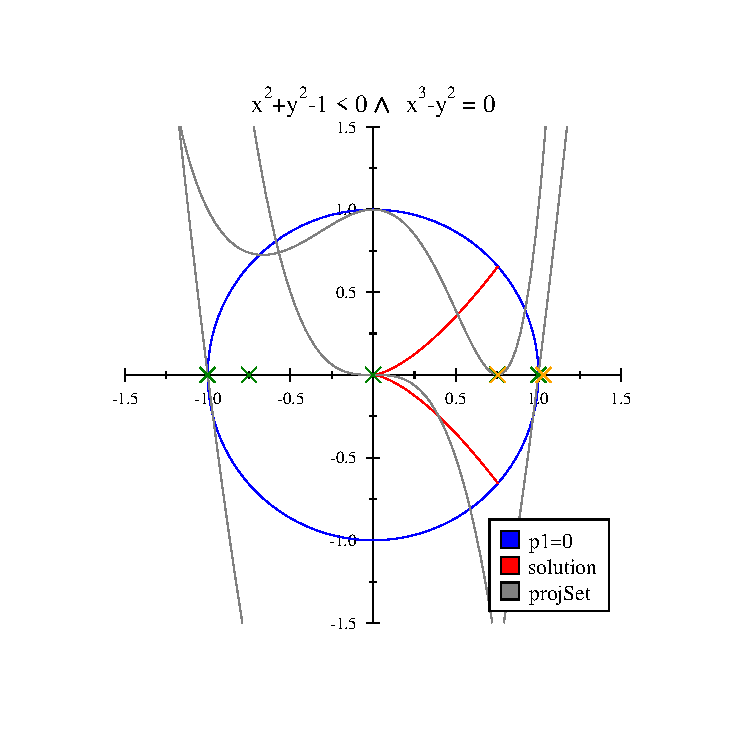
\includegraphics[scale=1.0]{cad1.eps}
%\caption{Example 1.}
%\label{fig:cad1}
%\end{figure}
% 
\begin{thebibliography}{1}
%
\bibitem{PMA} Walter Rudin,
  {\em Principles of Mathematical Analysis},
  International series in pure and applied mathematics,
  1976, McGraw-Hill.
\bibitem{GIT} Hassler Whitney. {\em Geometric Integration Theory},
  Princeton Mathematical Series, No. 21. Literary Licensing, LLC.
\bibitem{GMT} Herbert Federer. {\em Geometric Measure Theory}. Springer,        
  Reprint of the 1st ed. Berlin, Heidelberg, New York 1969 edition.
\bibitem{JH} Jenny Harrison, {\em Operator Calculus of Differential
  Chains and Differential Forms}, to appear in the Journal of Geometric
  Analysis, 2013. \\
  Url:\ {\small {\tt math.berkeley.edu/\textasciitilde harrison}}
\end{thebibliography}
%
\end{document}
% -----------------------------------------------------------------------------
% END DOCUMENTATION
% -----------------------------------------------------------------------------